\begin{apendicesenv}

\partapendices

\chapter{Aspectos de Gerenciamento do Projeto}
\section{Termo de abertura do Projeto}
Com uma rotina cada vez mais corrida, as pessoas têm a necessidade de agilizar ao máximo tarefas secundárias ao trabalho/estudo e, em seu máximo, automatizá-las. Com o objetivo de ser um facilitador na manutenção e limpeza de pisos, o Quirby surge como uma alternativa para manter sempre o chão de uma casa limpa, sem tomar muito tempo do morador, não atrapalhando, assim, sua rotina.
\subsection{Objetivo do Projeto}
O projeto visa desenvolver um robô aspirador que esteja ao nível dos já existentes no mercado porém com conectividade, sendo isso um diferencial em relação aos modelos de mesma faixa de preço.
\subsection{Equipe Responsável}
\subsubsection{Subequipe de Eletrônica}

Alander Praxedes de Souza Oliveira,
Gustavo Raspante Faria,
Fernando Souza Braga,
Murilo de Souza Barcelos,
Estéfane Mendes do Nascimento.
\subsubsection{Subequipe de Software}
Marcos Vinícius Rodrigues da Conceição,
Bruno Carmo Nunes,
João Paulo Coelho de Souza,
Estevão de Jesus Reis,
Hérya Rodrigues Alcantara,
Giovana Vitor Dionisio Santana,
Gabriel Azevedo Batalha.

\subsubsection{Subequipe de Estrutura}
Matheus Rodrigues de C. Silva,
Igo de França Lino.
\subsection{Estruturação do Projeto}
A equipe de trabalho foi dividida em três: Software, eletrônica e estruturas. A de software ficando responsável pelo desenvolvimento do algoritmo do robô e do aplicativo para controle do mesmo; eletrônica por toda a parte elétrica e eletrônica do Quirby; e estruturas pelo desenvolvimento e confecção da carcaça e possíveis acessórios do mesmo.
\subsubsection{EAP Estrutura Analítica do Projeto}
A Estrutura Analítica do Projeto (EAP) apresenta a subdivisão das entregas, das atividades e do trabalho do projeto em componentes menores, de forma a facilitar o gerenciamento e entendimento do projeto. O tópico \ref{EAP} apresenta a  EAP geral do projeto Quirby, englobando o Gerenciamento e os subsistemas de Estrutura, Eletrônica e Software, e as EAPs de cada subsistema.
\subsubsection{Marcos e Entregas principais}
Os marcos do projeto, ou as fases, assim como as atividades que os compõem podem ser vistos no tópico “Definição de atividades e cronograma de execução”, ainda neste capítulo, na Tabela \ref{tab cronograma}. As entregas principais são PC1 (fases 1 e 2), PC2 (fase 3) e PC3 (fase 4). 
\subsection{Principais Requisitos}
Os principais requisitos do projeto, funcionais e não funcionais, foram listados no item \ref{requisitos} do presente relatório.
\subsection{Riscos do Projeto}
Os riscos do projeto, assim como suas consequências e planos de contingência estão listados no item \ref{levantamento de riscos} do relatório.
\subsection{Recursos e Orçamento do Projeto}
Para a realização do presente projeto, os recursos serão advindos de um fundo criado pelo grupo de trabalho e abastecido pelos próprios membros da equipe. Em um primeiro momento, o projeto está orçado em R\$\ 1061,30. O detalhamento do orçamento está presente no item \ref{orçamento} do presente relatório.
\section{Lista É/Não É}
A Tabela \ref{tab} apresenta as noções e concepções básicas acerca do que o produto é e não é, para facilitar o levantamento e entendimento de seus objetivos e escopo \cite{caroli}.

\begin{table}[H]
\centering
\caption{\label{Tab 5} Lista É / Não É}
\begin{tabular}{
>{\columncolor[HTML]{DBEEF3}}l 
>{\columncolor[HTML]{DBEEF3}}l lll}
\multicolumn{1}{c}{\cellcolor[HTML]{D9D9D9}\textbf{É}} & \multicolumn{1}{c}{\cellcolor[HTML]{D9D9D9}\textbf{NÃO É}} &  &  &  \\
Robô aspirador semi autônomo                           & Para limpeza industrial                                    &  &  &  \\
Robô de limpeza                                        & 100\% autônomo                                             &  &  &  \\
Robô inteligente que aspira pó                         & Projetado para ambientes abertos                           &  &  &  \\
                       &                                                            &  &  &  \\
Facilitador da limpeza do Lar                          &                                                            &  &  & 
\end{tabular}
\label{tab}
\end{table}
 




\end{apendicesenv}
\section{Organização da Equipe}
Nessa seção, será mostrada como a equipe está organizada para a realização do projeto.

\subsection{Organograma}

\begin{figure}[h!]
\centering
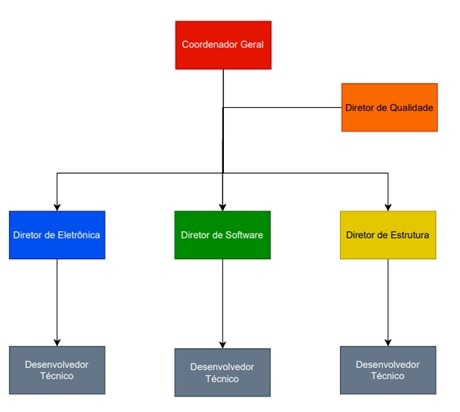
\includegraphics[width= 11.25cm, height=11.25cm]{figuras/Fig9.jpg}
\caption{Organograma \\ Fonte: Autoria própria, 2023}
\label{Fig9}
\end{figure}

\subsection{Plano de comunicação}
A comunicação do grupo será realizada por meio de reuniões presenciais e utilização de ferramentas de comunicação.
Serão realizadas reuniões presenciais entre os membros da equipe de projeto duas vezes por semana, no horário das aulas.
Durante a execução do projeto, serão utilizadas ferramentas de comunicação e gerenciamento de projeto para o acompanhamento e monitoramento das atividades e trabalhos. As ferramentas utilizadas serão:
\begin{itemize}
 \item Discord: Ferramenta utilizada para a realização de reuniões de forma remota; 
\item Microsoft Planner:  Ferramenta utilizada para distribuição, organização e acompanhamento do progresso de tarefas; 
\item Google Drive: Ferramenta utilizada para compartilhamento e edição simultânea de arquivos e documentos; 
\item Telegram: Ferramenta utilizada para comunicação rápida através de troca de mensagens;
\item Github: Ferramenta utilizada para controle de versão dos artefatos de software.

\end{itemize}
\section{Repositórios}
\begin{itemize}
\item Link da organização no Github, onde são armazenados os artefatos de software: \url{https://github.com/PI2-Grupo5}
\item Link do Google Drive, onde estão armazenados os arquivos e documentos compartilhados da equipe: \url{https://drive.google.com/drive/folders/1tdZdirz2VFmGbvBSTcqoBoK9ebg5-t-A}
\item Link para o Mural, onde encontram-se as informações referentes às etapas realizadas durante o Lean Inception: \url{https://app.mural.co/t/pi29130/m/pi29130/1668640826591/79657b24d3121358f8728955e03758c67b16af15?invited=true&sender=u64465818e1a890ee67403043} 
\end{itemize}
\section{EAP (Estrutura Analítica de Projeto) Geral do Projeto}
\label{EAP}
A Estrutura Analítica do Projeto (EAP) apresenta a subdivisão das entregas, das atividades e do trabalho do projeto em componentes menores, para facilitar o gerenciamento e entendimento do projeto. A Figura \ref{Fig10-Eap} apresenta a EAP geral do projeto Quirby, englobando o Gerenciamento e os subsistemas de Estrutura, Eletrônica e Software.

\begin{figure}[H]
\begin{center}
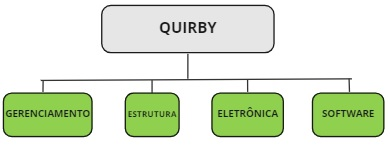
\includegraphics[width= 11.5 cm, height = 5cm]{figuras/Fig10.jpg}
\caption{EAP geral do projeto \\ Fonte: Autoria própria, 2023}
\label{Fig10-Eap}
\end{center}
\end{figure}

\subsection{Papeis e Responsabilidades}
Os diretores de cada área do projeto ficarão responsáveis pela avaliação de qualidade e melhoria contínua dos subsistemas do processo de integração e também pelo funcionamento e testes destes.
\subsection{EAP do Subsistema de Estrutura}
A figura abaixo apresenta a EAP do subsistema de Estrutura.
\begin{figure}[H]
\begin{center}
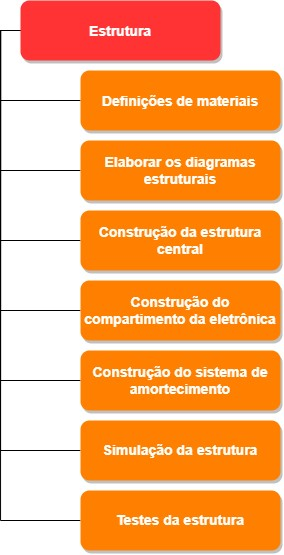
\includegraphics[width= 5cm, height=8cm]{figuras/Fig11.jpg}
\caption{EAP do subsistema de Estrutura \\ Fonte: Autoria própria, 2023}
\label{Fig11}
\end{center}
\end{figure}

\subsection{EAP do Subsistema de Eletrônica}
A figura abaixo apresenta a EAP do subsistema de Eletrônica.

%consetar posição da imagem
\begin{figure}[H]
\begin{center}
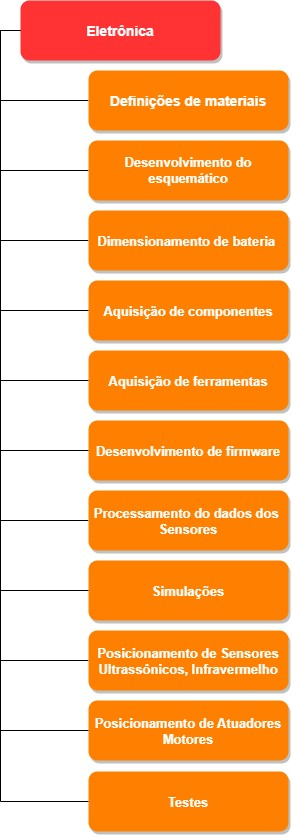
\includegraphics[width= 5cm, height=11cm]{figuras/Fig12.jpg}
\caption{EAP do subsistema de Eletrônica \\ Fonte: Autoria própria, 2023}
\label{Fig12}
\end{center}
\end{figure}

\subsection{EAP do Subsistema de Software}
A figura abaixo apresenta a EAP do subsistema de Software.

%consetar posição da imagem
\begin{figure}[H]
\begin{center}
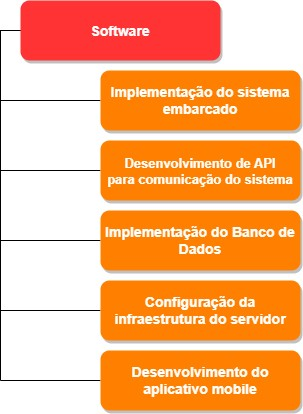
\includegraphics[width= 6cm, height=8cm]{figuras/Fig13.jpg}
\caption{EAP do subsistema de Software \\ Fonte: Autoria prórpia, 2023}
\label{Fig13}
\end{center}
\end{figure}

\section{Definição de atividades e Cronograma de Execução}
Segundo JUSTO (2019), o Gerenciamento de Cronograma é a união dos processos necessários para assegurar a execução do projeto em tempo hábil. Ele mostra uma visão geral das atividades e das relações entre elas, além de mostrar os prazos das atividades e o prazo final do projeto.
Na Tabela \ref{tab 6} é possível visualizar as datas estipuladas para início e fim do projeto, enquanto na Tabela \ref{tab cronograma} é apresentado o cronograma geral das atividades do projeto Quirby:

\begin{table}[H]
\centering
\caption{\label{tab 6} Início e Fim de projeto}
\begin{tabular}{
>{\columncolor[HTML]{DBEEF3}}c 
>{\columncolor[HTML]{DBEEF3}}c l}
\cellcolor[HTML]{D9D9D9}\textbf{Geral} & \cellcolor[HTML]{D9D9D9}\textbf{Data} &  \\
Início do Projeto                      & 07/11/2022                            &  \\
Fim do Projeto                         & 02/02/2023                            & 
\end{tabular}
\end{table}

\\

\begin{table}[H]
\caption{\label{tab cronograma} Cronograma de Atividades}
\begin{tabular}{|c|c|c|c|c|}
\hline
\rowcolor[HTML]{D9D9D9} 
\textbf{Nº}            & \textbf{Atividade}                                                                                                     & \textbf{Início}       & \textbf{Fim}          & \textbf{Responsável}                                                                                             \\ \hline
\rowcolor[HTML]{DBEEF3} 
1                      & \textbf{Fase 1: Problematização}                                                                                       & 07/11/22              & 24/11/22              & -                                                                                                                \\ \hline
\rowcolor[HTML]{DBEEF3} 
1.1                    & \begin{tabular}[c]{@{}c@{}}Identificar escopo \\ do projeto\end{tabular}                                               & 07/11/22              & 14/11/22              & Todos                                                                                                            \\ \hline
\rowcolor[HTML]{DBEEF3} 
1.1.1                  & Definir escopo                                                                                                         & 207/11/22             & 14/11/22              & Todos                                                                                                            \\ \hline
\rowcolor[HTML]{DBEEF3} 
1.1.2                  & \begin{tabular}[c]{@{}c@{}}Analisar viabilidade \\ técnica e financeira\end{tabular}                                   & 07/11/22              & 14/11/22              & Todos                                                                                                            \\ \hline
\rowcolor[HTML]{DBEEF3} 
1.1.3                  & \begin{tabular}[c]{@{}c@{}}Refinar Requisitos \\ funcionais e não \\ funcionais\end{tabular}                           & 07/11/22              & 14/11/22              & Todos                                                                                                            \\ \hline
\rowcolor[HTML]{DBEEF3} 
1.1.4                  & \begin{tabular}[c]{@{}c@{}}Refinar entendimento \\ do problema\end{tabular}                                            & 07/11/22              & 14/11/22              & Todos                                                                                                            \\ \hline
\rowcolor[HTML]{DBEEF3} 
1.2                    & \begin{tabular}[c]{@{}c@{}}Documentar escopo\\ definido referente \\ a fase 1\end{tabular}                             & 07/11/22              & 14/11/22              & Todos                                                                                                            \\ \hline
\rowcolor[HTML]{DBEEF3} 
2                      & \textbf{\begin{tabular}[c]{@{}c@{}}Fase 2: Concepção e \\ detalhamento da solução\end{tabular}}                        & 15/11/22              & 21/11/22              & Todos                                                                                                            \\ \hline
\rowcolor[HTML]{DBEEF3} 
2.1                    & \begin{tabular}[c]{@{}c@{}}Definir o Termo de \\ Abertura do Projeto\end{tabular}                                      & 15/11/22              & 21/11/22              & Todos                                                                                                            \\ \hline
\rowcolor[HTML]{DBEEF3} 
2.2                    & Criar Estrutura da EAP                                                                                                 & 15/11/22              & 21/11/22              & Todos                                                                                                            \\ \hline
\rowcolor[HTML]{DBEEF3} 
2.2                    & Descrever os requisitos                                                                                                & 15/11/22              & 24/11/22              & Todos                                                                                                            \\ \hline
\rowcolor[HTML]{DBEEF3} 
2.3                    & \begin{tabular}[c]{@{}c@{}}Definir cronograma de\\  Atividades\end{tabular}                                            & 15/11/22              & 24/11/22              & Todos                                                                                                            \\ \hline
\rowcolor[HTML]{DBEEF3} 
2.4                    & \begin{tabular}[c]{@{}c@{}}Estimar custos do \\ projeto\end{tabular}                                                   & 15/11/22              & 24/11/22              & Todos                                                                                                            \\ \hline
\rowcolor[HTML]{DBEEF3} 
2.5                    & \begin{tabular}[c]{@{}c@{}}Definir recursos \\ humanos do projeto\end{tabular}                                         & 15/11/22              & 24/11/22              & Todos                                                                                                            \\ \hline
\rowcolor[HTML]{DBEEF3} 
2.6                    & \begin{tabular}[c]{@{}c@{}}Identificar riscos \\ do projeto\end{tabular}                                               & 15/11/22              & 24/11/22              & Todos                                                                                                            \\ \hline
\rowcolor[HTML]{DBEEF3} 
2.4                    & \begin{tabular}[c]{@{}c@{}}Elaborar plano de \\ contingência para \\ os riscos\end{tabular}                            & 15/11/22              & 24/11/22              & Todos                                                                                                            \\ \hline
\rowcolor[HTML]{DBEEF3} 
2.4                    & \begin{tabular}[c]{@{}c@{}}Descrever arquitetura \\ de cada subsistema\end{tabular}                                    & 15/11/22              & 24/11/22              & Todos                                                                                                            \\ \hline
\rowcolor[HTML]{DBEEF3} 
3                      & \textbf{\begin{tabular}[c]{@{}c@{}}Fase 3: Projeto e construção \\ de subsistemas da \\ solução proposta\end{tabular}} & 25/11/22              & 02/01/23              & Todos                                                                                                            \\ \hline
\rowcolor[HTML]{DBEEF3} 
3.1                    & \begin{tabular}[c]{@{}c@{}}Fabricar a carcaça \\ do Quirby\end{tabular}                                                & 25/11/22              & 02/01/23              & \begin{tabular}[c]{@{}c@{}}Matheus Rodrigues, \\ Igo de França\end{tabular}                                      \\ \hline
\rowcolor[HTML]{DBEEF3} 
3.2                    & \begin{tabular}[c]{@{}c@{}}Fazer a montagem dos \\ sistemas eletrônicos\end{tabular}                                   & 25/11/22              & 02/01/23              & \begin{tabular}[c]{@{}c@{}}Alander Praxedes, \\ Fernando Braga, \\ Gustavo Raspante\end{tabular}                 \\ \hline
\rowcolor[HTML]{DBEEF3} 
3.4                    & \begin{tabular}[c]{@{}c@{}}Desenvolver o sistema \\ de consumo energético \\ e recarga do Quirby\end{tabular}           & 25/11/22              & 02/01/23              & \begin{tabular}[c]{@{}c@{}}Estéfane Mendes, \\ Murilo Barcelos\end{tabular}                                      \\ \hline
\rowcolor[HTML]{DBEEF3} 
3.5                    & \begin{tabular}[c]{@{}c@{}}Desenvolver o \\ back-end\end{tabular}                                                      & 25/11/22              & 20/12/23              & \begin{tabular}[c]{@{}c@{}}Gabriel Batalha, \\ Bruno Nunes, \\ João Souza\end{tabular}                           \\ \hline
\rowcolor[HTML]{DBEEF3} 
\end{tabular}
\end{table}

\begin{table}[H]
\begin{tabular}{|c|c|c|c|c|}
\hline
\rowcolor[HTML]{DBEEF3}
3.6                    & \begin{tabular}[c]{@{}c@{}}Desenvolver o \\ aplicativo mobile\end{tabular}                                             & 25/11/22              & 20/12/23              & \begin{tabular}[c]{@{}c@{}}Marcos Vinícius,\\  Estevão Reis, \\ Hérya Rodrigues, \\ Giovana Santana\end{tabular} \\ \hline
\rowcolor[HTML]{DBEEF3} 
3.7                    & \begin{tabular}[c]{@{}c@{}}Fazer a Integração \\ do back-end com \\ o mobile\end{tabular}                              & 20/12/23              & 02/12/23              & \begin{tabular}[c]{@{}c@{}}Subsistema de \\ Software\end{tabular}                                                \\ \hline
\rowcolor[HTML]{DBEEF3} 
3.8                    & \begin{tabular}[c]{@{}c@{}}Desenvolver o relatório\\  para o ponto de \\ controle 2\end{tabular}                       & 25/11/22              & 02/01/23              & Todos                                                                                                            \\ \hline
\rowcolor[HTML]{DBEEF3} 
4                      & \textbf{\begin{tabular}[c]{@{}c@{}}Fase 4: Integração de\\  subsistemas e finalização \\ do produto\end{tabular}}      & 03/01/23              & 27/01/2023            & Todos                                                                                                            \\ \hline
\rowcolor[HTML]{DBEEF3} 
4.1                    & \begin{tabular}[c]{@{}c@{}}Integrar componentes \\ da solução\end{tabular}                                             & 03/01/23              & 13/01/23              & Todos                                                                                                            \\ \hline
\rowcolor[HTML]{DBEEF3} 
4.2                    & \begin{tabular}[c]{@{}c@{}}Testar o produto final \\ e comprovar o funcionamento\\  da solução\end{tabular}            & 16/01/23              & 20/01/23              & Todos                                                                                                            \\ \hline
\rowcolor[HTML]{DBEEF3} 
4.3                    & \begin{tabular}[c]{@{}c@{}}Avaliar e homologar \\ o produto final do \\ projeto\end{tabular}                           & 23/01/23              & 27/01/23              & Todos                                                                                                            \\ \hline
\rowcolor[HTML]{DBEEF3} 
4.4                    & \begin{tabular}[c]{@{}c@{}}Desenvolver o relatório\\  para o ponto de controle 3\end{tabular}                          & 03/01/23              & 27/01/2023            & Todos                                                                                                                                                 \\ \hline
\end{tabular}
\end{table}
\section{Levantamento de Riscos}
\label{levantamento de riscos}
Amplamente divulgado através do PMBOK, o Gerenciamento de Riscos propõe a identificação de riscos e planos de ação para mitigá-los, eliminá-los, ou mesmo transferi-los \cite{pmi} . Dentre eles, destacam-se os riscos apresentados nas Tabelas \ref{tab 8}, \ref{tab 9}, \ref{tab externos} e \ref{tab 10}.

\begin{itemize}
   \item \textbf{Riscos de Projeto}
\end{itemize}

\begin{table}[H]
\caption{\label{tab 8} Registro de Riscos}
\begin{tabular}{ |>{\centering\arraybackslash} m{0.5cm}|>{\centering\arraybackslash} m{3.5cm} |>{\centering\arraybackslash} m{5.5cm} |>{\centering\arraybackslash} m{5.5cm} |}
\hline
\rowcolor[HTML]{D9D9D9} 
\textbf{Nº} & \textbf{Riscos}                                                                     & \multicolumn{1}{c|}{\cellcolor[HTML]{D9D9D9}\textbf{Consequência}}                                                                           & \textbf{Contingência}                                                                                                                      \\ \hline
\rowcolor[HTML]{DBEEF3} 
1           & \begin{tabular}[c]{@{}c@{}}Indefinição do \\ escopo\end{tabular}                    & \begin{tabular}[c]{@{}l@{}}Alteração no planejamento \\ e andamento das sprints\end{tabular}                                                 & Definir o escopo                                                                                                                           \\ \hline
\rowcolor[HTML]{DBEEF3} 
2           & \begin{tabular}[c]{@{}c@{}}Mudança do \\ escopo\end{tabular}                        & \begin{tabular}[c]{@{}l@{}}Alteração no planejamento \\ e andamento das sprints\end{tabular}                                                 & \begin{tabular}[c]{@{}c@{}}Organizar novamente\\  as sprints\end{tabular}                                                                  \\ \hline
\rowcolor[HTML]{DBEEF3} 
3           & \begin{tabular}[c]{@{}c@{}}Imaturidade da \\ gerência\end{tabular}                  & \begin{tabular}[c]{@{}l@{}}Planejamentos falhos, \\ falta de qualidade, aumento\\  do custo e tempo do projeto,\\  entre outros\end{tabular} & Trocar a gerência                                                                                                                          \\ \hline
\rowcolor[HTML]{DBEEF3} 
4           & \begin{tabular}[c]{@{}c@{}}Alteração na \\ arquitetura\end{tabular}                 & \begin{tabular}[c]{@{}l@{}}Gera retrabalho, alteração\\ nas histórias planejadas, \\ mudança de infraestrutura\\  e código\end{tabular}      & \begin{tabular}[c]{@{}c@{}}Analisar se é a melhor \\ alternativa mudar\\  arquitetura\end{tabular}                                         \\ \hline
\rowcolor[HTML]{DBEEF3} 
5           & \begin{tabular}[c]{@{}c@{}}Comunicação não \\ eficiente do grupo\end{tabular}       & \begin{tabular}[c]{@{}l@{}}Falhas de desenvolvimento,\\ perda de informação \\ e retrabalho\end{tabular}                                        & \begin{tabular}[c]{@{}c@{}}Estruturar um padrão \\ de comunicação no time\end{tabular}                                                     \\ \hline
\rowcolor[HTML]{DBEEF3} 
6           & \begin{tabular}[c]{@{}c@{}}Baixa produtividade \\ dos integrantes\end{tabular}      & \begin{tabular}[c]{@{}l@{}}Risco para o planejamento e \\ aumento de tarefas \\não concluídas\end{tabular}                                     & \begin{tabular}[c]{@{}c@{}}Reorganização das tarefas \\ e em último caso, \\ retirada de membros \\ que atrapalham o time\end{tabular}     \\ \hline
\rowcolor[HTML]{DBEEF3} 
7           & \begin{tabular}[c]{@{}c@{}}Divergência de\\ horários\\ entres os membros\end{tabular} & \begin{tabular}[c]{@{}l@{}}Risco para o planejamento \\ e aumento de tarefas não \\ concluídas\end{tabular}                                  & \begin{tabular}[c]{@{}c@{}}Tentar alocar aqueles com \\ horários compatíveis e os \\ que não tem trabalham\\  individualmente\end{tabular} \\ \hline
\rowcolor[HTML]{DBEEF3} 
8           & \begin{tabular}[c]{@{}c@{}}Dificuldades na \\ integração do time\end{tabular}       & \begin{tabular}[c]{@{}l@{}}Risco para o planejamento\\ e aumento de tarefas não \\ concluídas\end{tabular}                                   & \begin{tabular}[c]{@{}c@{}}Procurar divergências para \\ solucionar e novas técnico \\ de entrosamento\end{tabular}                        \\ \hline
\rowcolor[HTML]{DBEEF3} 
9           & \begin{tabular}[c]{@{}c@{}}Saída de membro \\ do grupo\end{tabular}                 & \begin{tabular}[c]{@{}l@{}}Sobrecarga e desgaste \\ dos demais membros \\ do grupo\end{tabular}                                              & \begin{tabular}[c]{@{}c@{}}Redistribuição de tarefas \\ de acordo com afinidade\\  de conteúdo\end{tabular}                                \\ \hline
\rowcolor[HTML]{DBEEF3} 
10          & \begin{tabular}[c]{@{}c@{}}Falta de dedicação \\ em atividades\end{tabular}         & \begin{tabular}[c]{@{}l@{}}Risco para o planejamento\\  e aumento de tarefas\\  não concluídas\end{tabular}                                  & \begin{tabular}[c]{@{}c@{}}Reuniões para motivar \\ o time\end{tabular}                                                                    \\ \hline
\rowcolor[HTML]{DBEEF3} 
11          & Atividades atrasadas                                                                & \begin{tabular}[c]{@{}l@{}}Risco para o planejamento \\ e aumento de tarefas \\ não concluídas\end{tabular}                                  & \begin{tabular}[c]{@{}c@{}}Procurar o motivo dos \\ atrasos e solucionar\end{tabular}                                                      \\ \hline
\rowcolor[HTML]{DBEEF3} 
12          & \begin{tabular}[c]{@{}c@{}}Atividades \\ secundárias  dos\\ membros\end{tabular}       & \begin{tabular}[c]{@{}l@{}}Risco para o planejamento\\  e aumento de tarefas\\  não concluídas\end{tabular}                                  & \begin{tabular}[c]{@{}c@{}}Encaixar os horários\\ disponíveis  dos membros \\na agenda do time\end{tabular}                                  \\ \hline
\end{tabular}
\end{table}

\begin{itemize}
    \item \textbf{Riscos Técnicos}
\end{itemize}

\begin{table}[H]
\caption{\label{tab 9} Riscos Técnicos}
\begin{tabular}{|c|c|c|c|}
\hline
\rowcolor[HTML]{D9D9D9} 
\textbf{Nº} & \textbf{Riscos}                                                           & \textbf{Consequência}                                                                    & \textbf{Contingência}                                                                                                                   \\ \hline
\rowcolor[HTML]{DBEEF3} 
1           & \begin{tabular}[c]{@{}c@{}}Falta ou falha \\ de equipamentos\end{tabular} & \begin{tabular}[c]{@{}c@{}}Prejudica o planejamento\\  e atrasa as entregas\end{tabular} & \begin{tabular}[c]{@{}c@{}}Buscar novos equipamentos \\ assim que constatado o problema\end{tabular}                                    \\ \hline
\rowcolor[HTML]{DBEEF3} 
2           & \begin{tabular}[c]{@{}c@{}}Dificuldade com\\ versionamento\end{tabular}   & \begin{tabular}[c]{@{}c@{}}Inviabiliza o desenvolvimento\\  do projeto\end{tabular}      & \begin{tabular}[c]{@{}c@{}}Treinamento de git ou outras \\ ferramentas de versionamento \\ para os membros com dificuldade\end{tabular} \\ \hline
\rowcolor[HTML]{DBEEF3} 
3           & \begin{tabular}[c]{@{}c@{}}Adaptação da equipe\\  com as tecnologias\end{tabular} & \begin{tabular}[c]{@{}c@{}}Prejudica o planejamento\\  e atrasa as entregas\end{tabular} & \begin{tabular}[c]{@{}c@{}}Treinar toda a equipe \\ no uso das ferramentas\end{tabular}                                                 \\ \hline
\end{tabular}
\end{table}

\begin{itemize}
    \item \textbf{Riscos Externos}
\end{itemize}

\begin{table}[H]
\caption{\label{tab externos} Riscos Externos}
\begin{tabular}{cccc}
\rowcolor[HTML]{D9D9D9} 
\textbf{Nº} & \textbf{Riscos}       & \textbf{Consequência}                                                               & \textbf{Contingência}                                                                                          \\
\rowcolor[HTML]{DBEEF3} 
1           & Questões burocráticas & \begin{tabular}[c]{@{}c@{}}Pode inviabilizar o \\ andamento do projeto\end{tabular} & \begin{tabular}[c]{@{}c@{}}Resolver as questões \\ burocráticas antes de dar\\  início ao projeto\end{tabular}
\end{tabular}
\end{table}

\begin{itemize}
    \item \textbf{Riscos do Produto}
\end{itemize}

\begin{table}[H]
\caption{\label{tab 10} Riscos do Produto}
\begin{tabular}{|c|c|c|c|}
\hline
\rowcolor[HTML]{D9D9D9} 
\textbf{Nº} & \textbf{Riscos}                                                                          & \textbf{Consequência}                                                                                                                  & \textbf{Contingência}                                                                                          \\ \hline
\rowcolor[HTML]{DBEEF3} 
1           & \begin{tabular}[c]{@{}c@{}}Produto não atende \\ às necessidades do cliente\end{tabular} & \begin{tabular}[c]{@{}c@{}}Projeto falho e\\  inutilizável\end{tabular}                                                                & \begin{tabular}[c]{@{}c@{}}Refatorar requisitos\\  e reescrever escopo\end{tabular}                            \\ \hline
\rowcolor[HTML]{DBEEF3} 
2           & \begin{tabular}[c]{@{}c@{}}Complexidade de\\  implementação\end{tabular}                 & \begin{tabular}[c]{@{}c@{}}Dificuldade na prestação\\ de manutenção e \\ correção de defeitos\end{tabular}                             & \begin{tabular}[c]{@{}c@{}}Refatorar o código para \\ verificar se a complexidade \\ está correta\end{tabular} \\ \hline
\rowcolor[HTML]{DBEEF3} 
3           & \begin{tabular}[c]{@{}c@{}}Falta de especificação\\  dos testes\end{tabular}             & \begin{tabular}[c]{@{}c@{}}Testes realizados em cada \\ departamento acabam\\  diminuindo a confiabilidade \\ do produto.\end{tabular} & \begin{tabular}[c]{@{}c@{}}Ser rígido na definição\\ e padronização dos testes\end{tabular}                    \\ \hline
\end{tabular}
\end{table}
\subsection{Visualização dos Riscos}
\begin{itemize}
    \item \textbf{Classificação dos Riscos}
\end{itemize}
O grau dos riscos é definido pela multiplicação da probabilidade de ocorrência, pelo impacto dos mesmos causados ao projeto (DEVMEDIA, 2018).
A definição das classificações de risco estão dispostas abaixo na Figura \ref{Tabela 12}.

\begin{figure}[H]
\begin{center}
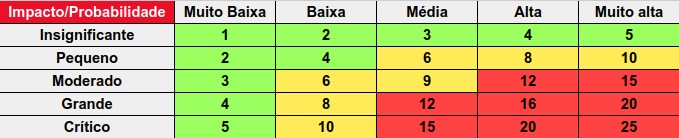
\includegraphics[width= 16cm, height=3.5cm]{figuras/Classific_risco.jpg}
\caption{Classificação de Riscos}
\label{Tabela 12}
\end{center}
\end{figure}

\begin{itemize}
    \item \textbf{Quadro de Riscos}
\end{itemize}
Seguindo um dos pilares do Scrum que diz respeito à transparência, e do PMBOK a respeito do monitoramento e gerenciamento de riscos, os riscos serão mapeados rigorosamente (e pontuados) e podem ser vistos na Figura \ref{burndownRiscos}.

\begin{figure}[h!]
\centering
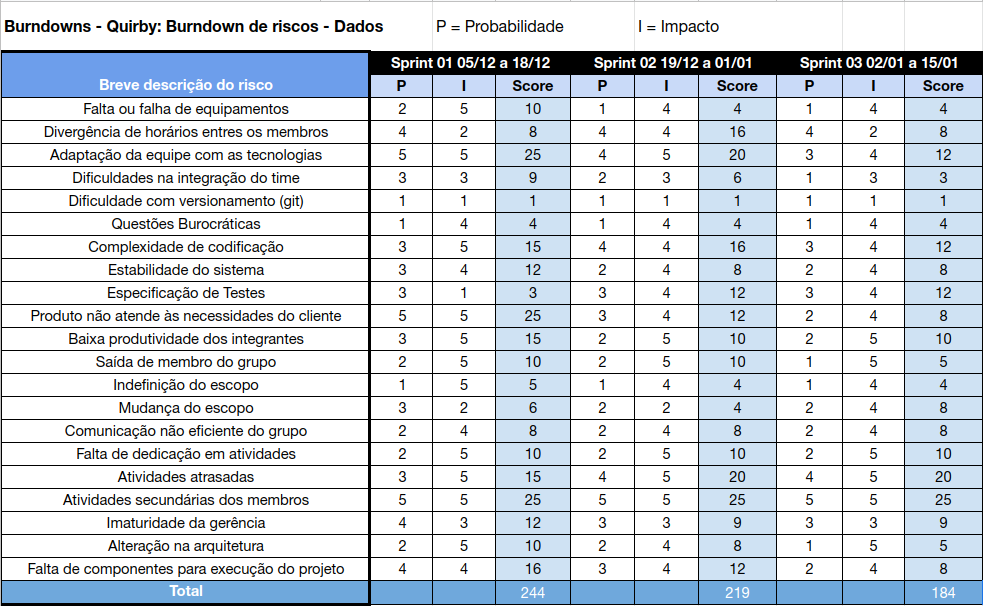
\includegraphics[width=\textwidth]{figuras/burndownRiscos.png}
\caption{Burndown de riscos}
\label{burndownRiscos}
\end{figure}

Com o passar dos sprints serão construídos gráficos onde é possível acompanhar o andamento e a progressão dos riscos associados ao desenvolvimento do projeto. Com esses dados em mãos, pode-se agir de maneira mais eficaz no controle e mitigação dos riscos.
\section{Orçamento Estimativo}
\label{orçamento}
\textbf{Introdução}

Para entender o custo inicial, é necessário agregar vários fatores que incluem um orçamento geral do negócio, pois uma gestão de custos eficiente cria condições favoráveis para que a empresa/organização possa definir novos orçamentos, investimentos, estratégias internas e metas - de curto, médio e longo prazo - por meio de uma análise detalhada da situação financeira atual.

\textbf {Objetivos}

Deve-se avaliar o custo dos componentes necessários para a criação do protótipo. Com esses valores, há então uma noção do custo em relação ao planejamento e desenvolvimento do projeto.

\textbf{Custo dos Componentes}
A tabela de custos referente a cada componente, e a quantidade, utilizada no Quirby encontra-se abaixo.
\begin{table}[H]
\caption{\label{tab 13} Custo dos Componentes}

\begin{tabular}{ |>{\centering\arraybackslash} m{2.5cm}|>{\centering\arraybackslash} m{4cm} |>{\centering\arraybackslash} m{3cm} |>{\centering\arraybackslash} m{2.3cm} | >{\centering\arraybackslash} m{2.4cm} |}


\hline
\rowcolor[HTML]{D9D9D9} 
\textbf{Componente}                            & \textbf{Descrição}                                                                                 & \textbf{Valor unitário}                       & \textbf{Quantidade}                    & \textbf{Valor Total}                         \\ \hline
\rowcolor[HTML]{DBEEF3} 
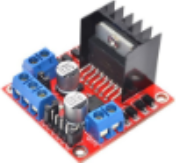
\includegraphics[scale=0.4]{figuras/ponteH.png}                                             & \begin{tabular}[c]{@{}c@{}}Driver Motor Ponte \\ H L298N\end{tabular}                              & R\$ 14,99                                     & 2                                      & R\$ 29,98                                    \\ \hline
\rowcolor[HTML]{DBEEF3} 
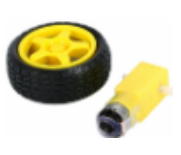
\includegraphics[scale=0.4]{figuras/conjuntoRodas.png}                                         & \begin{tabular}[c]{@{}c@{}}Motor DC 6V \\ com caixa\\ de redução e Roda\end{tabular}                  & R\$ 11,99                                     & 2                                      & R\$ 23,98                                    \\ \hline
\rowcolor[HTML]{DBEEF3} 
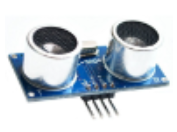
\includegraphics[scale=0.4]{figuras/sensorUltrassonico.png}                                           & \begin{tabular}[c]{@{}c@{}}Sensor Ultrassônico\\ Hc-sr04\end{tabular}                              & R\$ 7,55                                      & 3                                      & R\$ 22,65                                    \\ \hline
\rowcolor[HTML]{DBEEF3} 
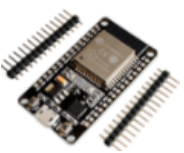
\includegraphics[scale=0.4]{figuras/esp32.png}                                         & \begin{tabular}[c]{@{}c@{}}Esp32 Wifi \\ Wroom-32\end{tabular}                                     & R\$ 38,95                                     & 1                                      & R\$ 38,95                                    \\ \hline
\rowcolor[HTML]{DBEEF3} 
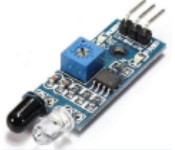
\includegraphics[scale=0.4]{figuras/sensorInfravermelho.png}                                              & \begin{tabular}[c]{@{}c@{}}Módulo Sensor de\\ Reflexão IR \\ c/ Fotodiodo\end{tabular}             & R\$ 4,25                                      & 3                                      & R\$ 12,75                                    \\ \hline
\rowcolor[HTML]{DBEEF3} 
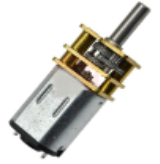
\includegraphics[scale=0.4]{figuras/motorVassouras.png}                                             & \begin{tabular}[c]{@{}c@{}}Mini Motor DC N20\\ com caixa de Redução \\ 6V 70 RPM\end{tabular}      & R\$ 28,02                                     & 2                                      & R\$ 56,04                                    \\ \hline
\rowcolor[HTML]{DBEEF3} 
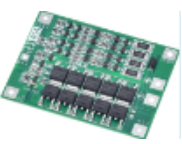
\includegraphics[scale=0.4]{figuras/bms.png}                                             & BMS 4S 40A                                                                                         & R\$ 19,00                                     & 1                                      & R\$ 19,00                                    \\ \hline
\rowcolor[HTML]{DBEEF3} 
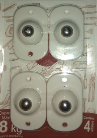
\includegraphics[scale=0.4]{figuras/rodaBoba.png}                                             & \begin{tabular}[c]{@{}c@{}}Rodízio Giratório\\\end{tabular}                     & R\$ 4,90                                      & 1                                      & R\$ 4,90                                     \\ \hline
\rowcolor[HTML]{DBEEF3} 
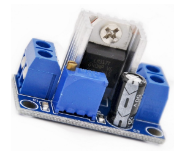
\includegraphics[scale=0.4]{figuras/StepDown.png}                                             & \begin{tabular}[c]{@{}c@{}}Conversor Dc-dc \\ Step Down Lm2596\end{tabular}                        & R\$ 7,85                                      & 2                                      & R\$ 15,70                                    \\ \hline
\rowcolor[HTML]{DBEEF3} 
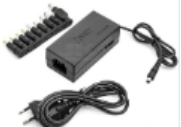
\includegraphics[scale=0.4]{figuras/fonte12V.png}                                             & \begin{tabular}[c]{@{}c@{}}Carregador Universal\\ 12V - 24V\end{tabular}                           & R\$ 30,00                                     & 1                                      & R\$ 30,00                                    \\ \hline
\rowcolor[HTML]{DBEEF3} 
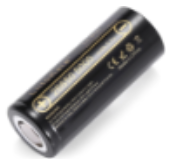
\includegraphics[scale=0.4]{figuras/bateria26650.png}                                              & \begin{tabular}[c]{@{}c@{}}Baterias 26650 \\ 3.7V 5000mAh\end{tabular}                             & R\$ 42,50                                     & 4                                      & R\$ 170,00                                   \\ \hline
\end{tabular}
\end{table}

\begin{table}[H]
\caption{\label{tab 14} Custo dos Componentes}

\begin{tabular}{ |>{\centering\arraybackslash} m{2.5cm}|>{\centering\arraybackslash} m{4cm} |>{\centering\arraybackslash} m{3cm} |>{\centering\arraybackslash} m{2.3cm} | >{\centering\arraybackslash} m{2.4cm} |}


\hline
\rowcolor[HTML]{D9D9D9} 
\textbf{Componente}                            & \textbf{Descrição}                                                                                 & \textbf{Valor unitário}                       & \textbf{Quantidade}                    & \textbf{Valor Total}                         \\ \hline
\rowcolor[HTML]{DBEEF3} 
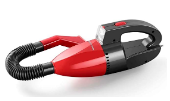
\includegraphics[scale=0.4]{figuras/aspirador.png}                                             & \begin{tabular}[c]{@{}c@{}}Conjunto Motor DC\\  12V Aspirador\end{tabular}                         & R\$ 60,00                                     & 1                                      & R\$ 60,00                                    \\ \hline
\rowcolor[HTML]{DBEEF3} 
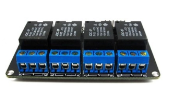
\includegraphics[scale=0.4]{figuras/reles.png}                                              & \begin{tabular}[c]{@{}c@{}}Módulo Relê\\  5v 10A\end{tabular}                                      & R\$ 13,90                                     & 2                                      & R\$ 13,90                                    \\ \hline
\rowcolor[HTML]{DBEEF3} 
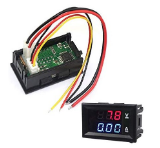
\includegraphics[scale=0.4]{figuras/voltimetroAmperimetro.png}                                               & \begin{tabular}[c]{@{}c@{}}Mini Voltímetro\\Amperímetro Digital\\ 10A\end{tabular}             & R\$ 26,90                                     & 1                                      & R\$ 26,90                                    \\ \hline
\rowcolor[HTML]{DBEEF3} 
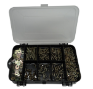
\includegraphics[scale=0.6]{figuras/maletaParafusos.png}                                              & \begin{tabular}[c]{@{}c@{}}Conjunto de parafusos, \\ porcas, arruelas \\ M3 430 peças\end{tabular} & R\$ 45,90                                     & 1                                      & R\$ 43,90                                    \\ \hline
\rowcolor[HTML]{DBEEF3} 

\includegraphics[scale=0.6]{figuras/heroku.png}                                              & 1 mês de Cloud Service                                                                             & R\$ 26,75                                     & 1                                      & R\$ 26.75                                    \\ \hline
\rowcolor[HTML]{DBEEF3} 
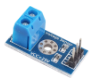
\includegraphics[scale=0.6]{figuras/sensorTensao.png}                                              & Sensor de Tensão (0-25VDC)                                                                            & R\$ 4,50                                     & 2                                      & R\$ 9,00                                    \\ \hline
\rowcolor[HTML]{DBEEF3} 
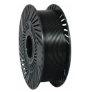
\includegraphics[scale=0.6]{figuras/plaPreto.png}                                              & 1 Kg PLA preto                                                                            & R\$ 121,01                                     & 1                                      & R\$ 121,01                                    \\ \hline
\rowcolor[HTML]{DBEEF3} 
\multicolumn{1}{|l|}{\cellcolor[HTML]{DBEEF3}} & \multicolumn{1}{l|}{\cellcolor[HTML]{DBEEF3}}                                                      & \multicolumn{1}{l|}{\cellcolor[HTML]{DBEEF3}} & \cellcolor[HTML]{00FF00}\textbf{Total} & \cellcolor[HTML]{00FF00}\textbf{R\$ 834,12} \\ \hline
\end{tabular}
\end{table}







































Para a produção do MVP estimado em 3 meses de duração, o custo do MVP é estimado em \textbf{R\$\ 834,12}. Os componentes conseguidos de maneira gratuita serão discriminados posteriormente neste relatório e o custo total atualizado.

\section{Alocação de Recursos Humanos}
O gerenciamento dos recursos humanos do projeto inclui os processos que organizam e gerenciam a equipe do projeto. A equipe do projeto consiste nas pessoas com papéis e responsabilidades designadas para a conclusão do projeto. No projeto as áreas de atuação: eletrônica, software e estrutura, devem contar com áreas de conhecimentos específicos em cada subsistema para o planejamento, desenvolvimento, gestão e execução do produto final. Na Figura \ref{Alocação de Recursos Humanos} é destacado os recursos humanos necessários para o desenvolvimento do projeto por completo.

\begin{figure}[h!]
\begin{center}
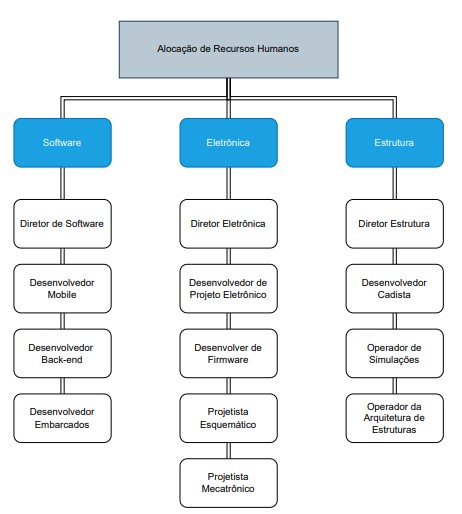
\includegraphics[width= 10cm, height=11cm]{figuras/Recursos_humanos.jpg}
\caption{Alocação de Recursos Humanos}
\label{Alocação de Recursos Humanos}
\end{center}
\end{figure}

% \chapter{Desenhos Técnicos mecânicos}
\begin{comment}
Desenhos técnicos mecânicos: indicação de cotas, cortes (se necessário), elementos de fixação, simbologia de soldagem (se necessário), lista de elementos e materiais em desenhos de conjunto, nas legendas indicação do tipo de material, unidade, massa do elemento, escala, diedro, projetista ou desenhista, revisor, dentre outras informações que auxiliem na fabricação das estruturas mecânicas do sistema. Vide item 7 do apêndice 03; 
\end{comment}

\chapter{Diagramas elétricos e eletrônicos}
\begin{comment}
Diagramas elétricos e eletrônicos do sistema: sendo compostos por diagramas unifilares/trifilares (com os dispositivos de proteção, seccionamento, seção de fios, etc.) de sistemas de alimentação, diagramas esquemáticos de circuitos eletrônicos (com identificação dos componentes eletrônicos que serão utilizados nos circuitos), diagramas detalhando barramentos de alimentação dos circuitos eletrônicos (ou seja, trata-se da interface entre sistemas de alimentação e circuitos eletrônicos), diagramas com detalhes de lógicas e protocolos de comunicação entre elementos (microcontrolador com microcontrolador, microcontrolador e sensor, microcontrolador e atuador, microcontrolador e software, etc); 
\end{comment}
% Se for necessário
% \chapter{Diagramas de sistemas térmicos e/ou hidráulicos}

\chapter{Documentação de software}
\begin{comment}
Introdução: Pequeno texto apresentará, com objetividade, o propósito da solução de software, e como vêem a integração com outras Engenharia. Também, introduzirá os seguintes tópicos.  

(a) Arquitetura da Informação->  deve-se apresentar as telas, estruturas de navegação, aspectos associados ao design da solução com a utilização de ferramentas como o Figma ou similares; 


(b) Inovação-> Deve-se apresentar um texto destacando-se as principais inovações a serem realizadas no projeto pela equipe de software. É desejável que haja uma pequena revisão bibliográfica para fundamentar aspectos associados a este tópico.  

(c) Diagramas -> Apresentação e comentários quanto aos diagramas em geral necessários para apresentar a solução proposta: diagramas de classes, diagramas de casos de uso, diagramas com protocolos de comunicação entre componentes do software, protótipos de telas, etc. 

\end{comment}

\section{Protótipo de Baixa-Média Fidelidade}
\label{prototipo}
\subsection{Tela de Cadastro e Login}
\begin{figure}[H]
\centering
\frame{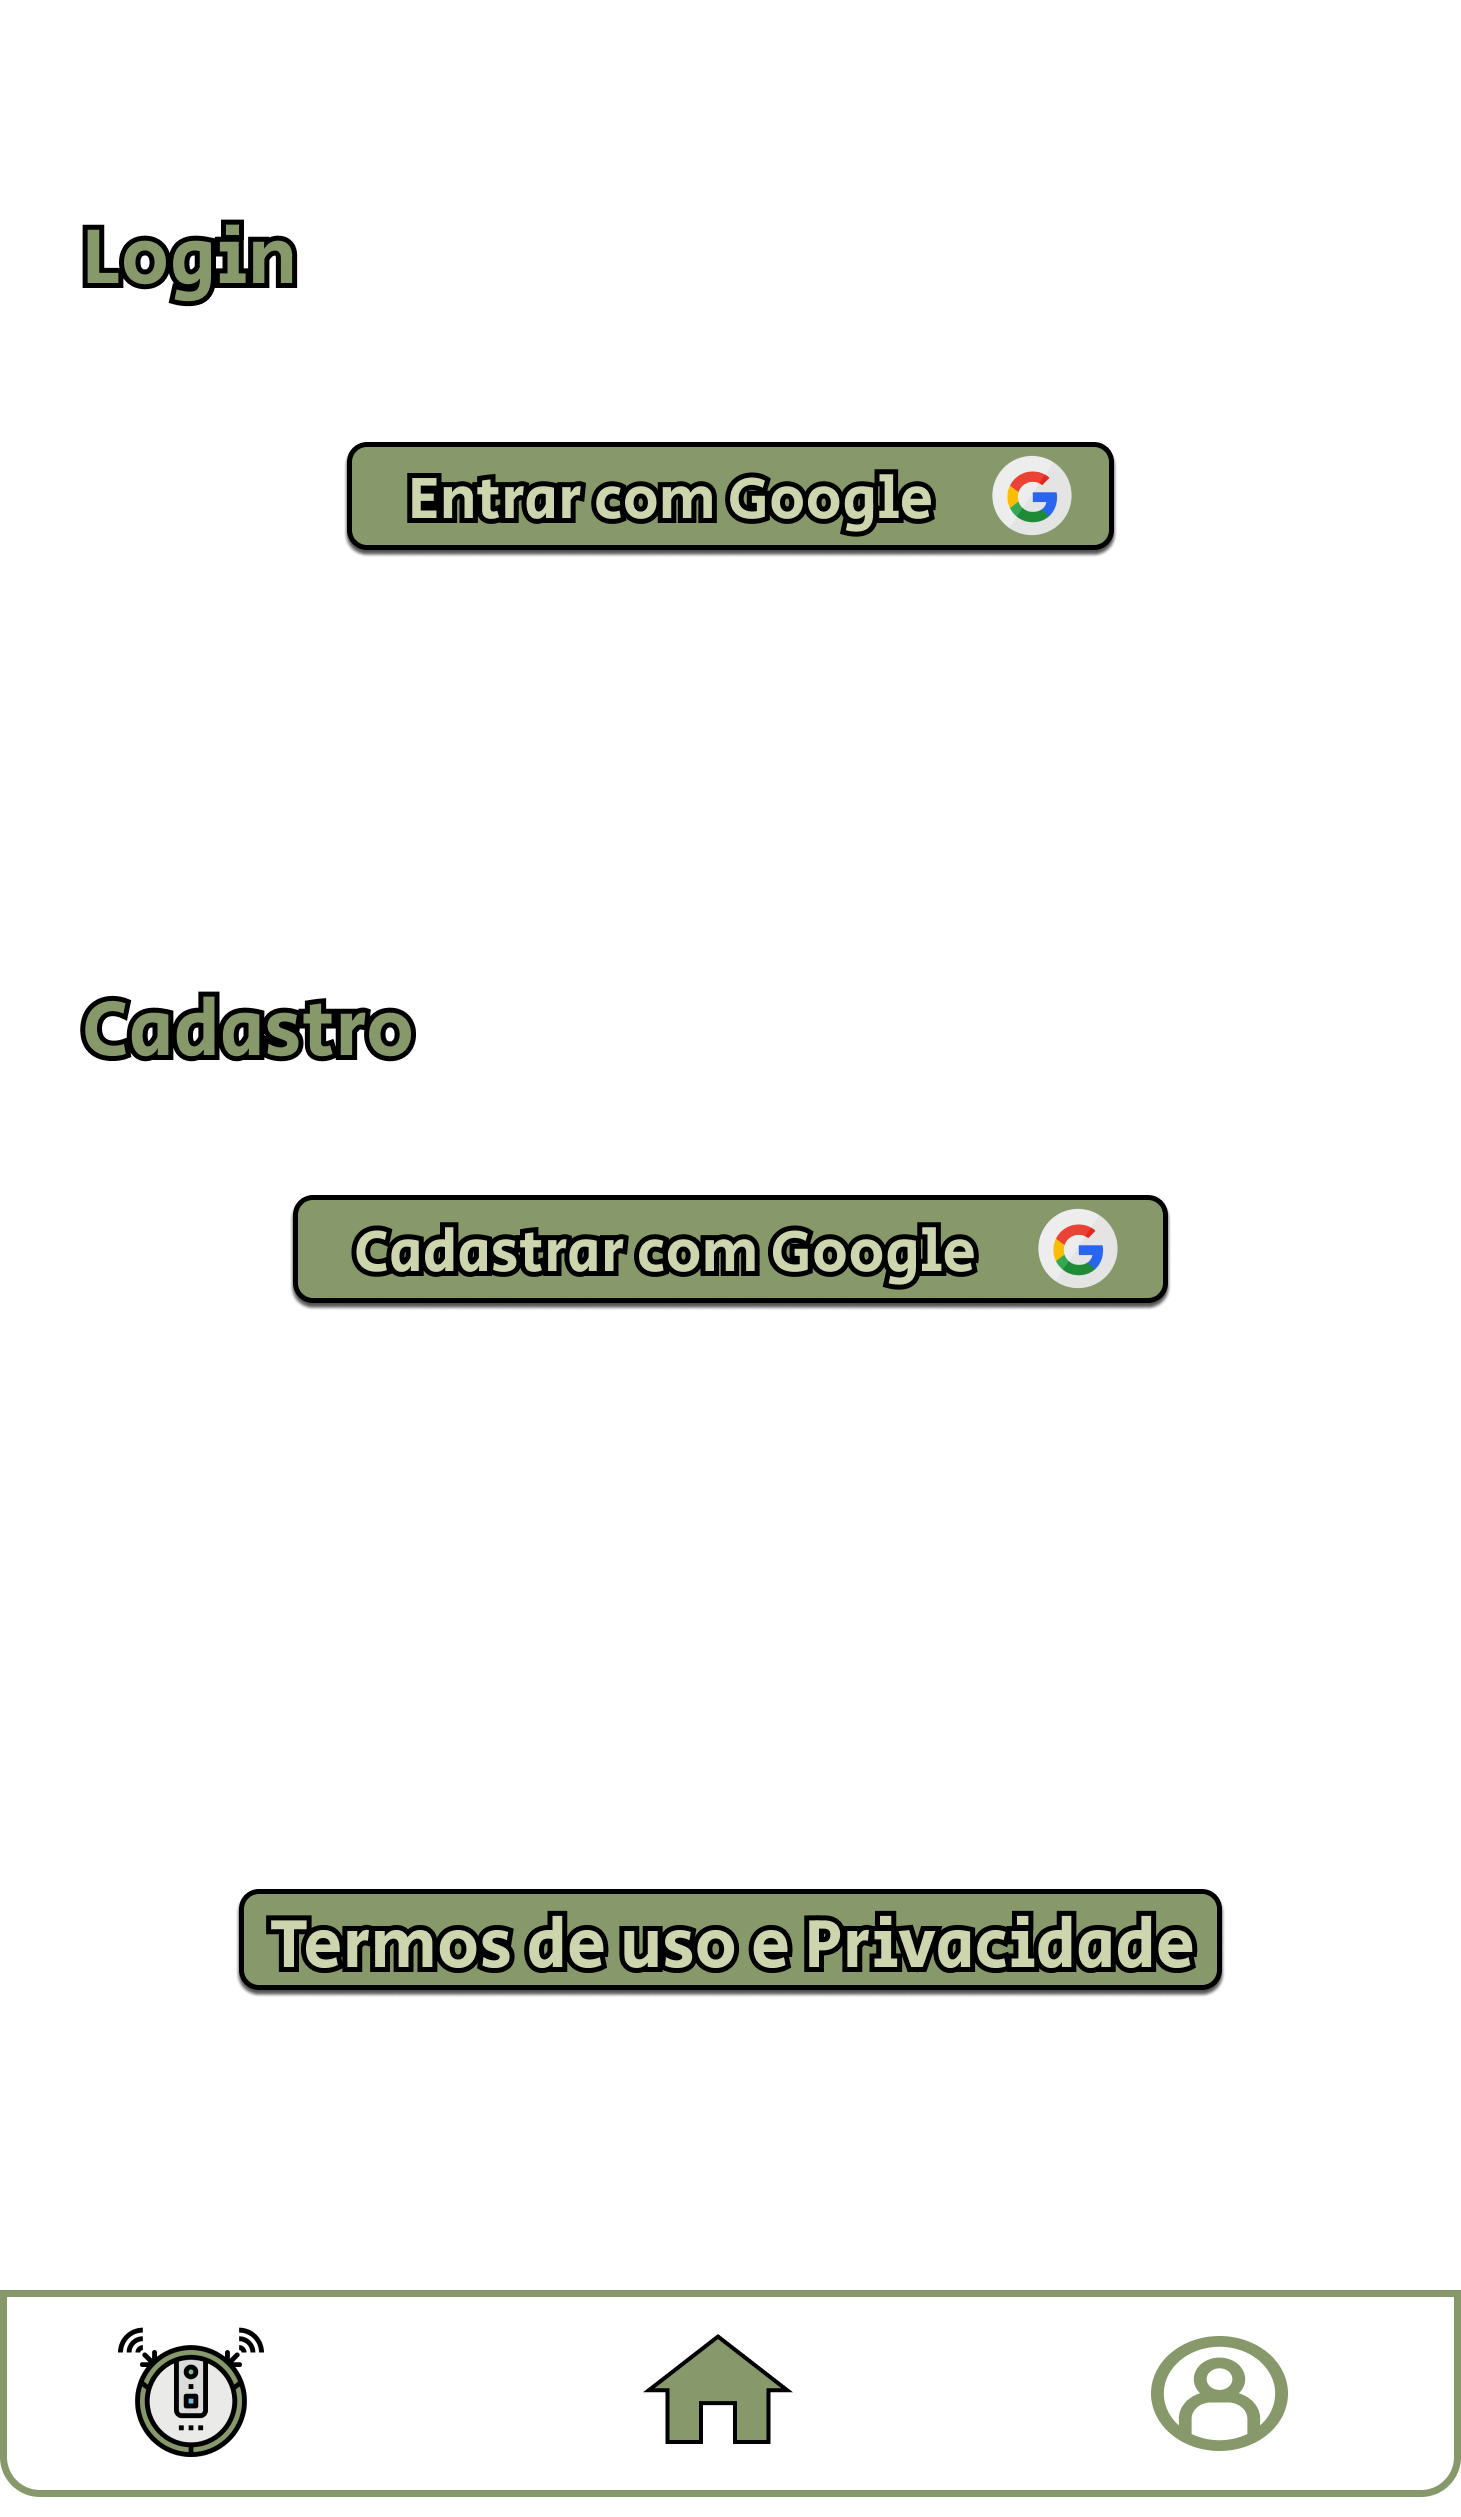
\includegraphics[height=10.0cm]{figuras/Mobile/Mob 1 - Login.png}}
\caption{Tela de Cadastro e Login}
\end{figure}

\subsection{Tela Inicial sem conexões}
\begin{figure}[H]
\centering
\frame{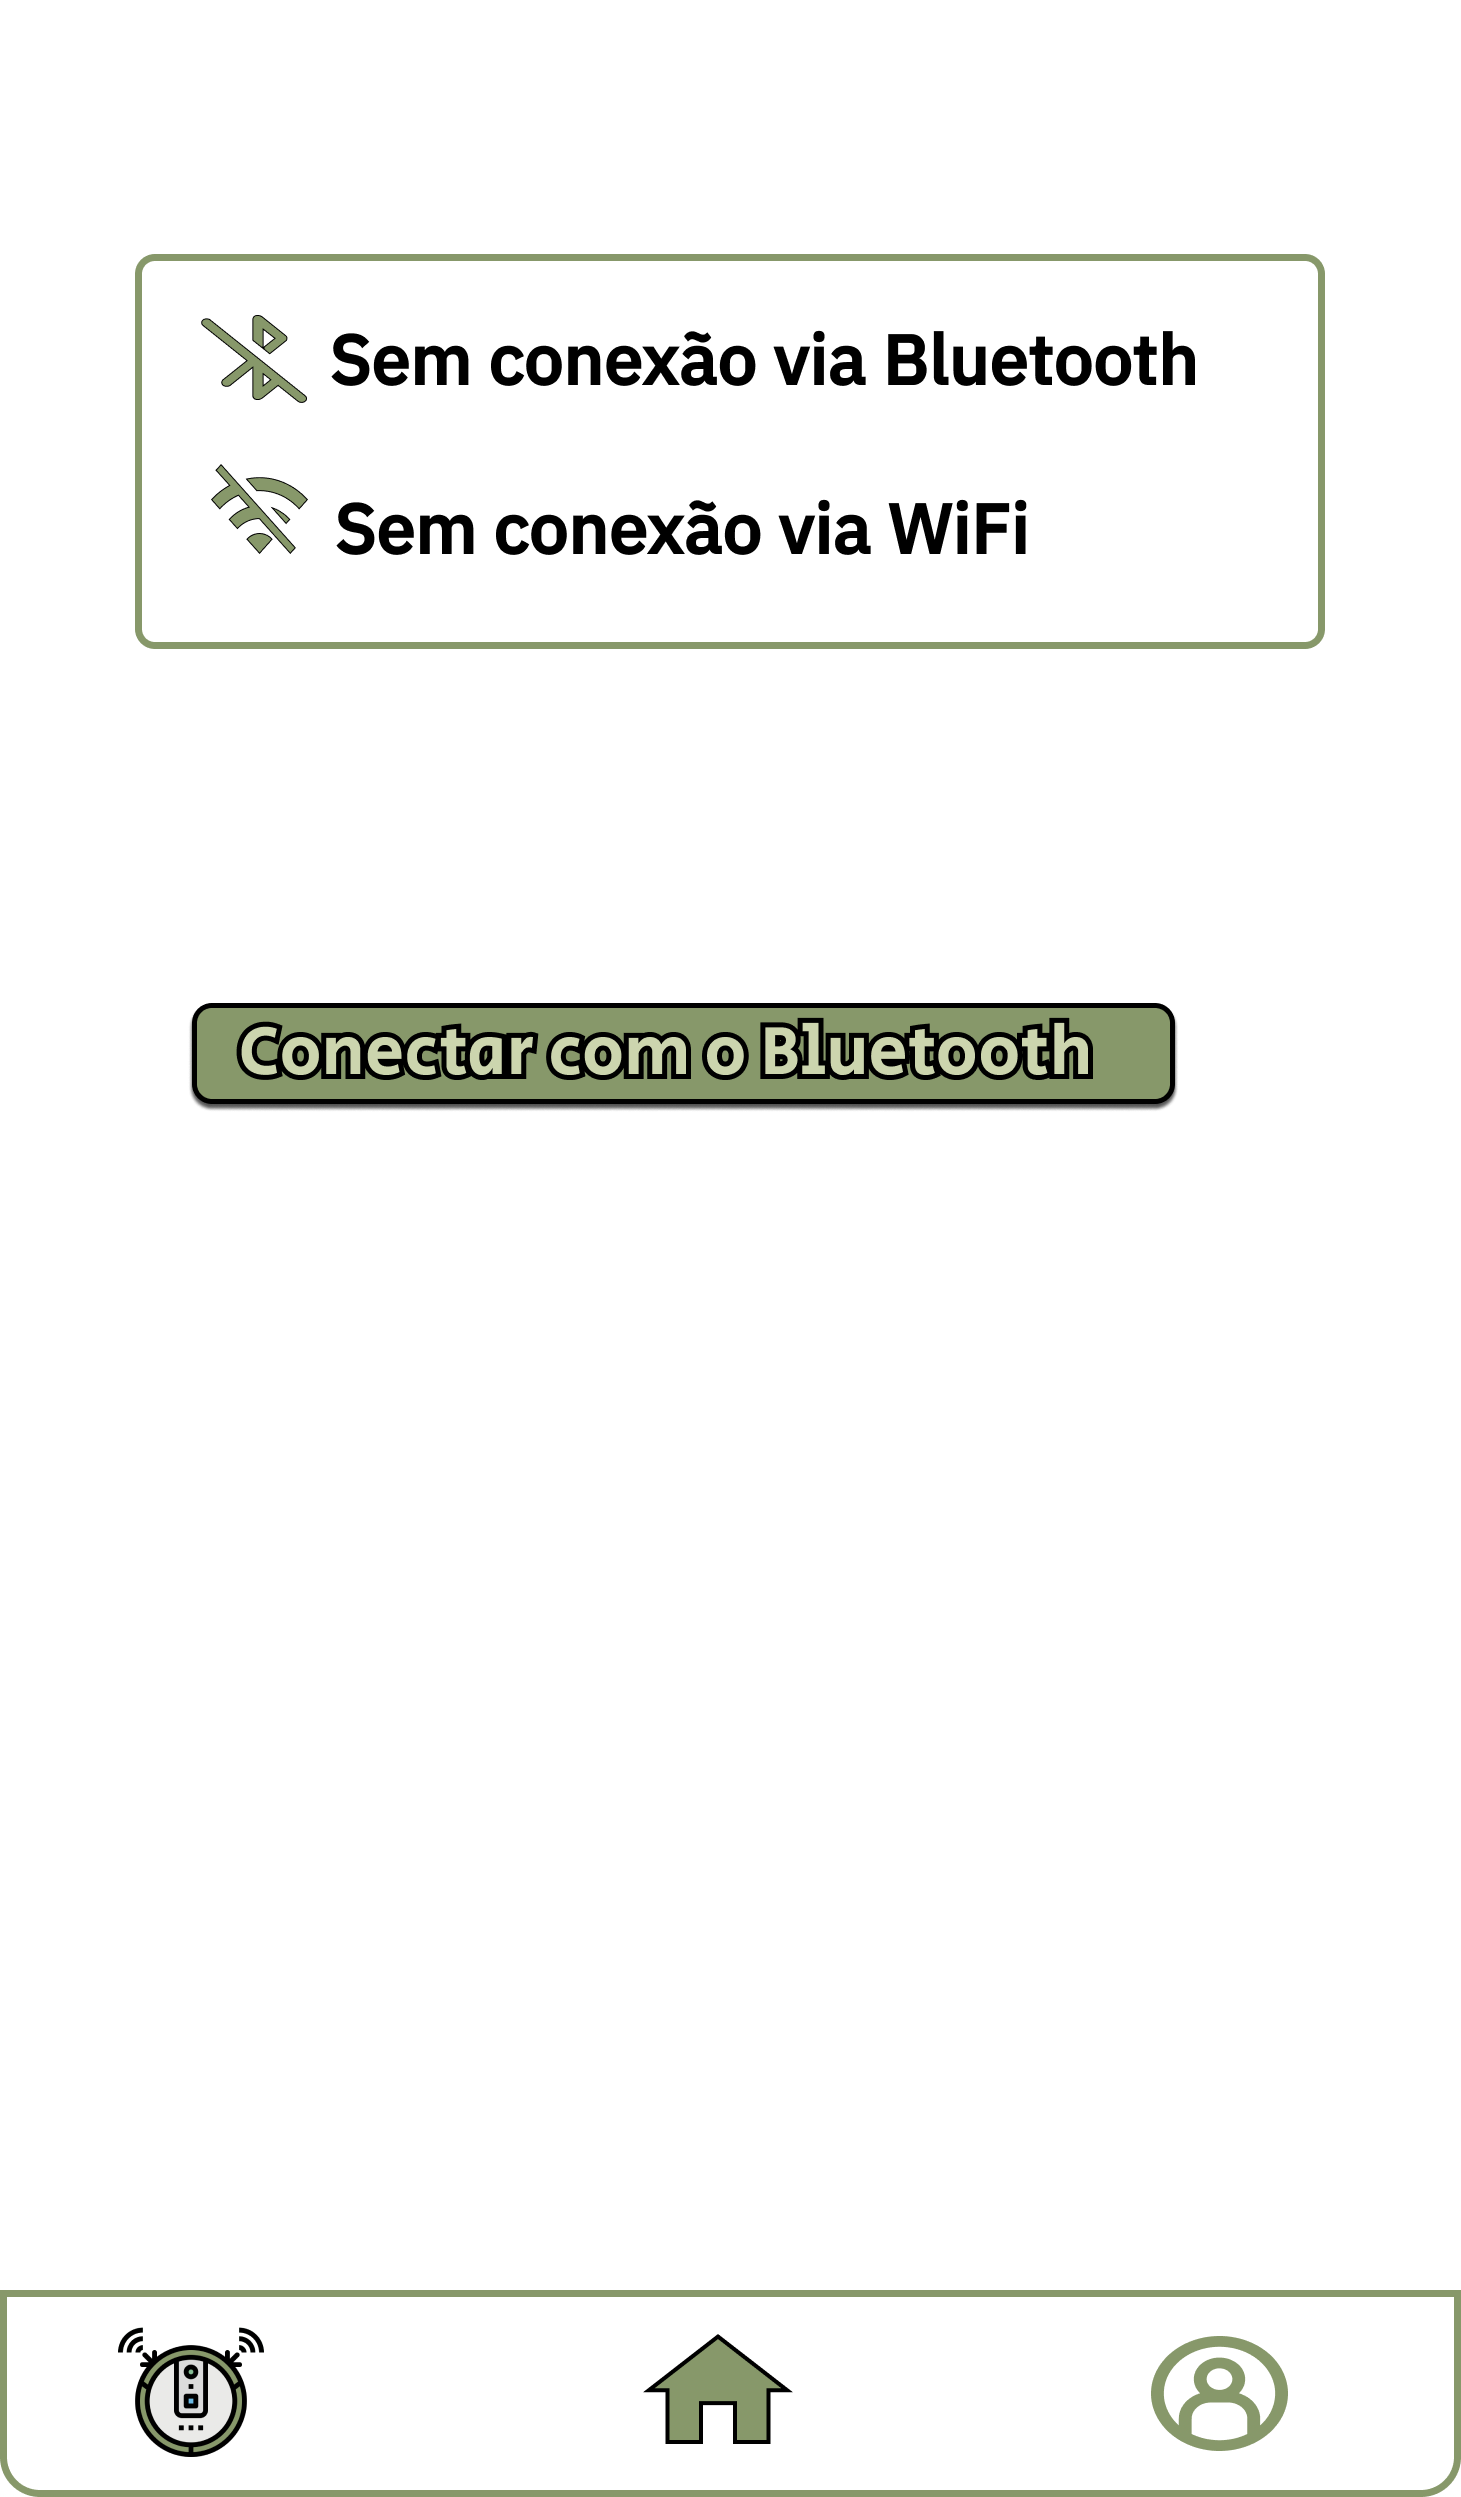
\includegraphics[height=8.5cm]{figuras/Mobile/Mob 2 - Sem conexoes.png}}
\caption{Tela Inicial sem conexões }
\end{figure}

\subsection{Tela Inicial conectada ao Bluetooth}
\begin{figure}[H]
\centering
\frame{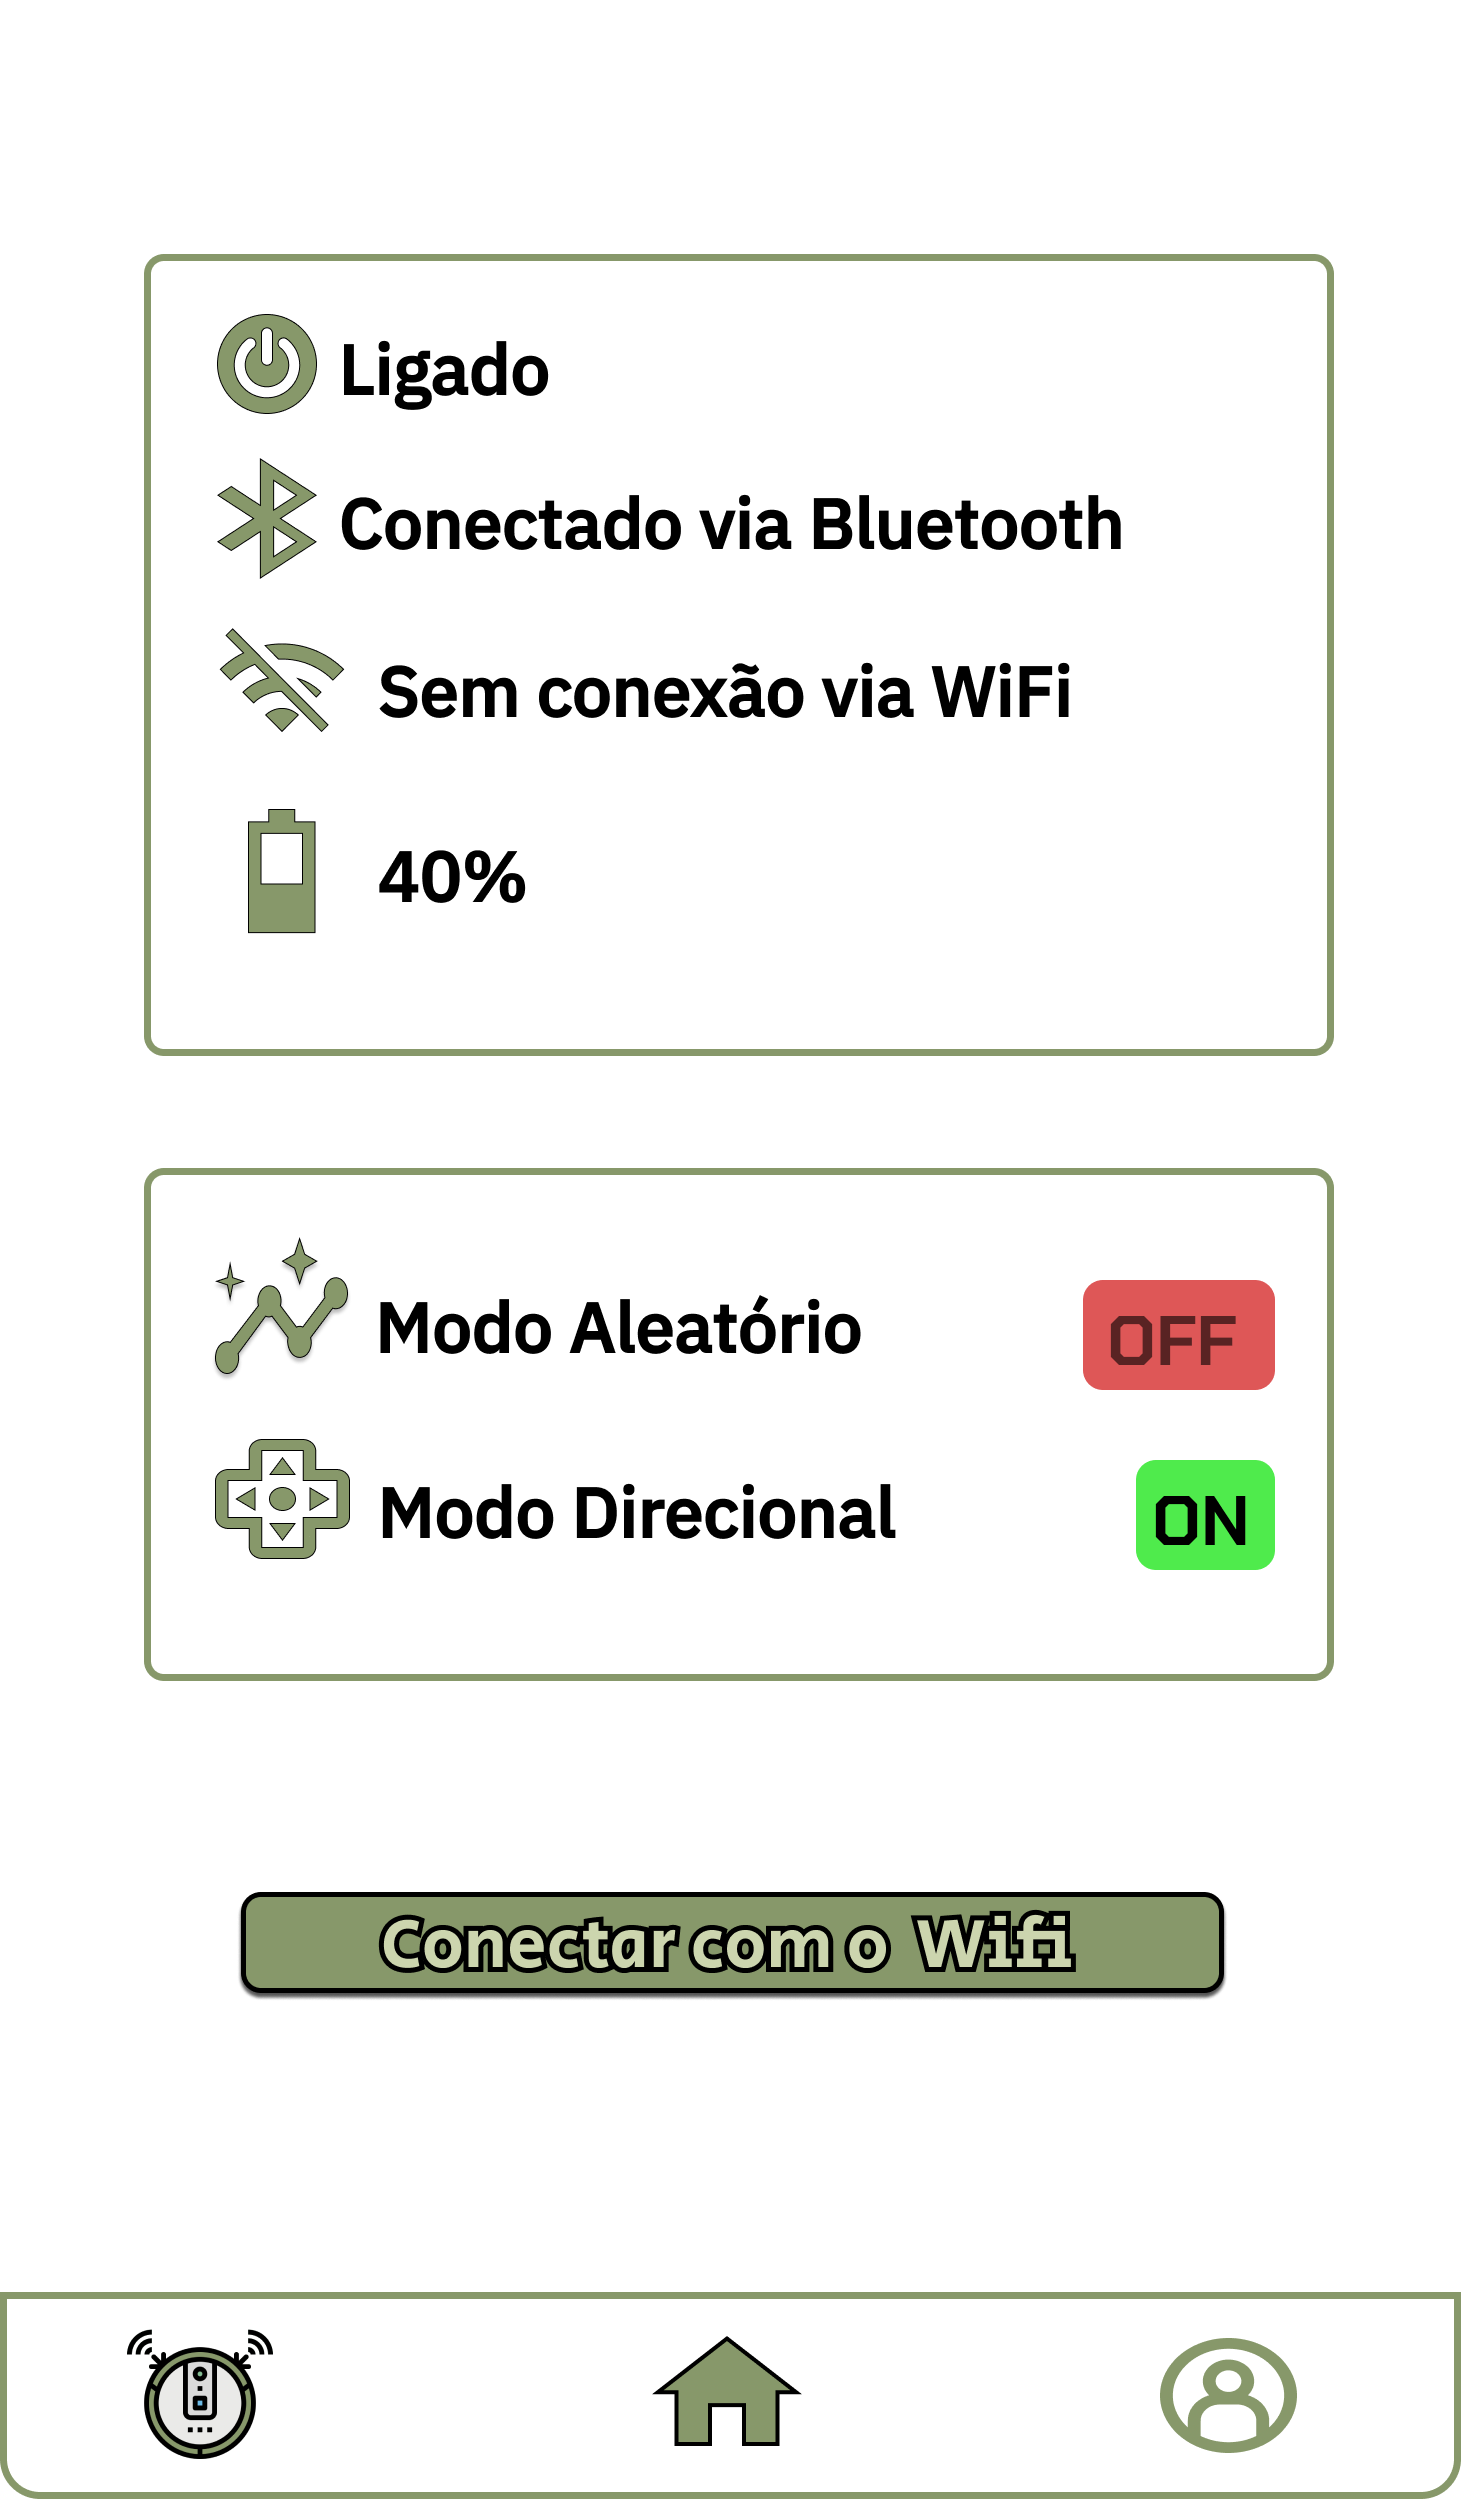
\includegraphics[height=8.5cm]{figuras/Mobile/Mob 3 - Status 1.png}}
\caption{Tela Inicial conectada ao Bluetooth}
\end{figure}

\subsection{Tela de Perfil}
\begin{figure}[H]
\centering
\frame{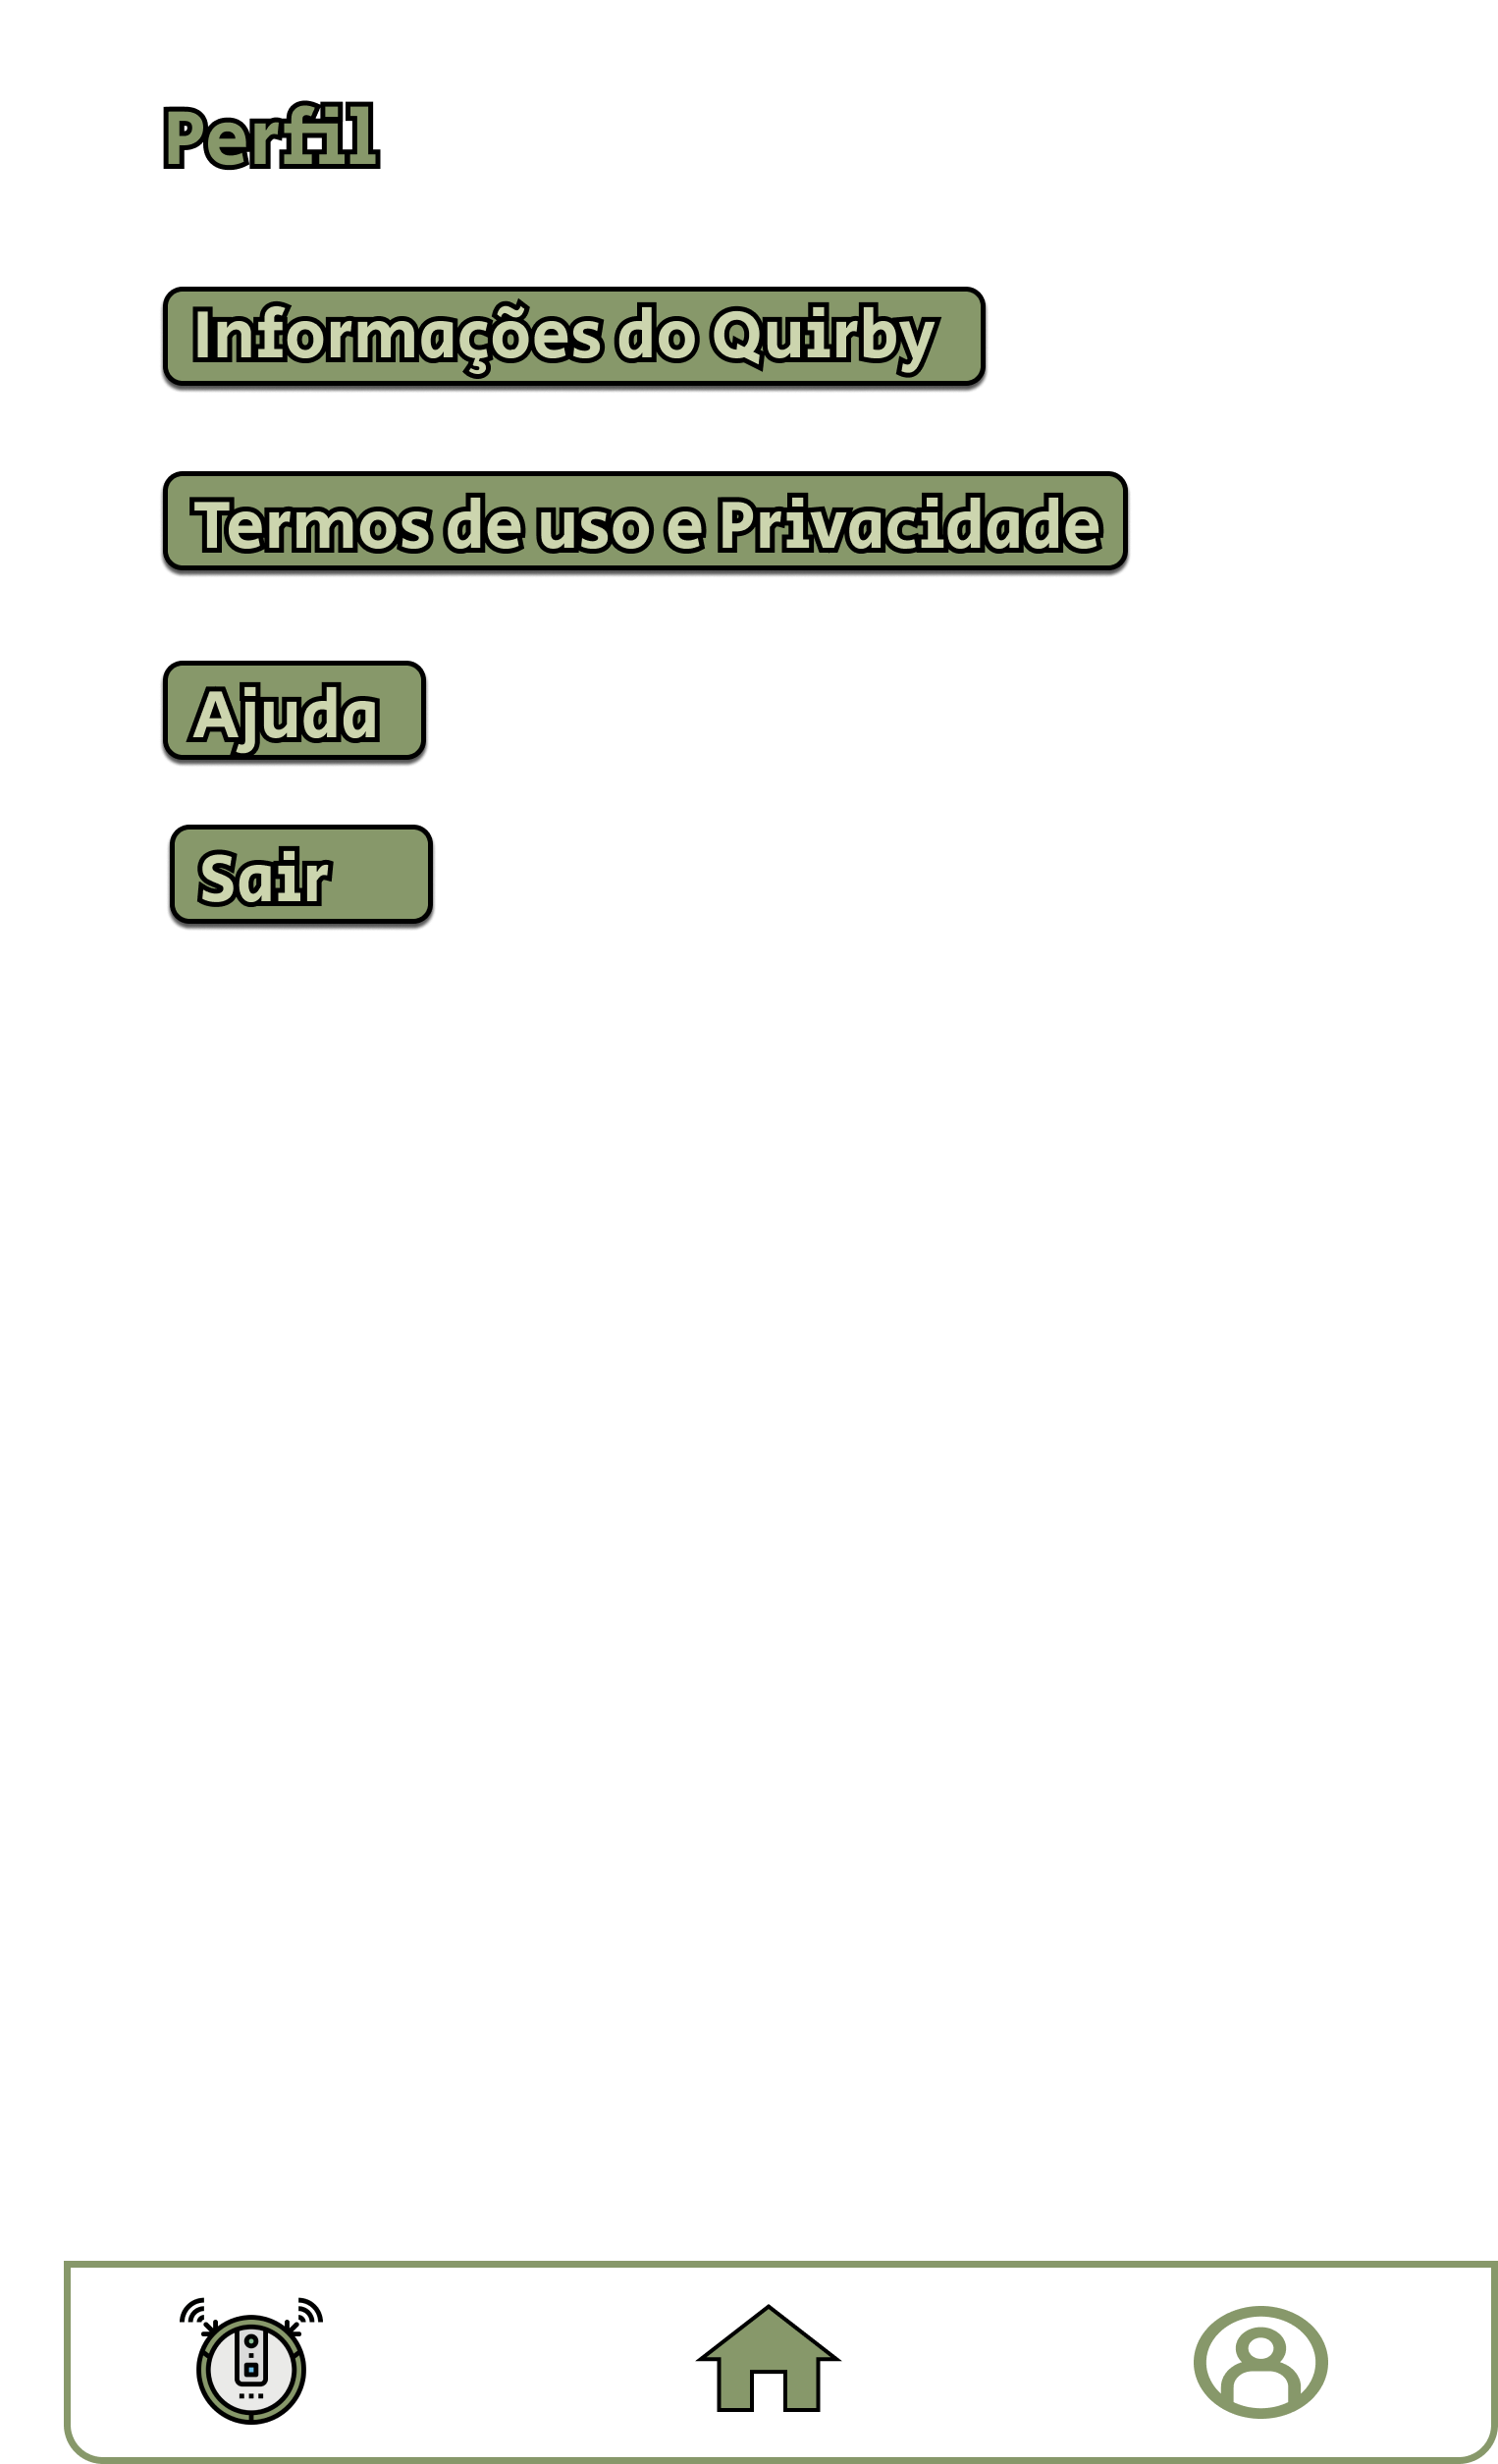
\includegraphics[height=8.5cm]{figuras/Mobile/Mob 4 - Perfil.png}}
\caption{Tela de Perfil}
\end{figure}

\subsection{Tela de Informações do Quirby}
\begin{figure}[H]
\centering
\frame{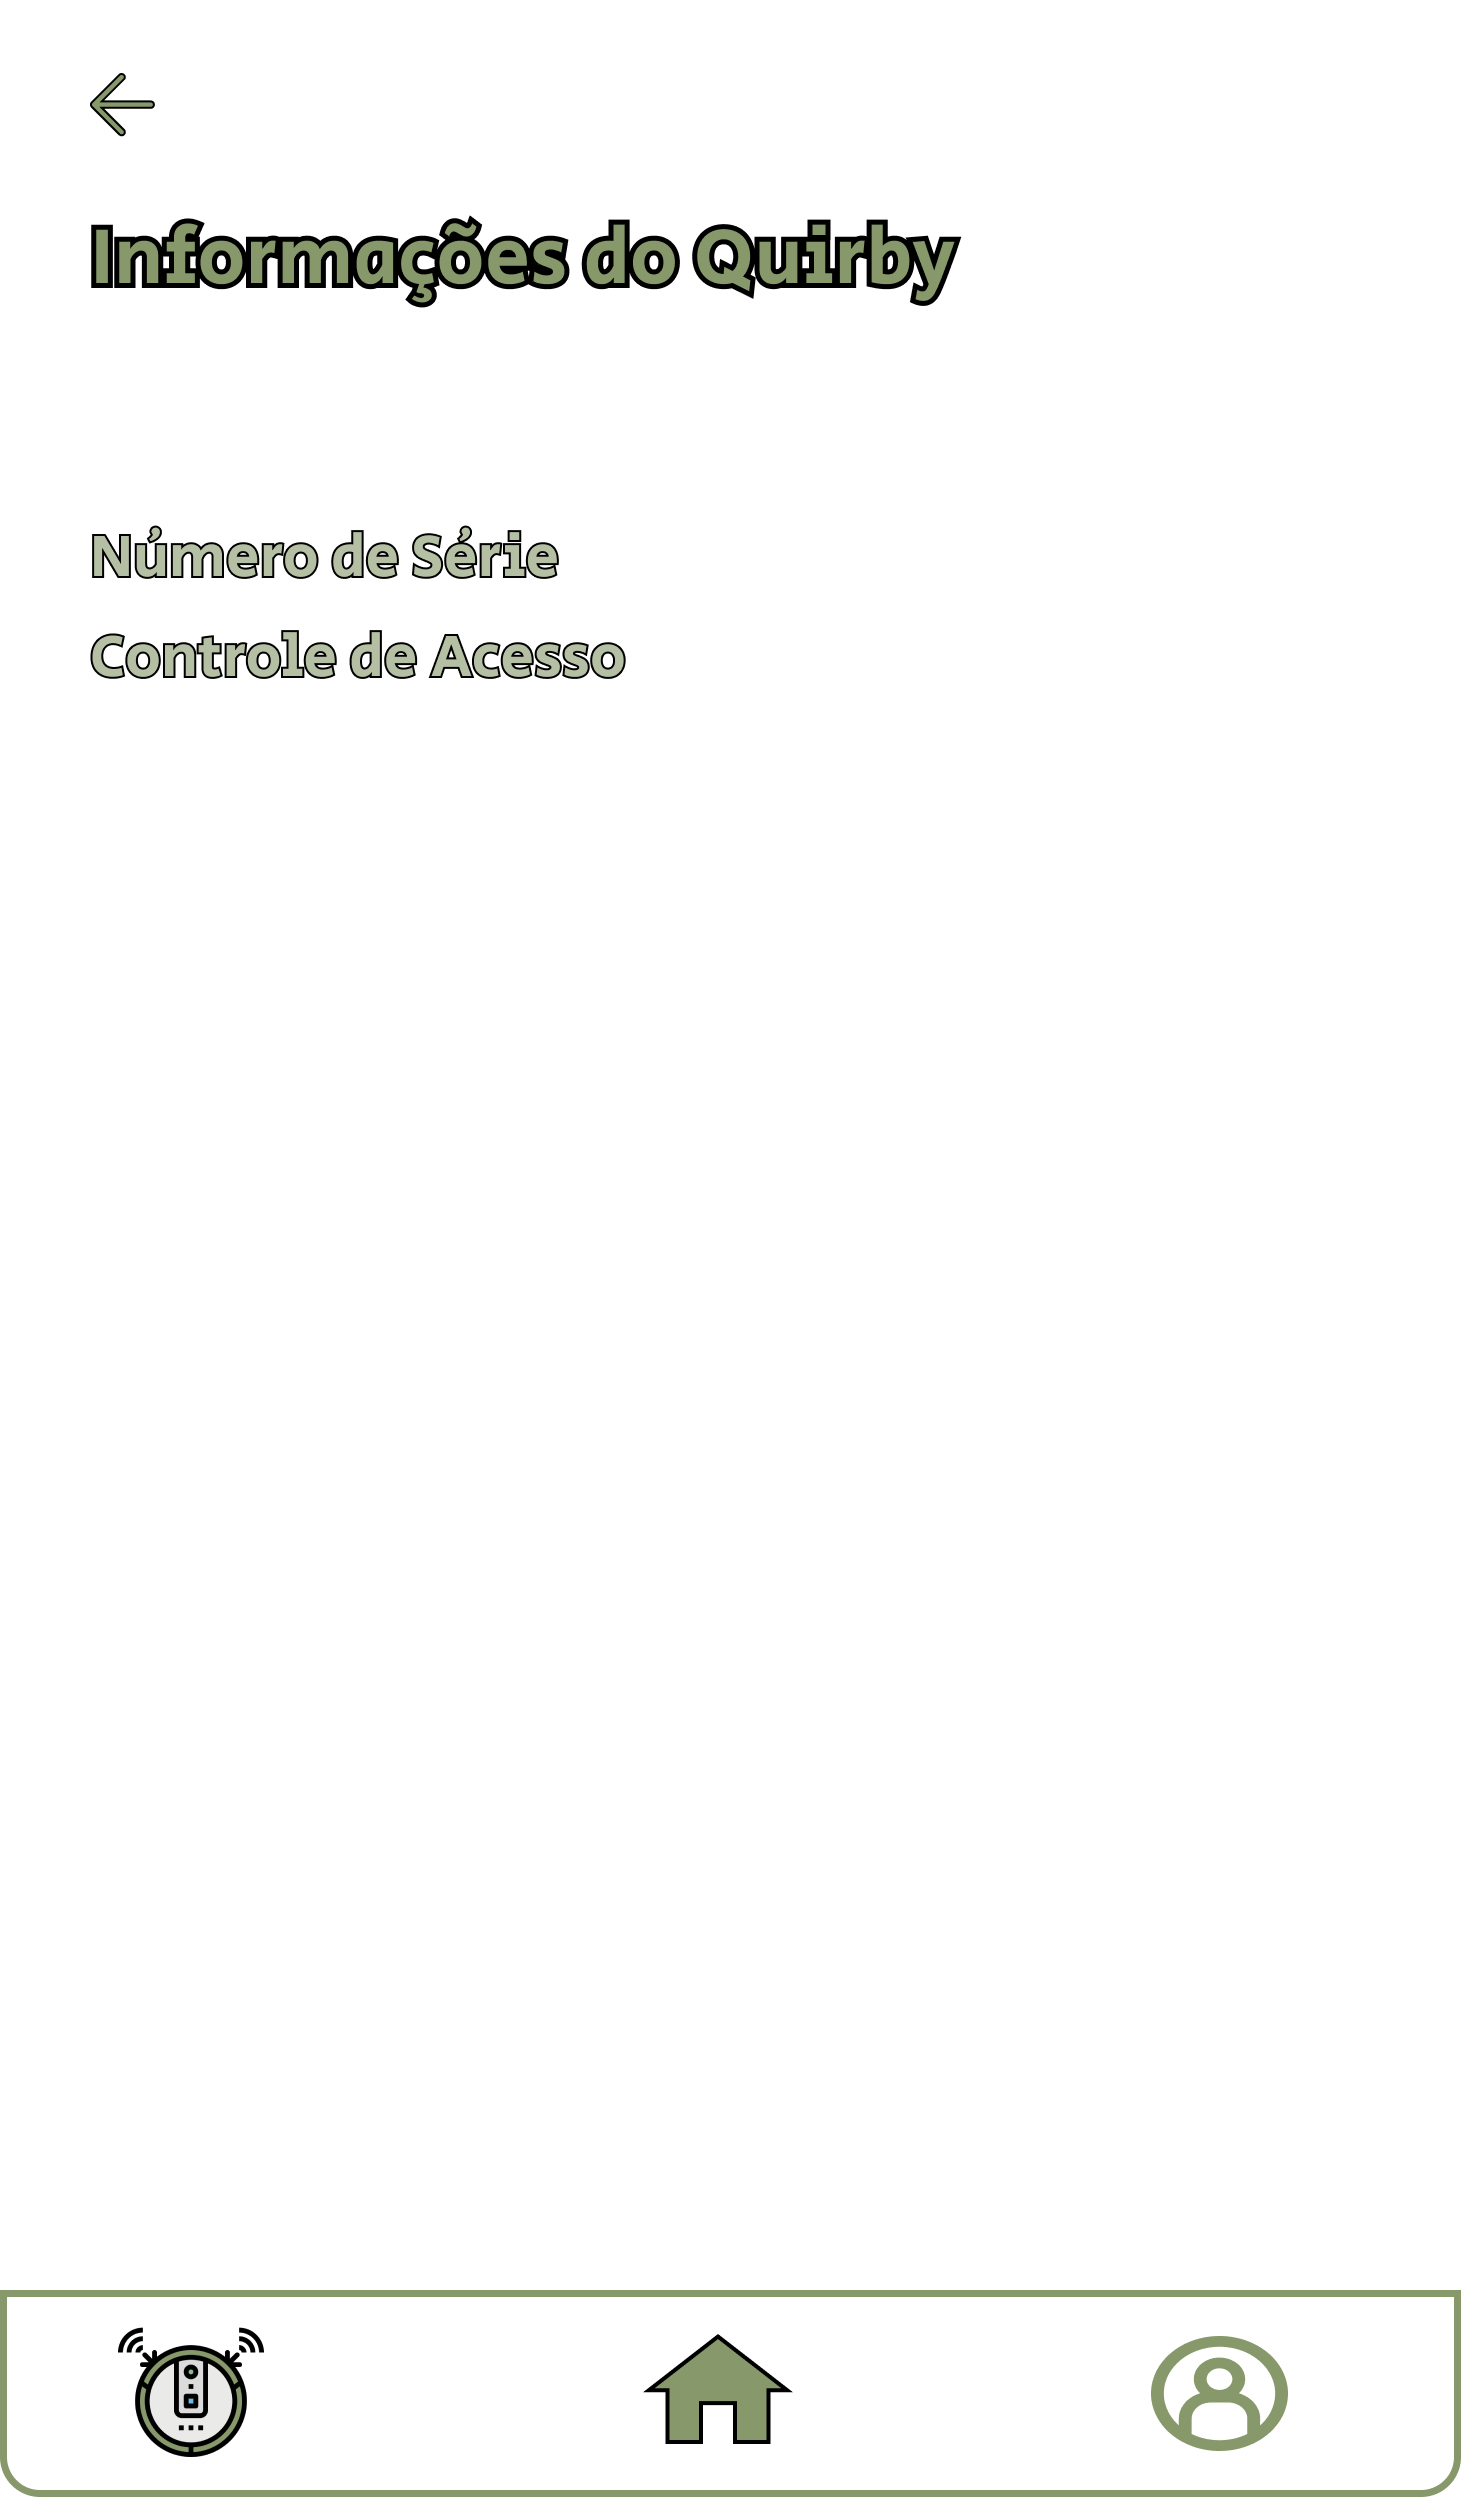
\includegraphics[height=8.5cm]{figuras/Mobile/Mob 5 - Informações do Quirby.png}}
\caption{Tela de Informações do Quirby}
\end{figure}

\subsection{Tela de Ajuda}
\begin{figure}[H]
\centering
\frame{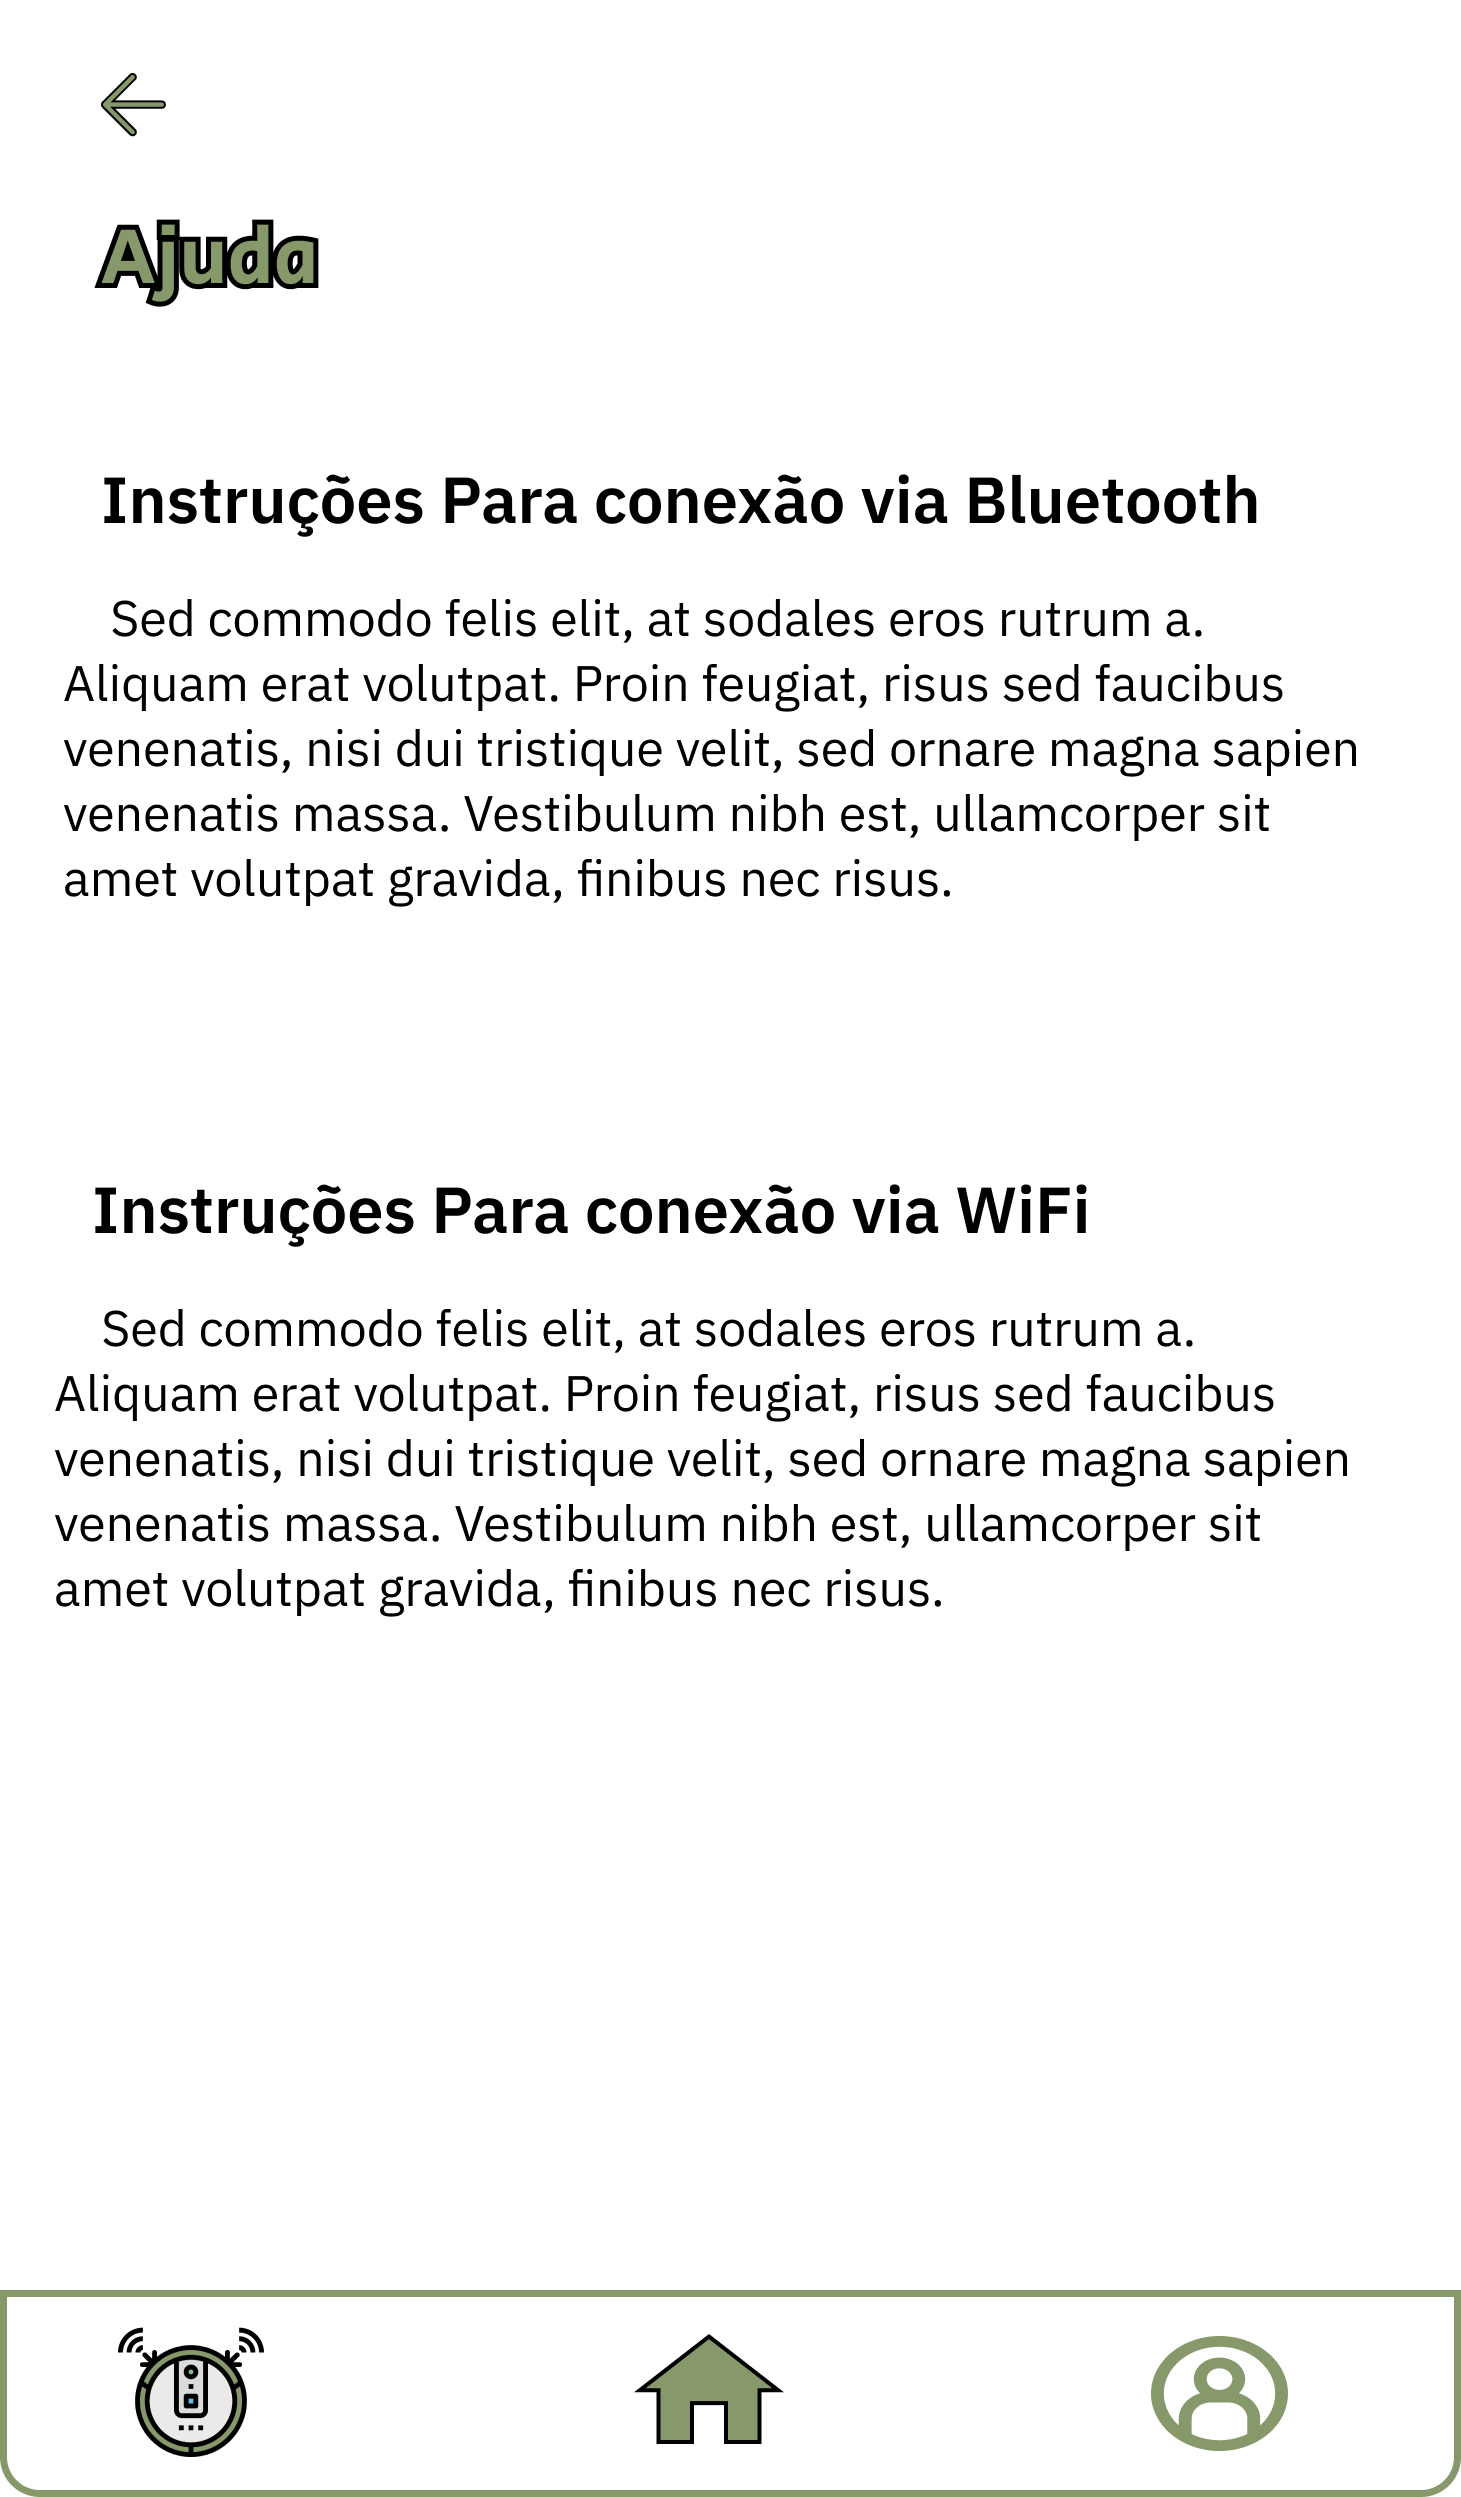
\includegraphics[height=8.5cm]{figuras/Mobile/Mob 6 - Ajuda.png}}
\caption{Tela de Ajuda}
\end{figure}

\subsection{Tela de Conectar ao WiFi}
\begin{figure}[H]
\centering
\frame{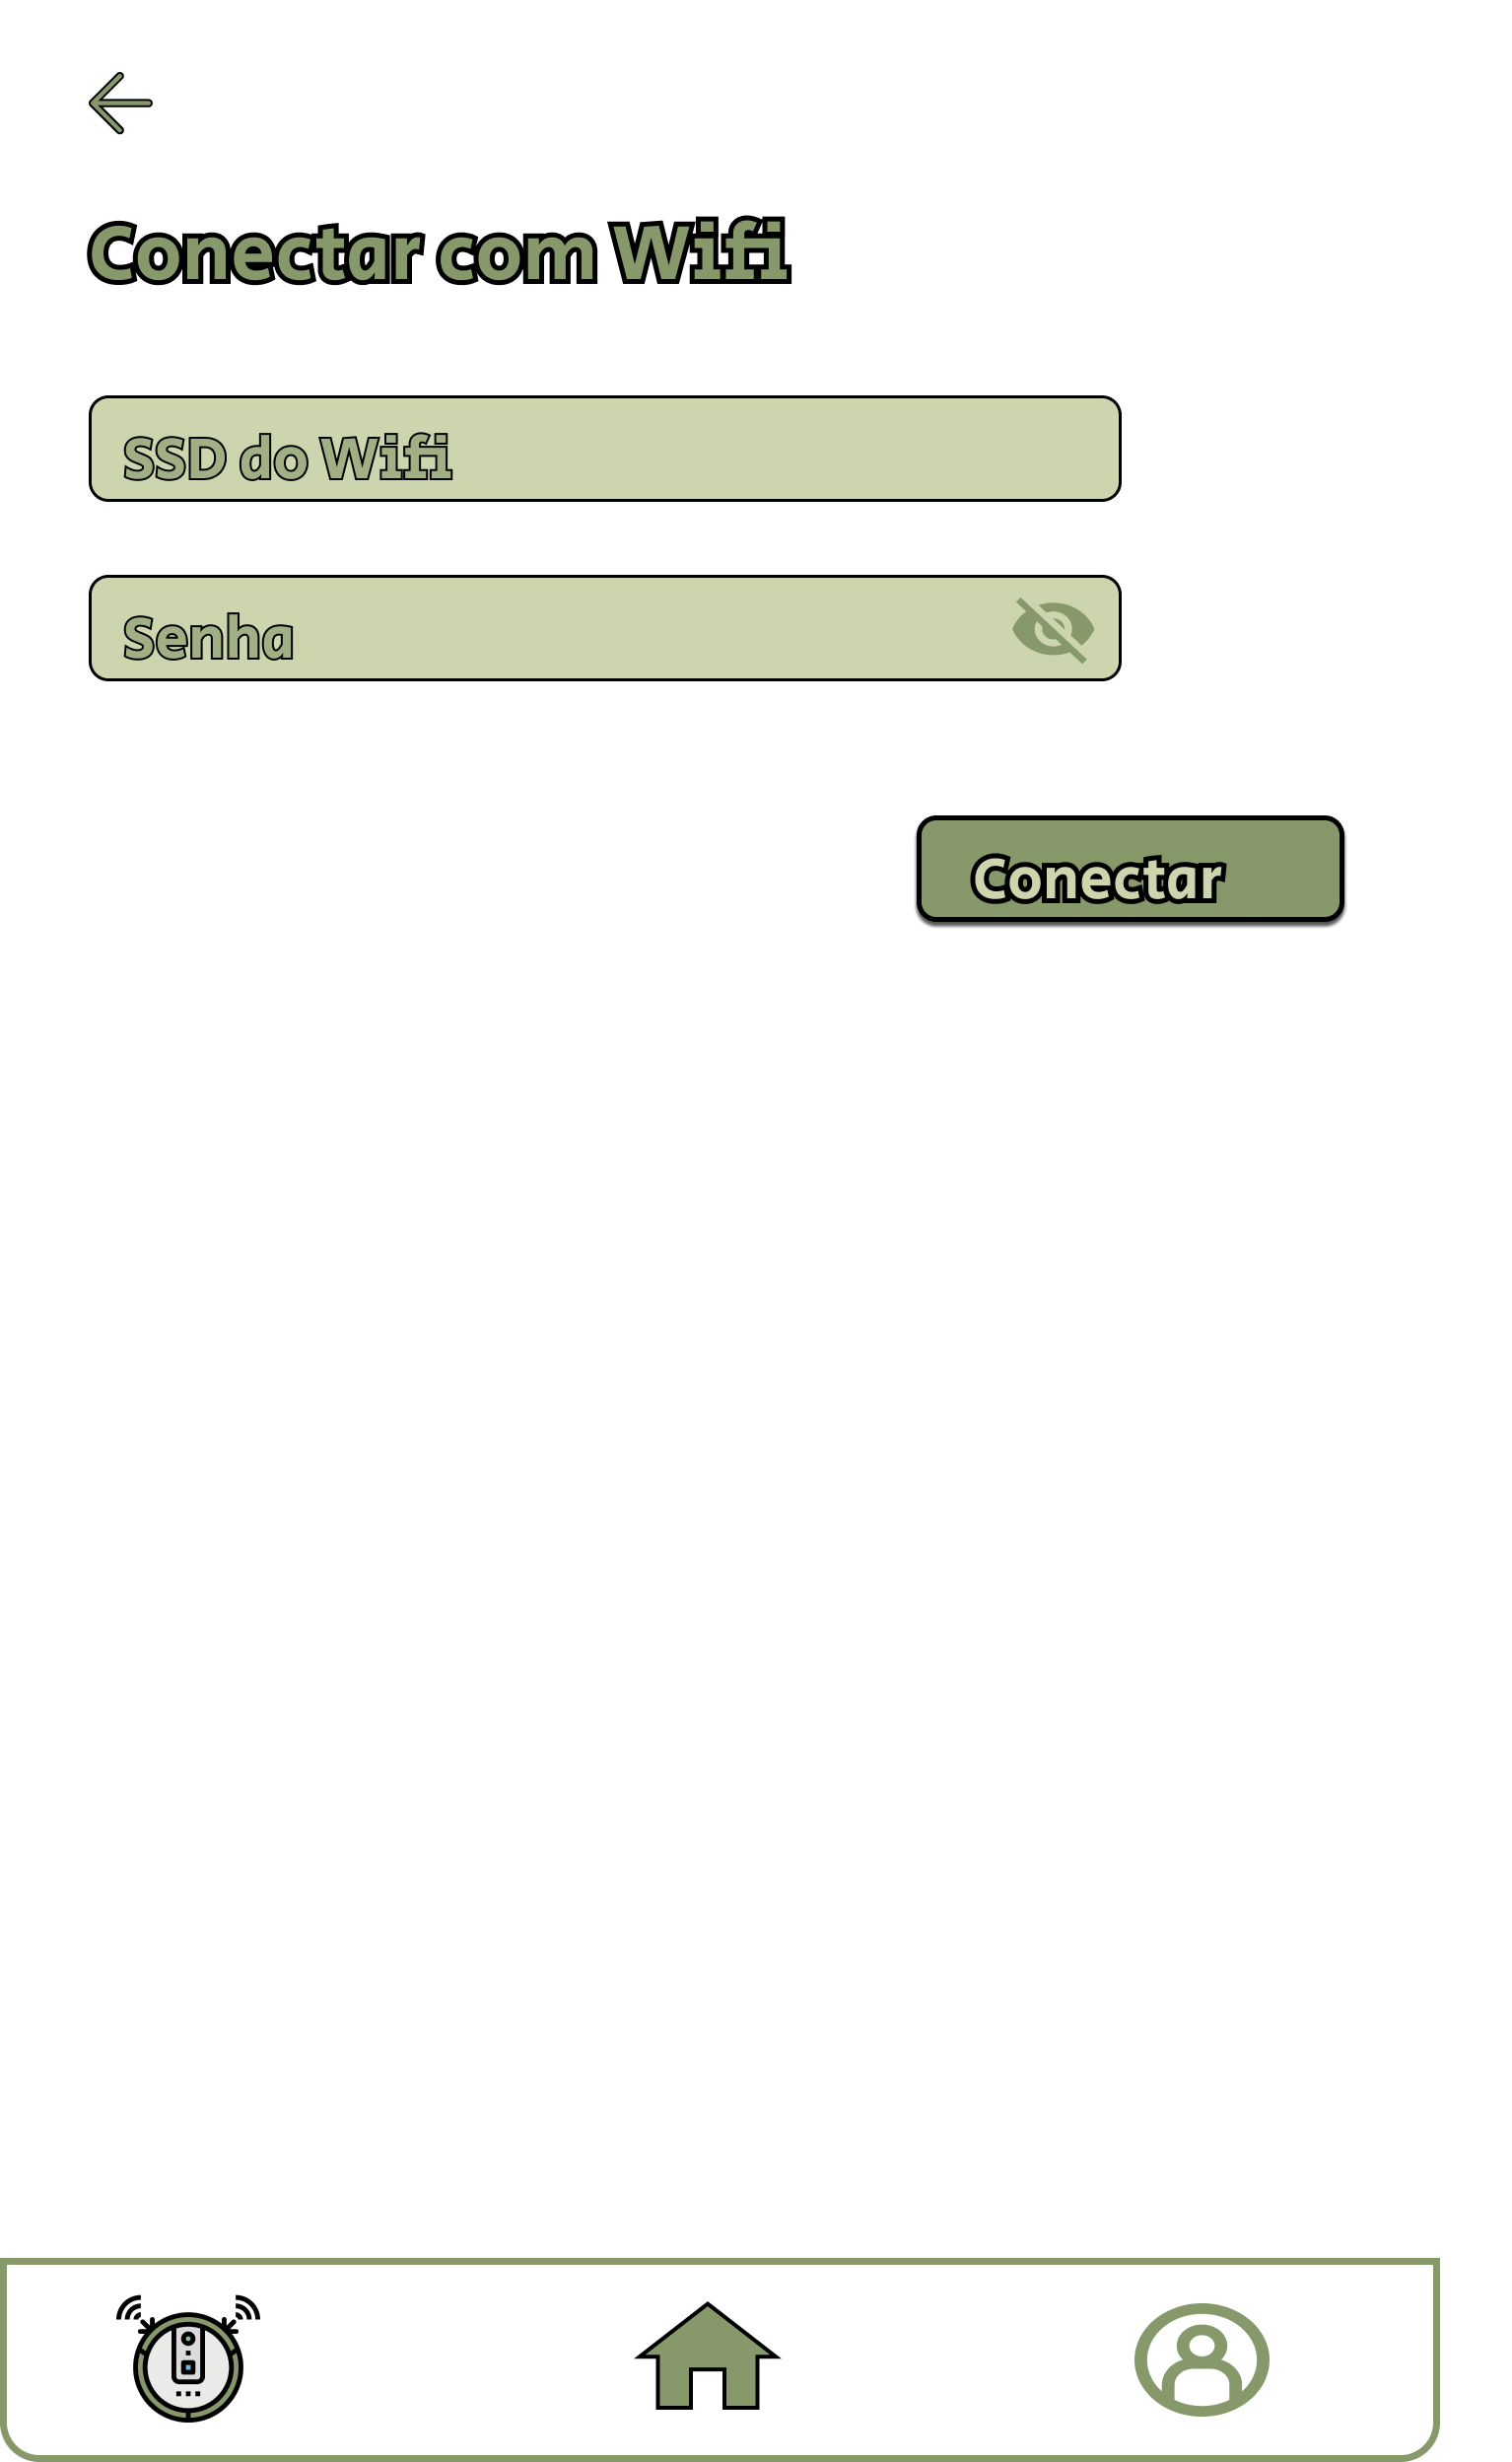
\includegraphics[height=8.5cm]{figuras/Mobile/Mod 7 - Conectar Wifi.png}}
\caption{Tela de Conectar ao WiFi}
\end{figure}

\subsection{Tela de Termos de Uso}
\begin{figure}[H]
\centering
\frame{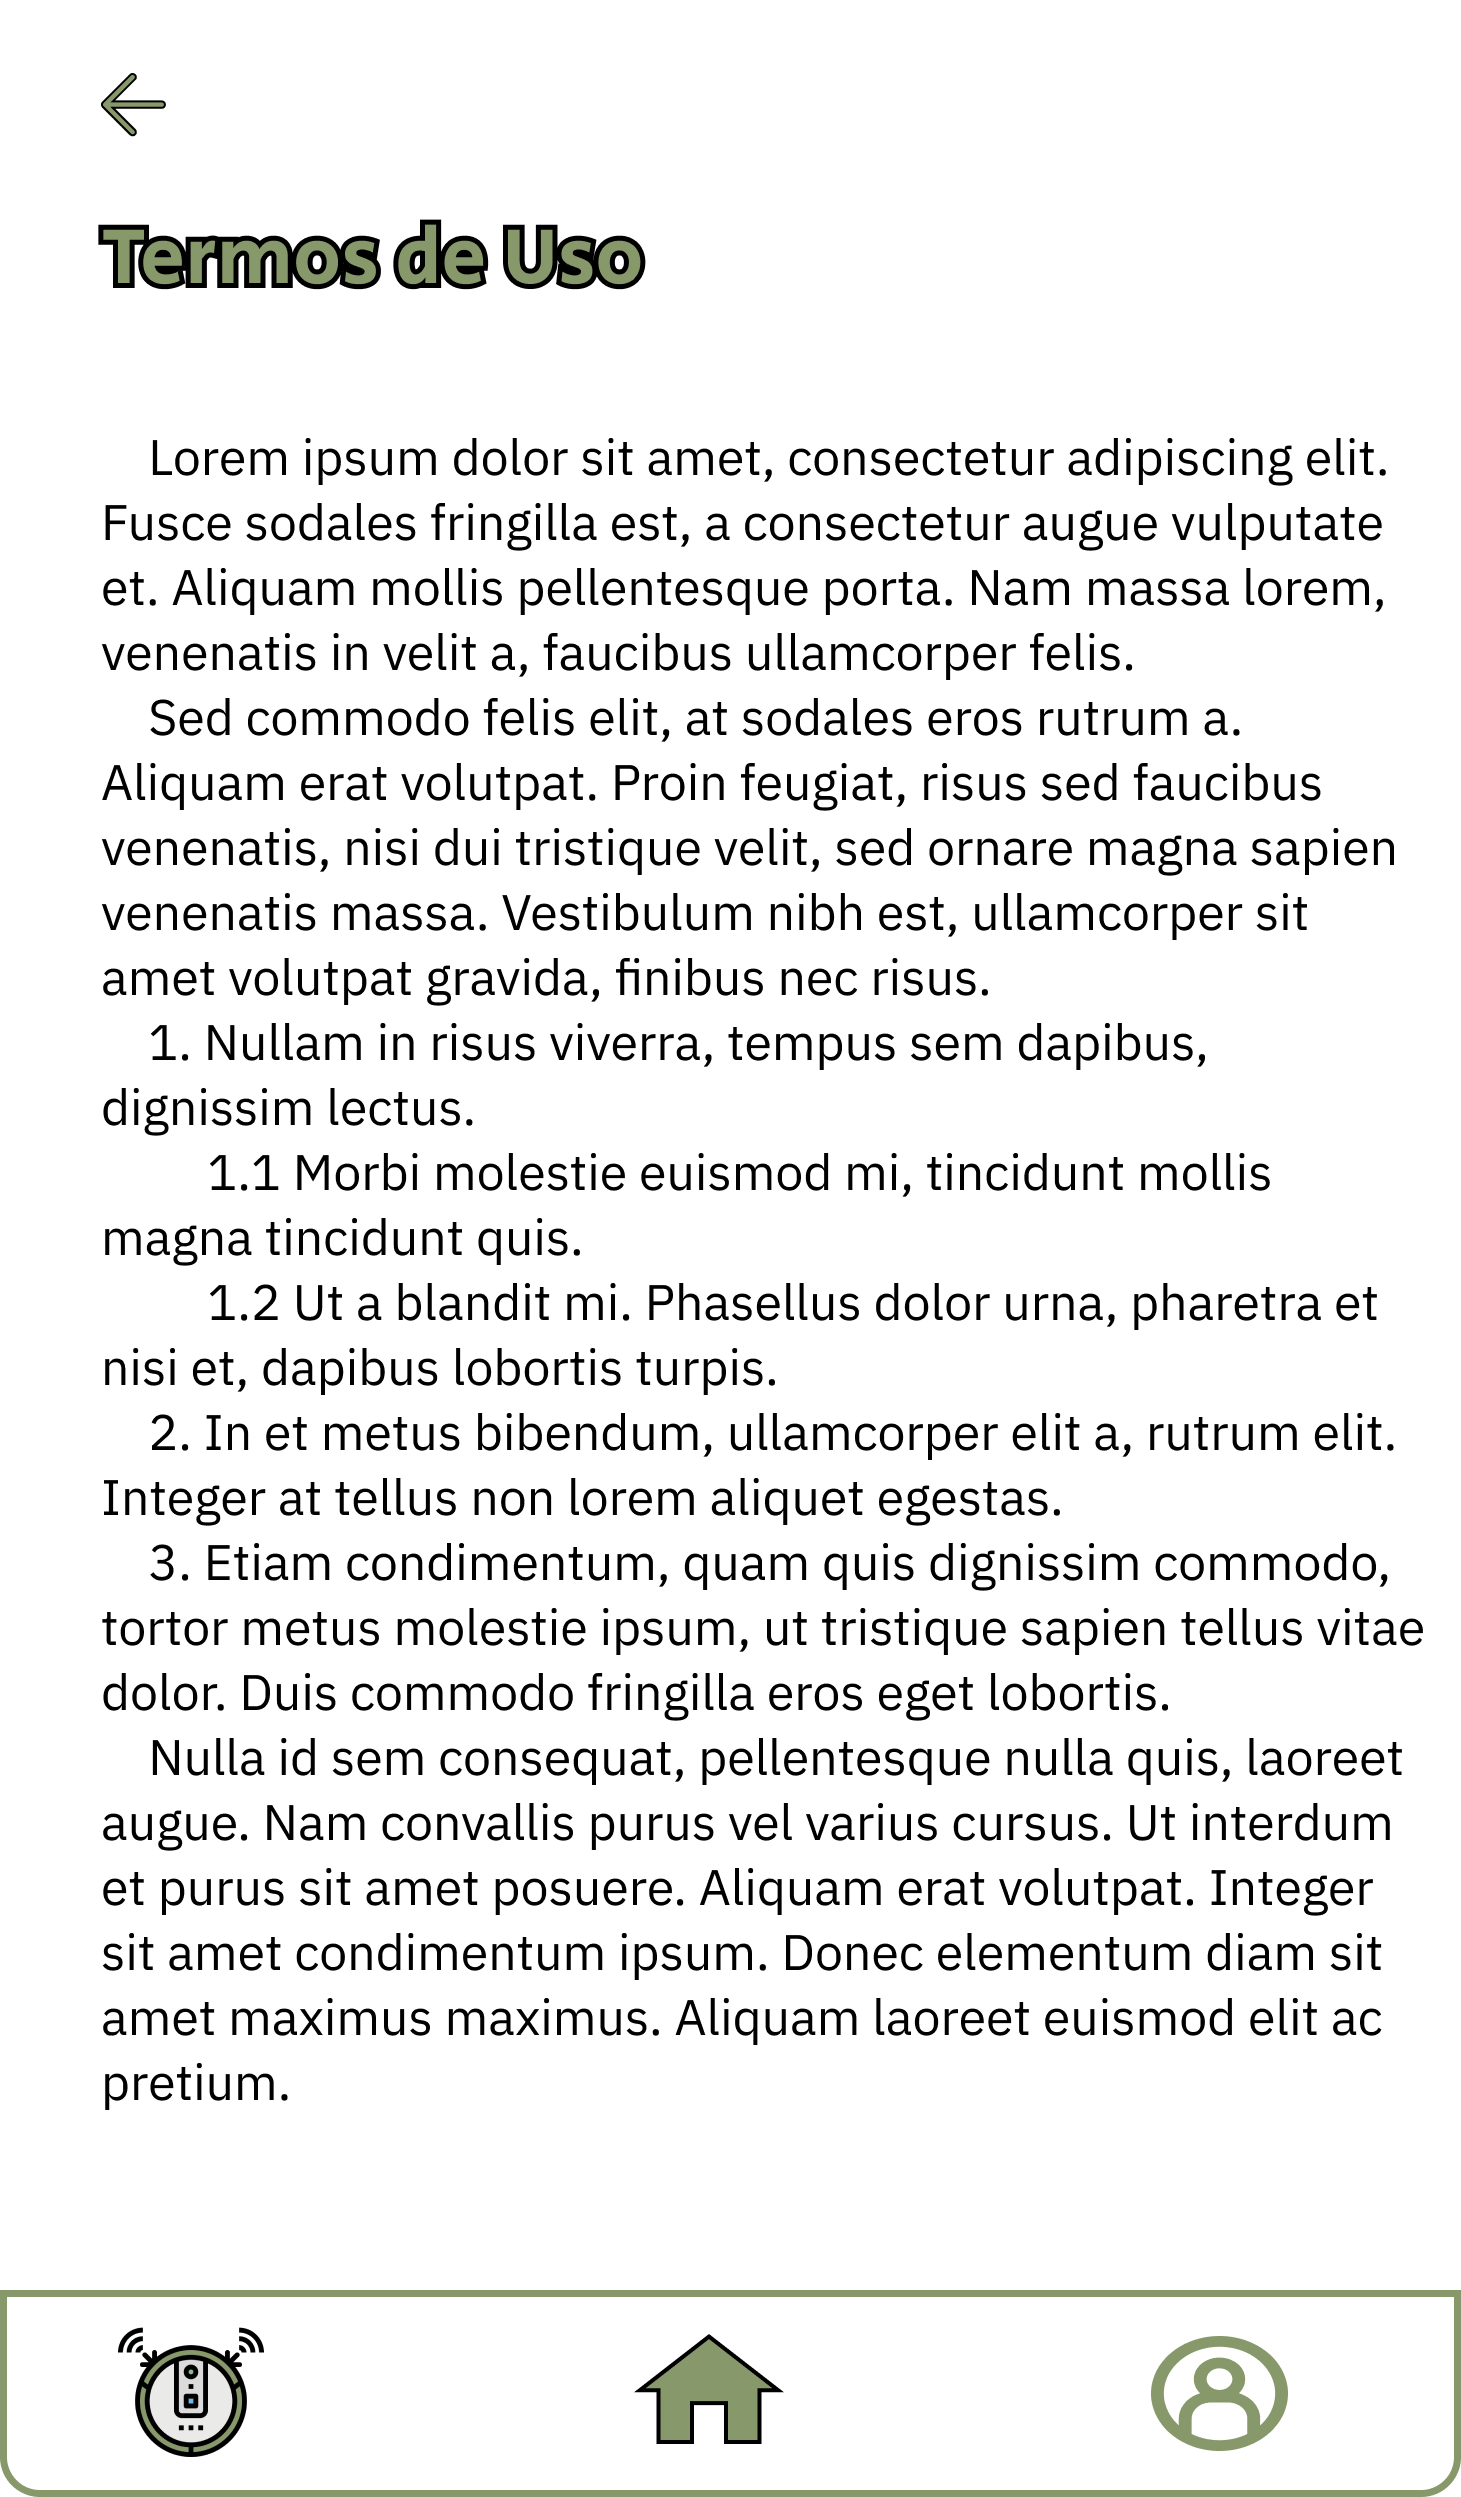
\includegraphics[height=8.5cm]{figuras/Mobile/uso.png}}
\caption{Tela de Termos de Uso}
\end{figure}

\subsection{Tela de Termos de Privacidade}
\begin{figure}[H]
\centering
\frame{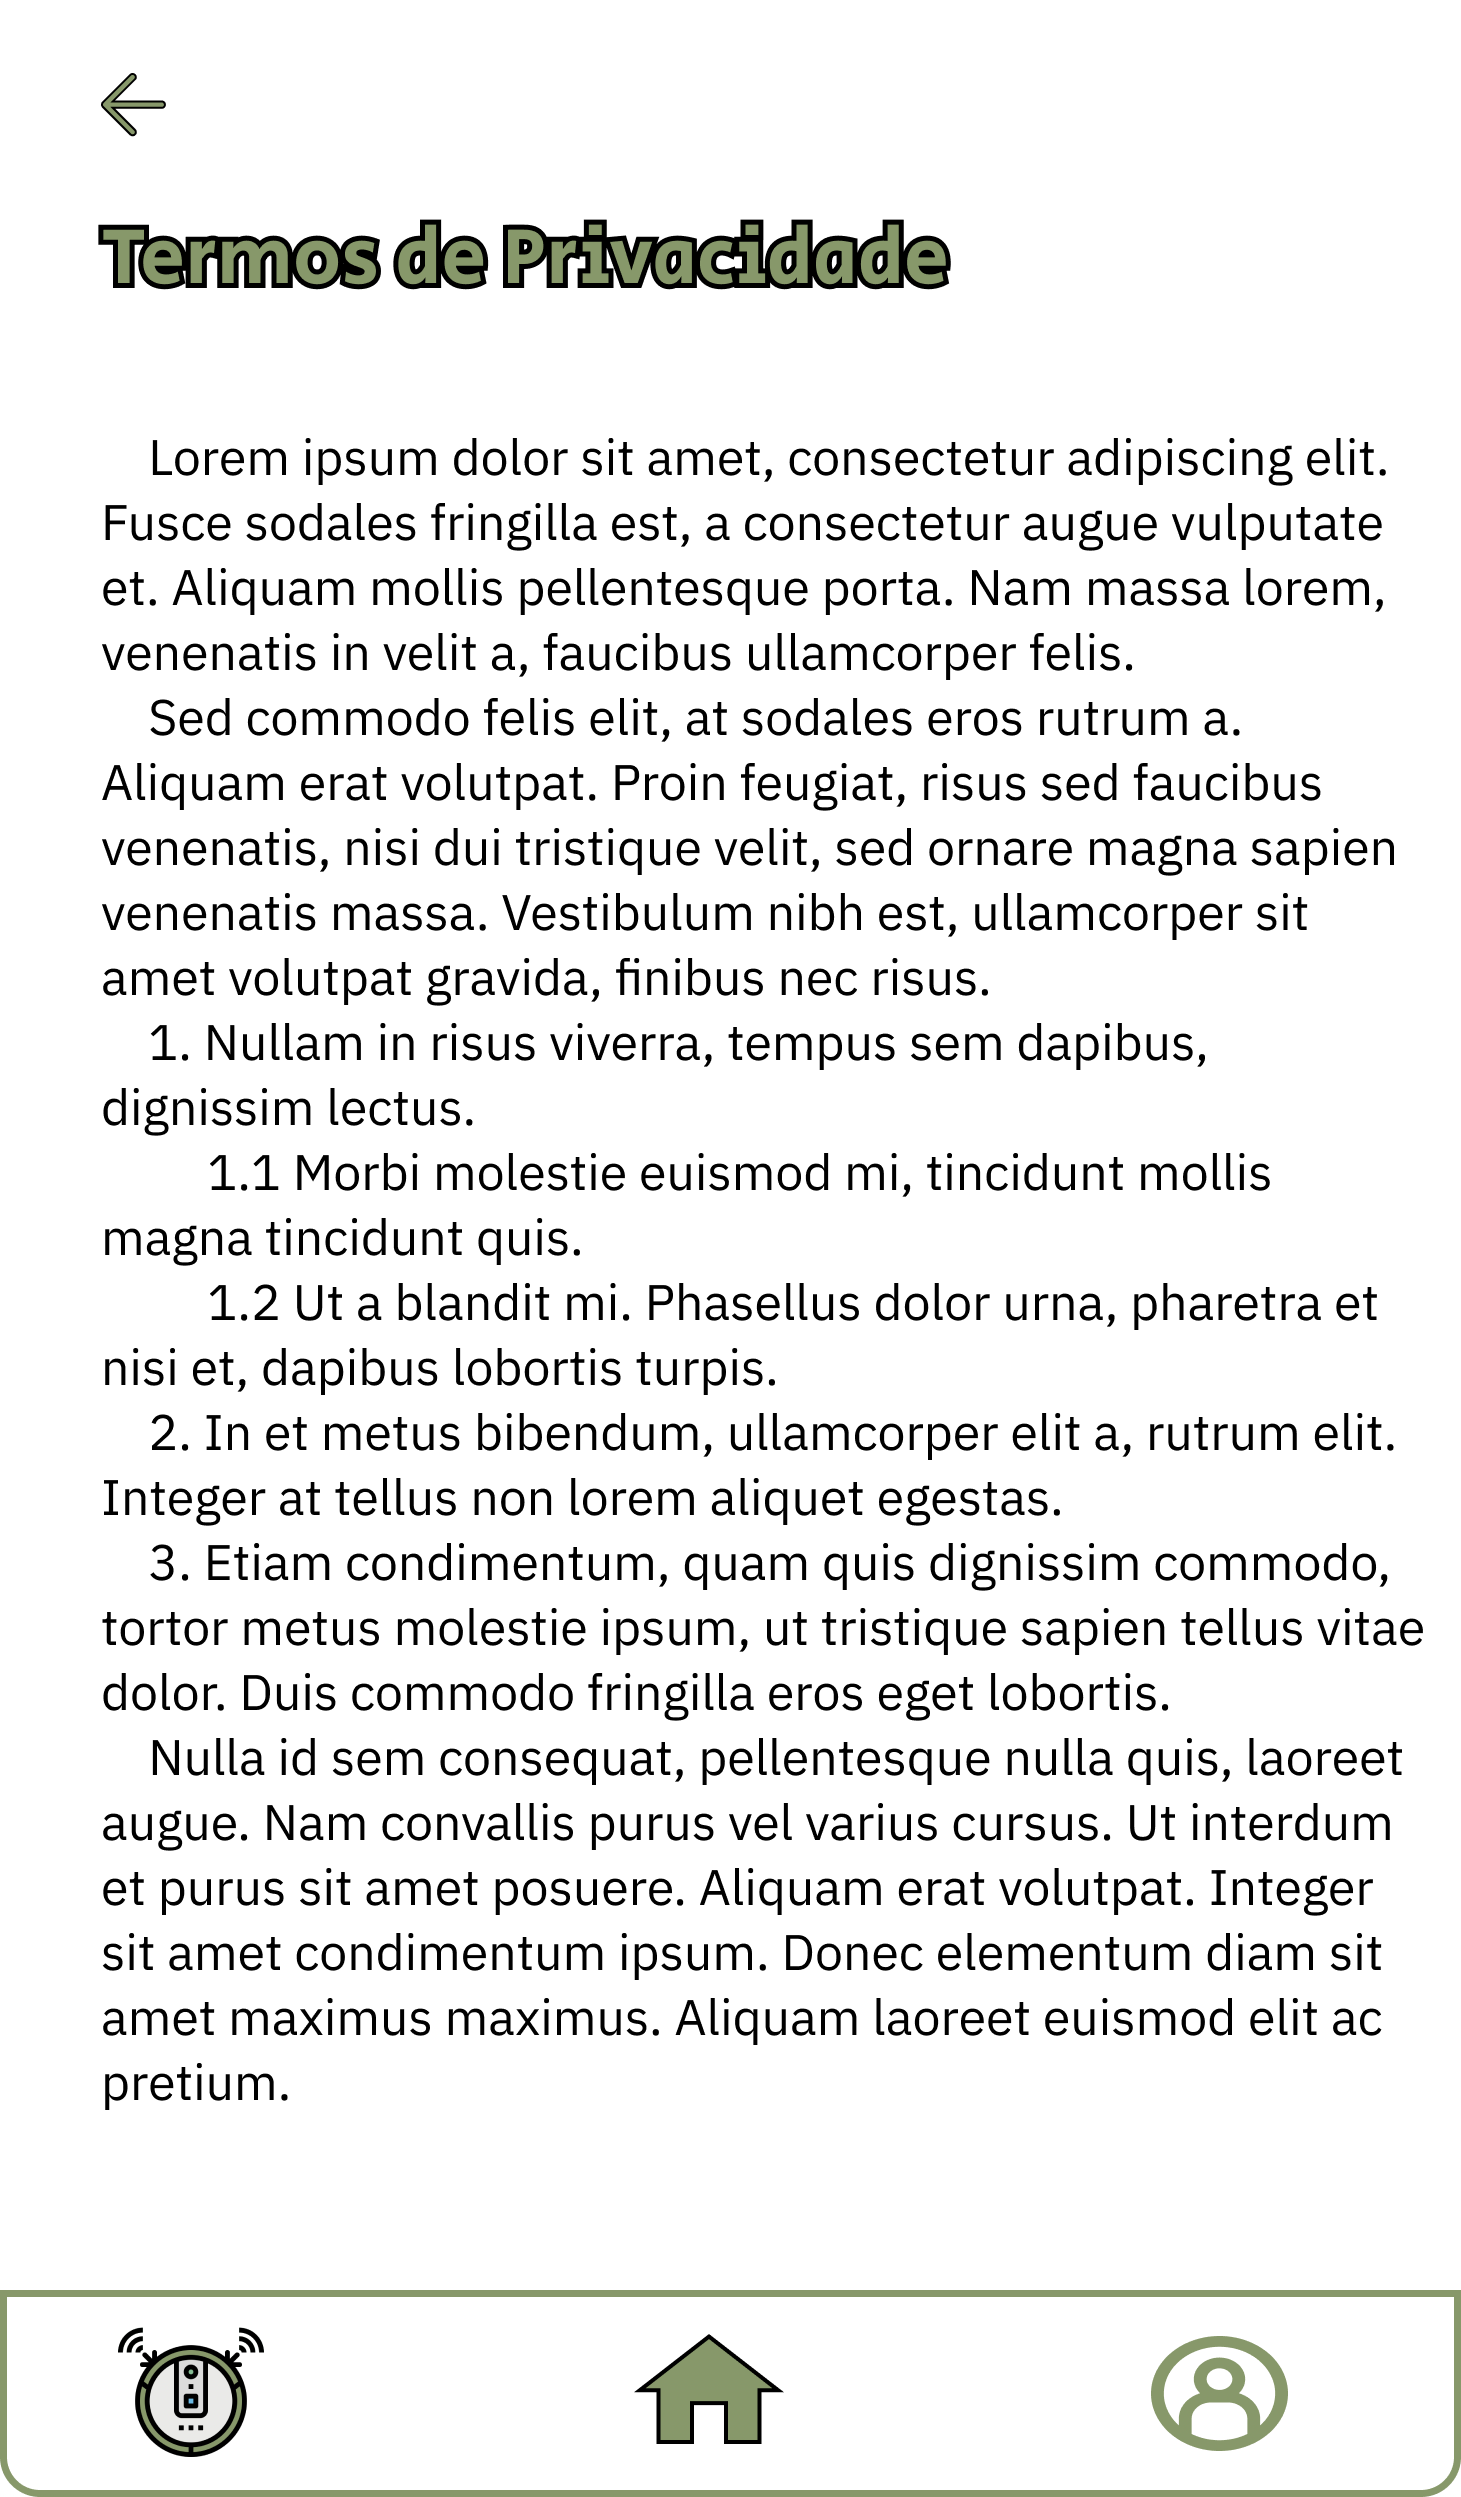
\includegraphics[height=8.5cm]{figuras/Mobile/Privacidade.png}}
\caption{Tela de Termos de Privacidade}
\end{figure}

\subsection{Tela de Modos de Funcionamento}
\begin{figure}[H]
\centering
\frame{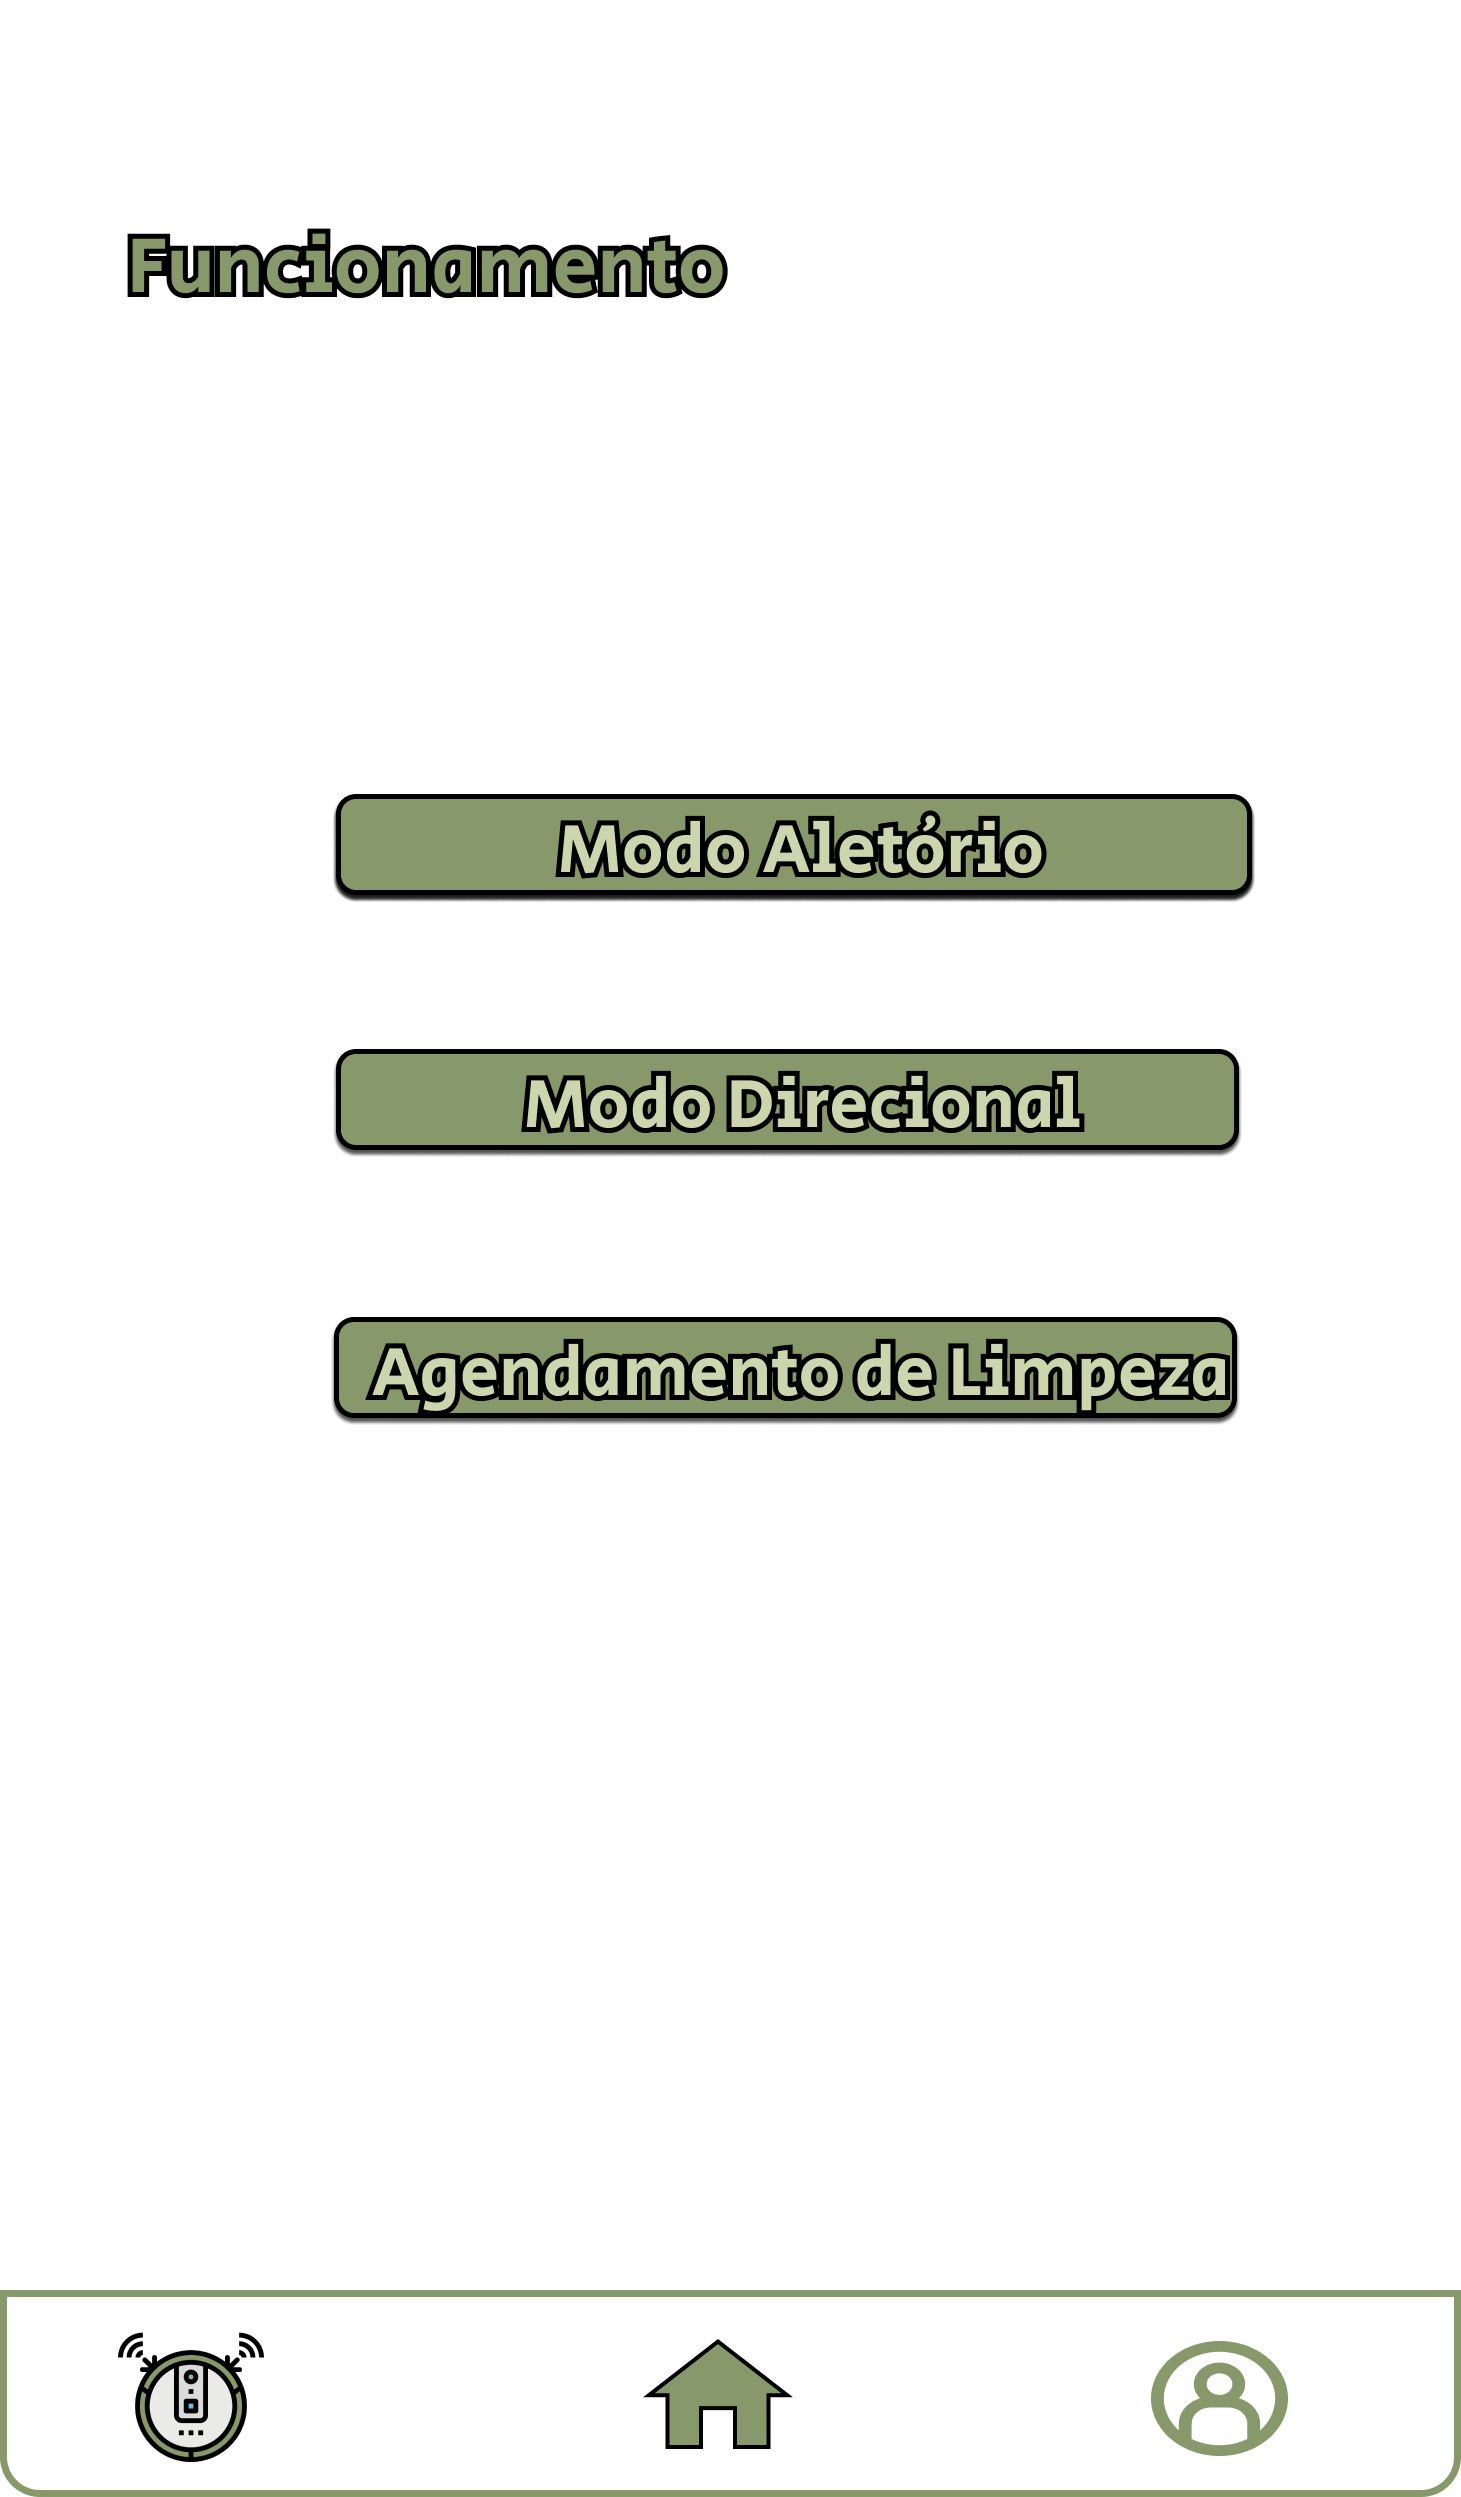
\includegraphics[height=8.5cm]{figuras/Mobile/Funcionamento.png}}
\caption{Tela de  Modos de Funcionamento}
\end{figure}

\subsection{Tela do Modo de Funcionamento Direcional Ativo}
\begin{figure}[H]
\centering
\frame{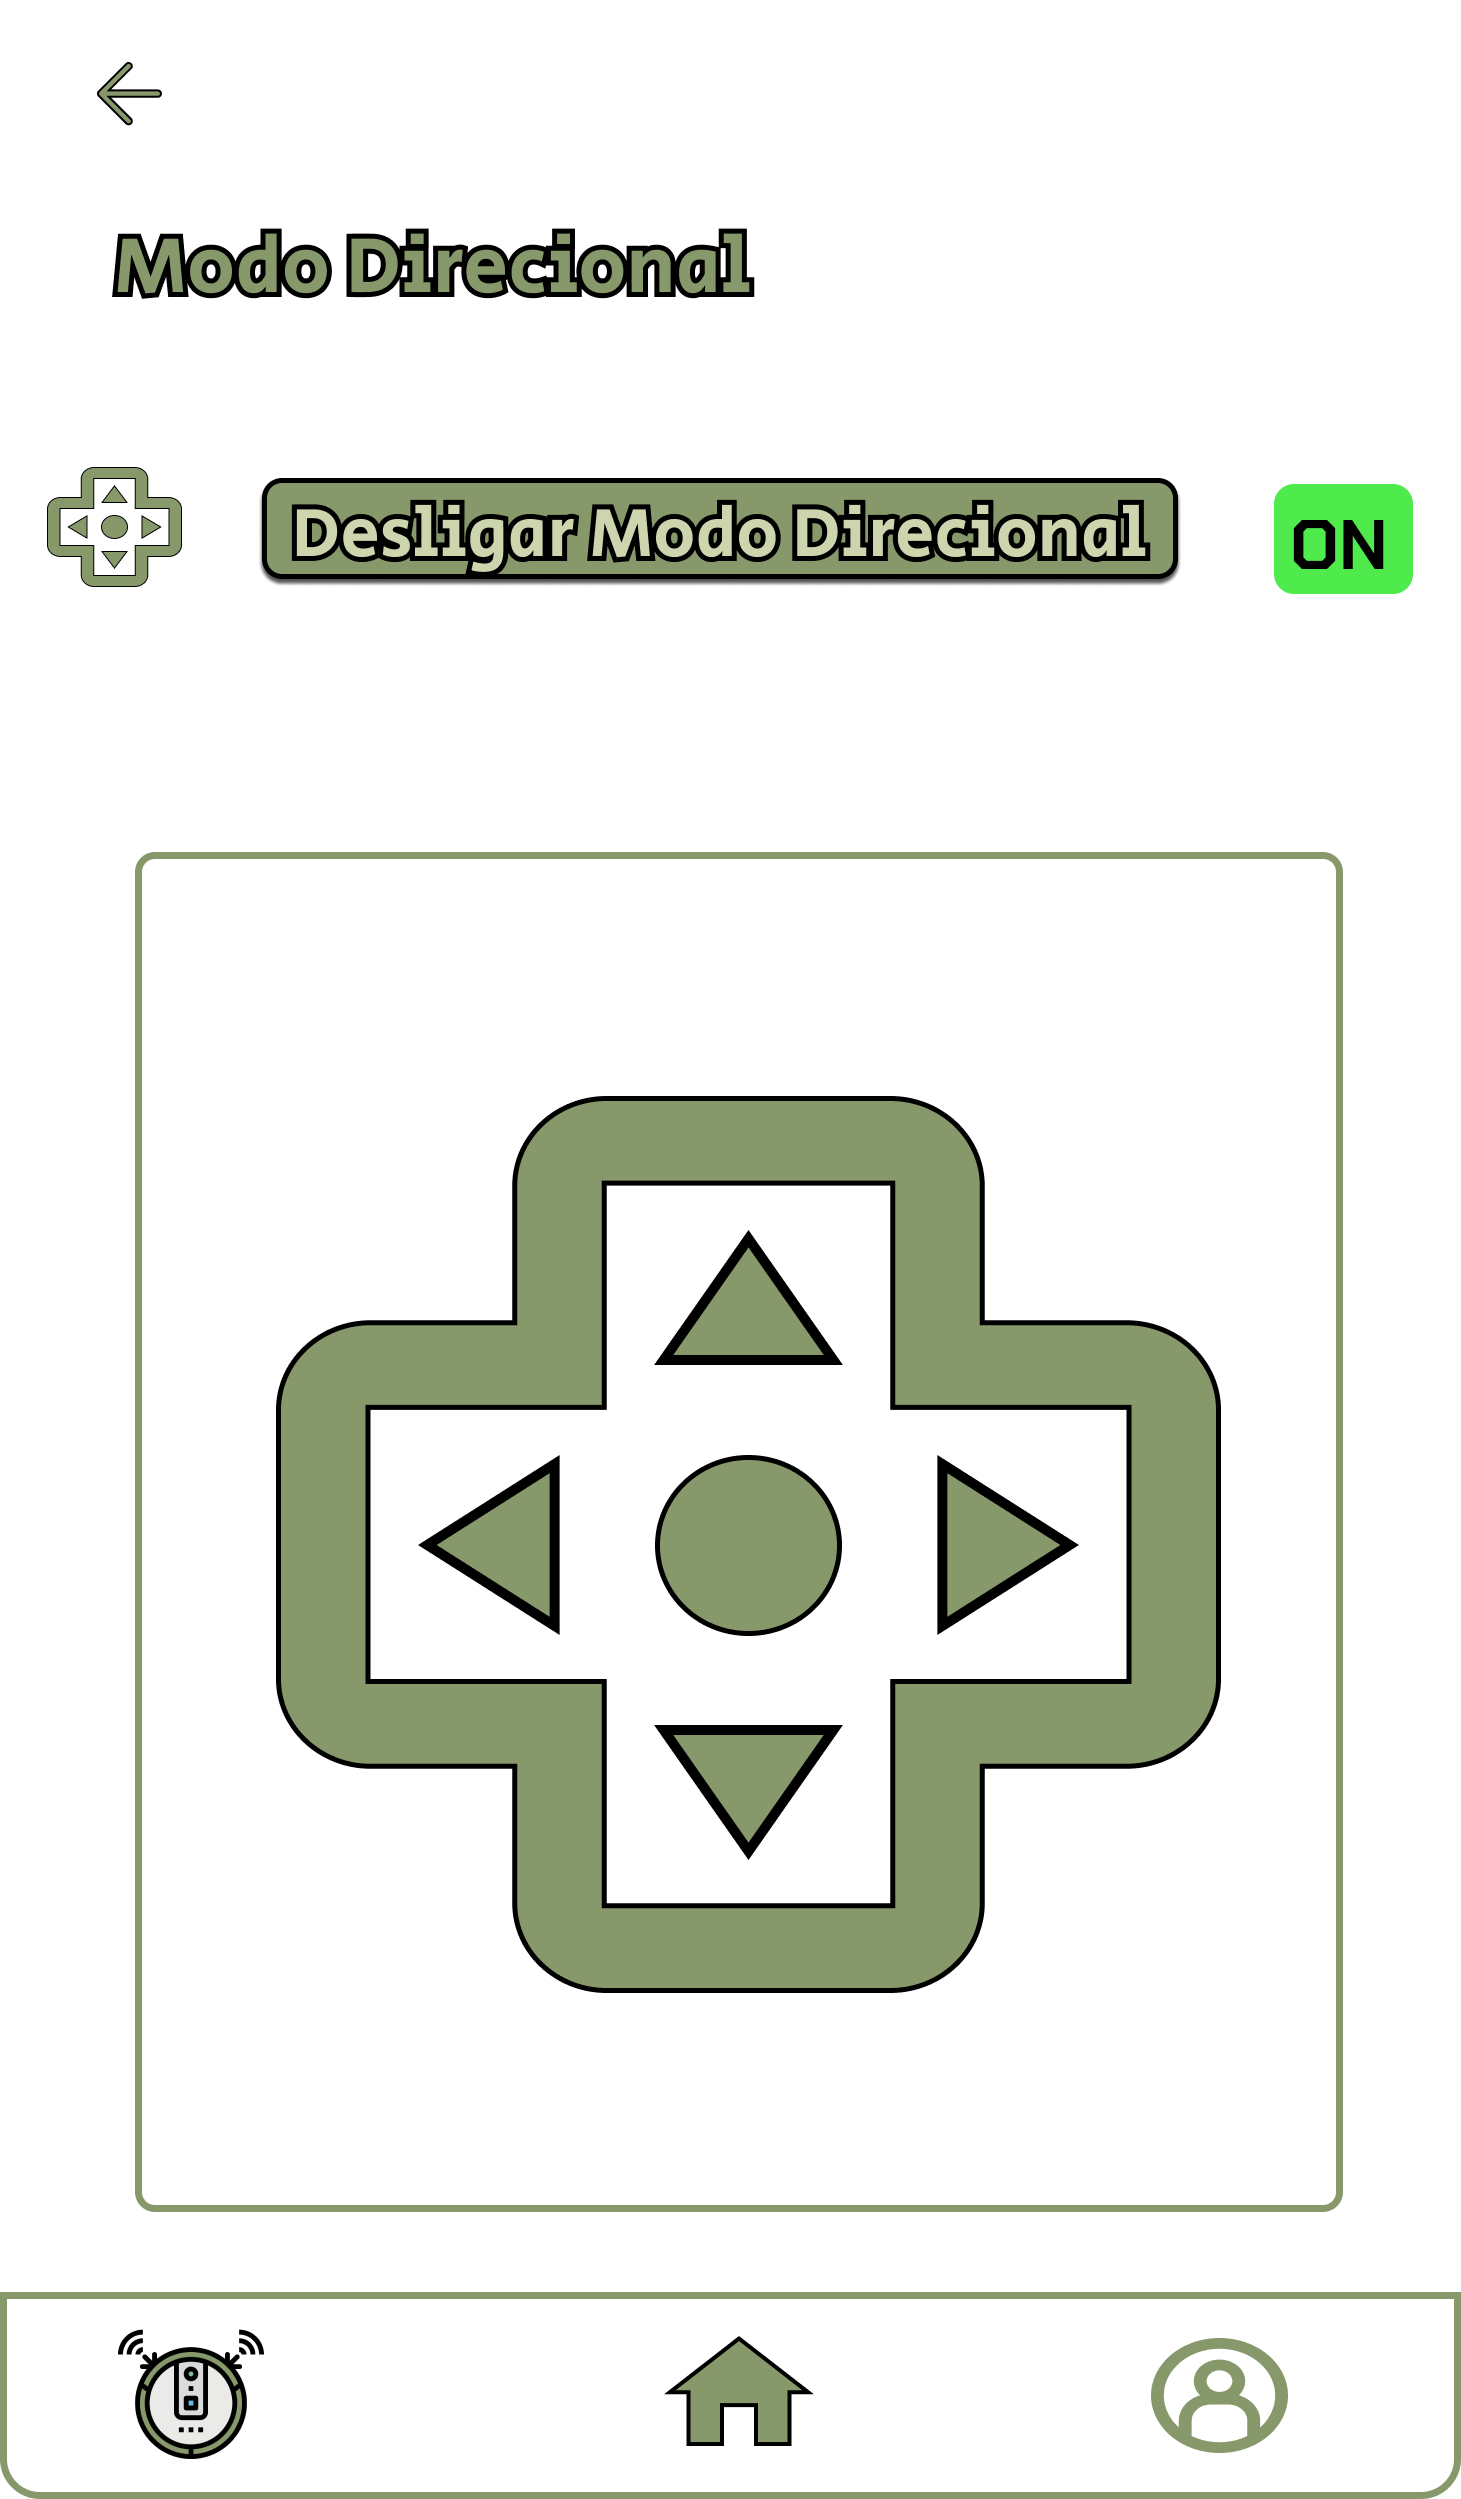
\includegraphics[height=8.5cm]{figuras/Mobile/DirecionalOn.png}}
\caption{Tela do Modo de Funcionamento Direcional Ativo}
\end{figure}

\subsection{Tela do Modo de Funcionamento Direcional Desligado}
\begin{figure}[H]
\centering
\frame{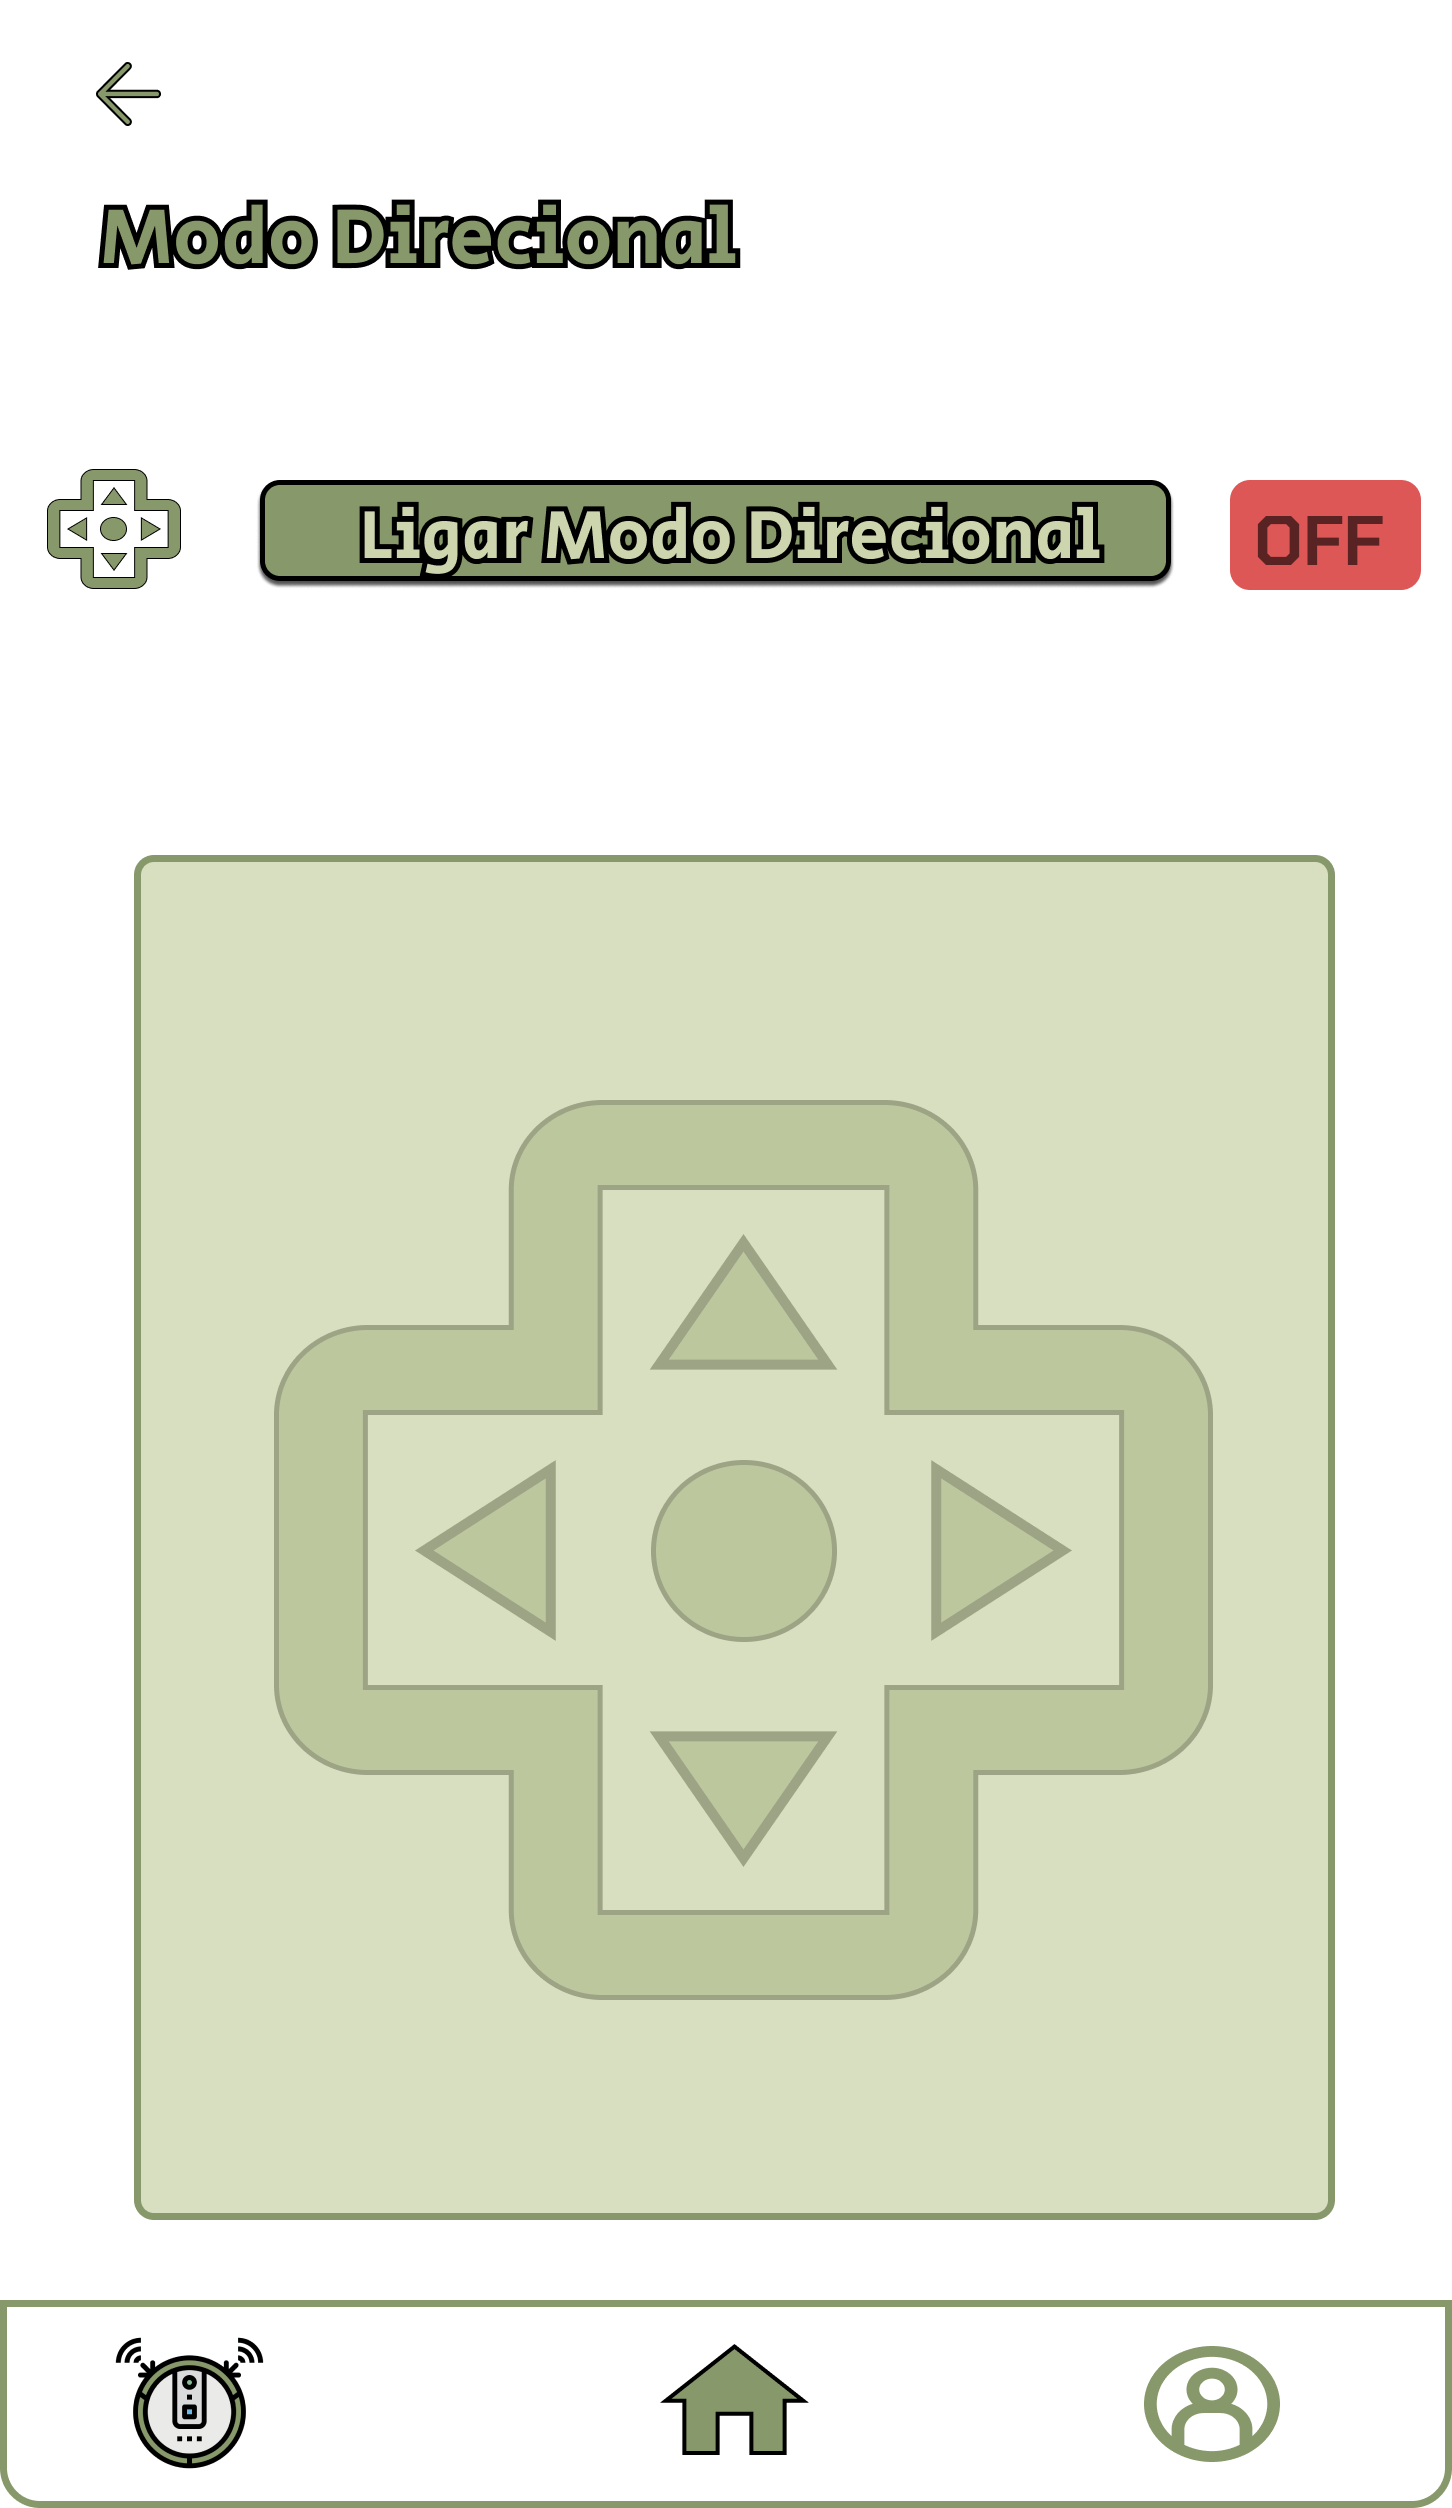
\includegraphics[height=8.5cm]{figuras/Mobile/Mob 14 - Direcional.png}}
\caption{Tela do Modo de Funcionamento Direcional Desligado}
\end{figure}

\subsection{Tela do Modo de Funcionamento Aleatório Ativo}
\begin{figure}[H]
\centering
\frame{\includegraphics[height=8.5cm]{figuras/Mobile/Mob 5 - Aleatório On.png}}
\caption{Tela do Modo de Funcionamento Aleatório Ativo}
\end{figure}

\subsection{Tela do Modo de Funcionamento Aleatório Desligado}
\begin{figure}[H]
\centering
\frame{\includegraphics[height=8.5cm]{figuras/Mobile/Mob 15 - Aleatório.png}}
\caption{Tela do Modo de Funcionamento Aleatório Desligado}
\end{figure}

\subsection{Tela do Agendamento de Limpeza}
\begin{figure}[H]
\centering
\frame{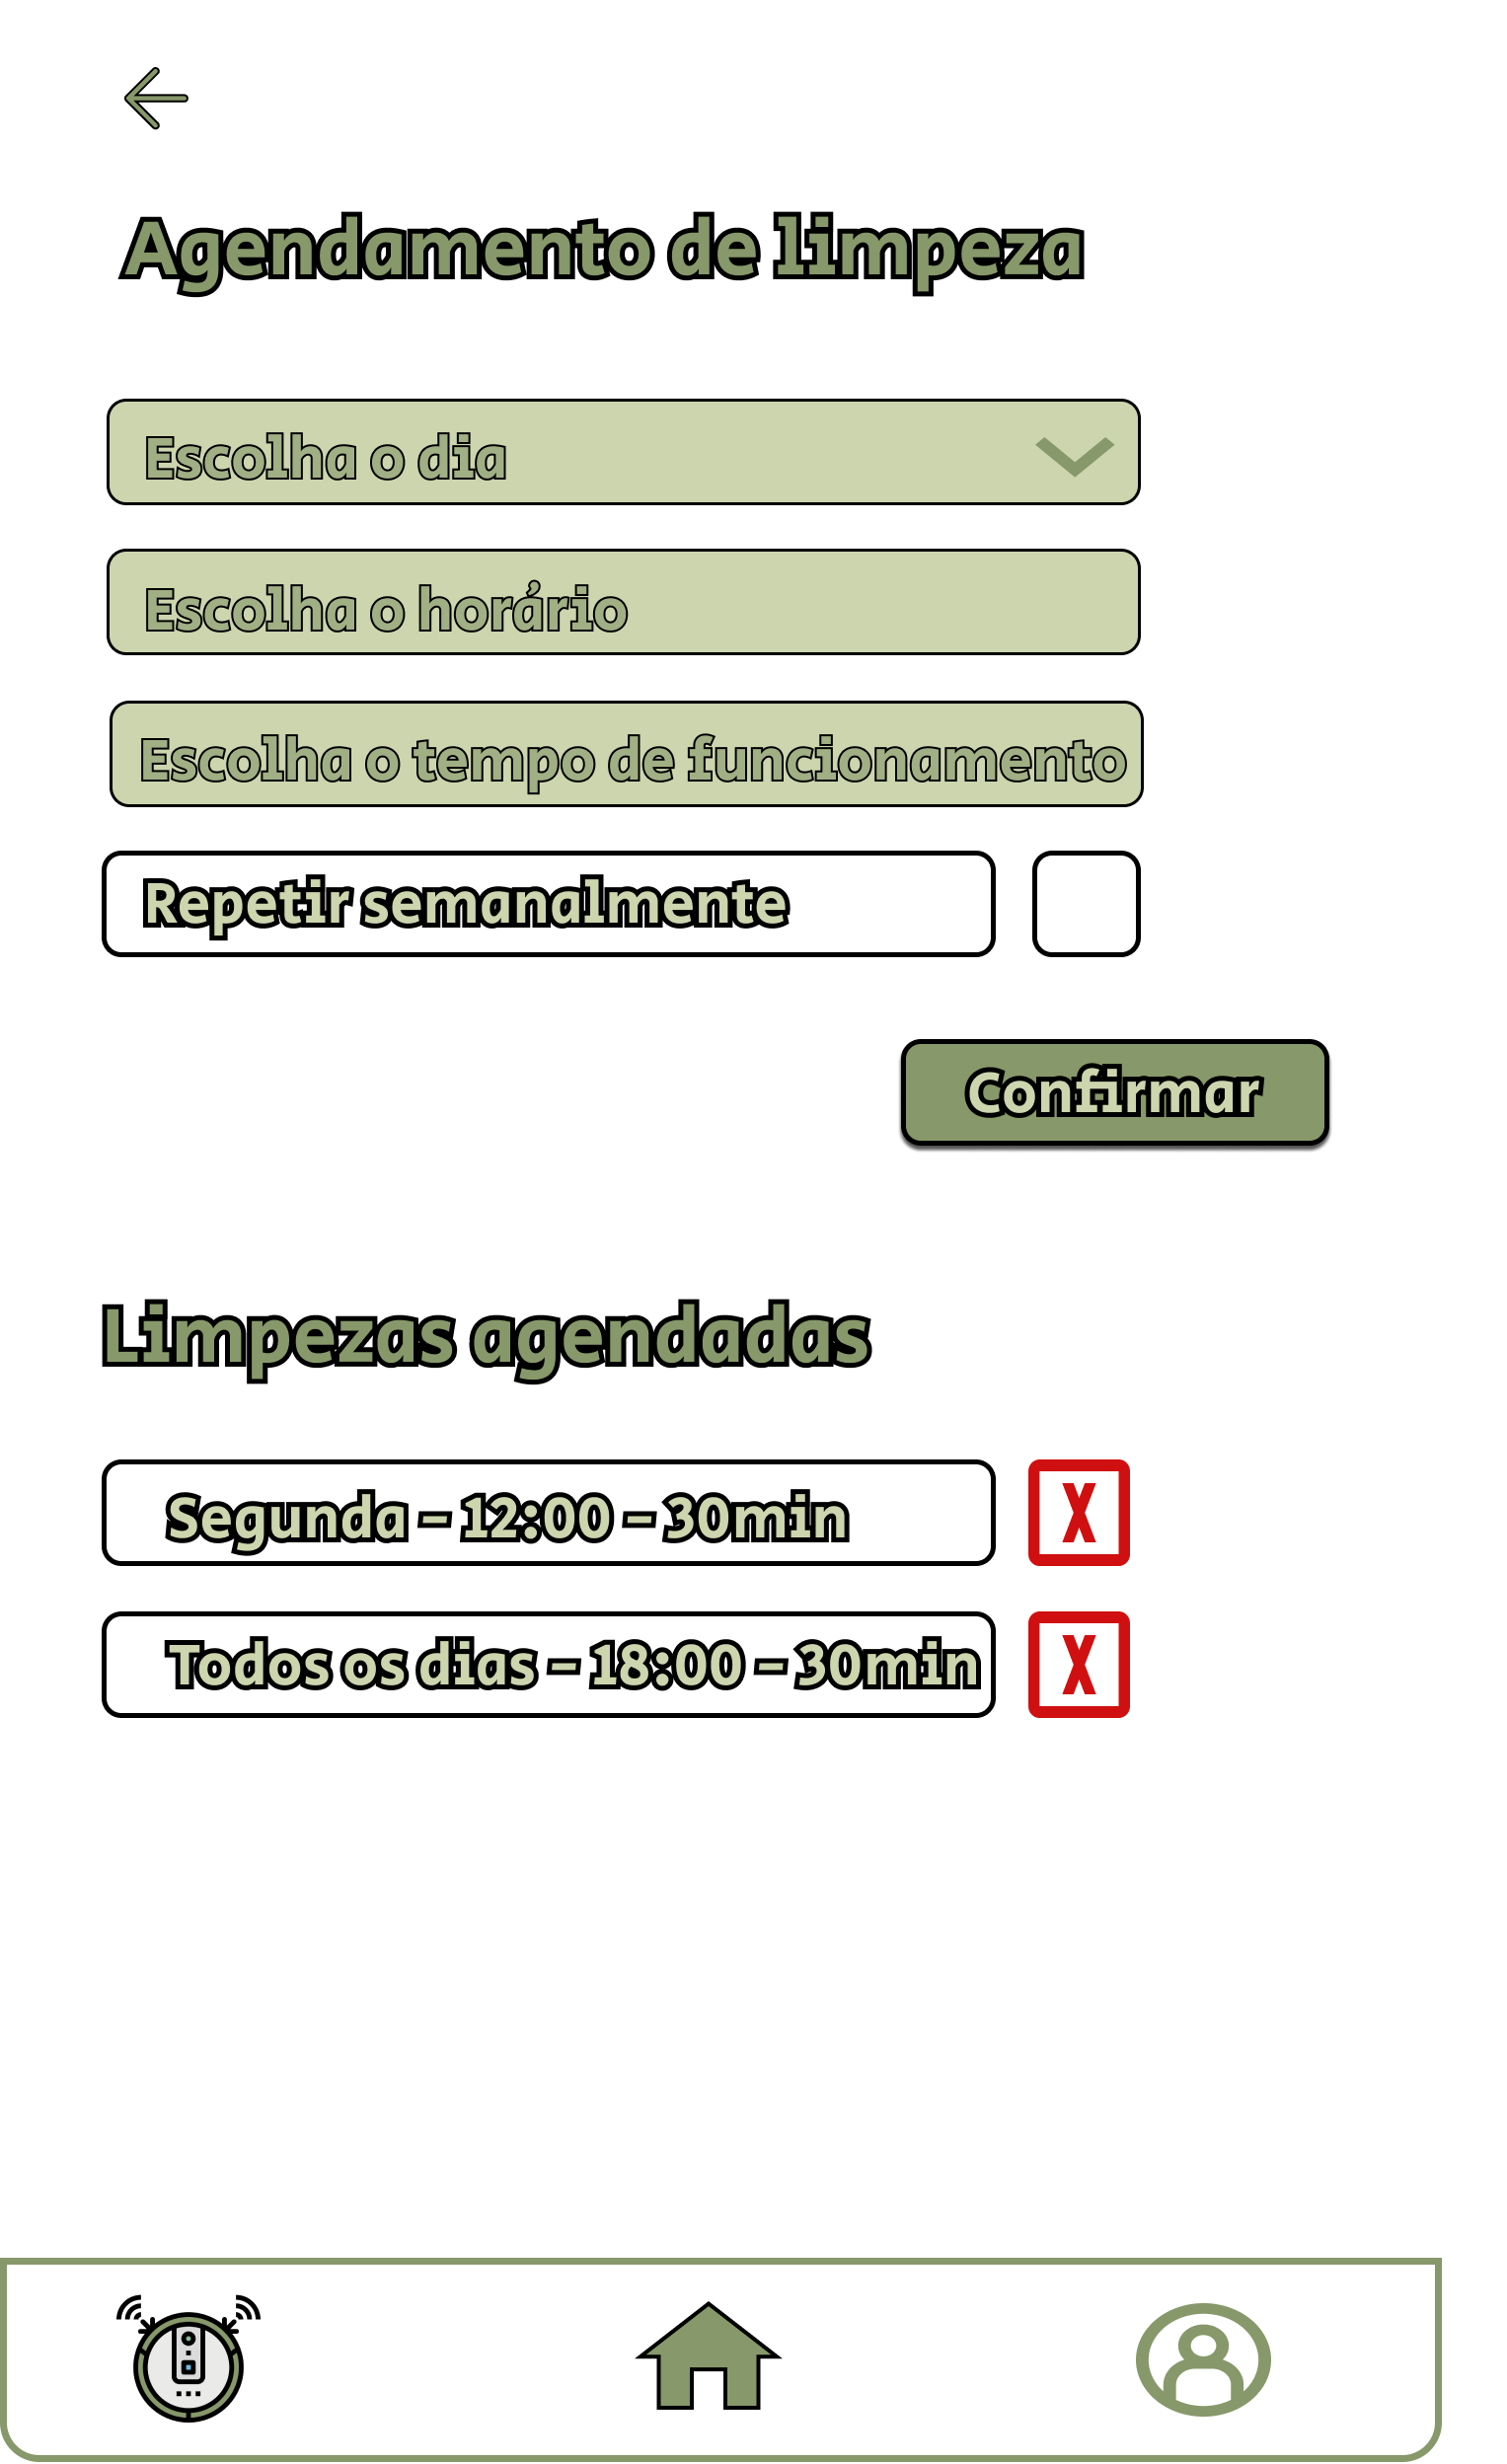
\includegraphics[height=8.5cm]{figuras/Mobile/Mob 13 - Agendamento.png}}
\caption{Tela do Agendamento de Limpeza}
\end{figure}

\section{Diagramas}
\label{diagramaFirmware}
\subsection{Sistema Embarcado}
\subsubsection{Diagrama de Classes}
\label{sec:DiagramaClasses}
\frame{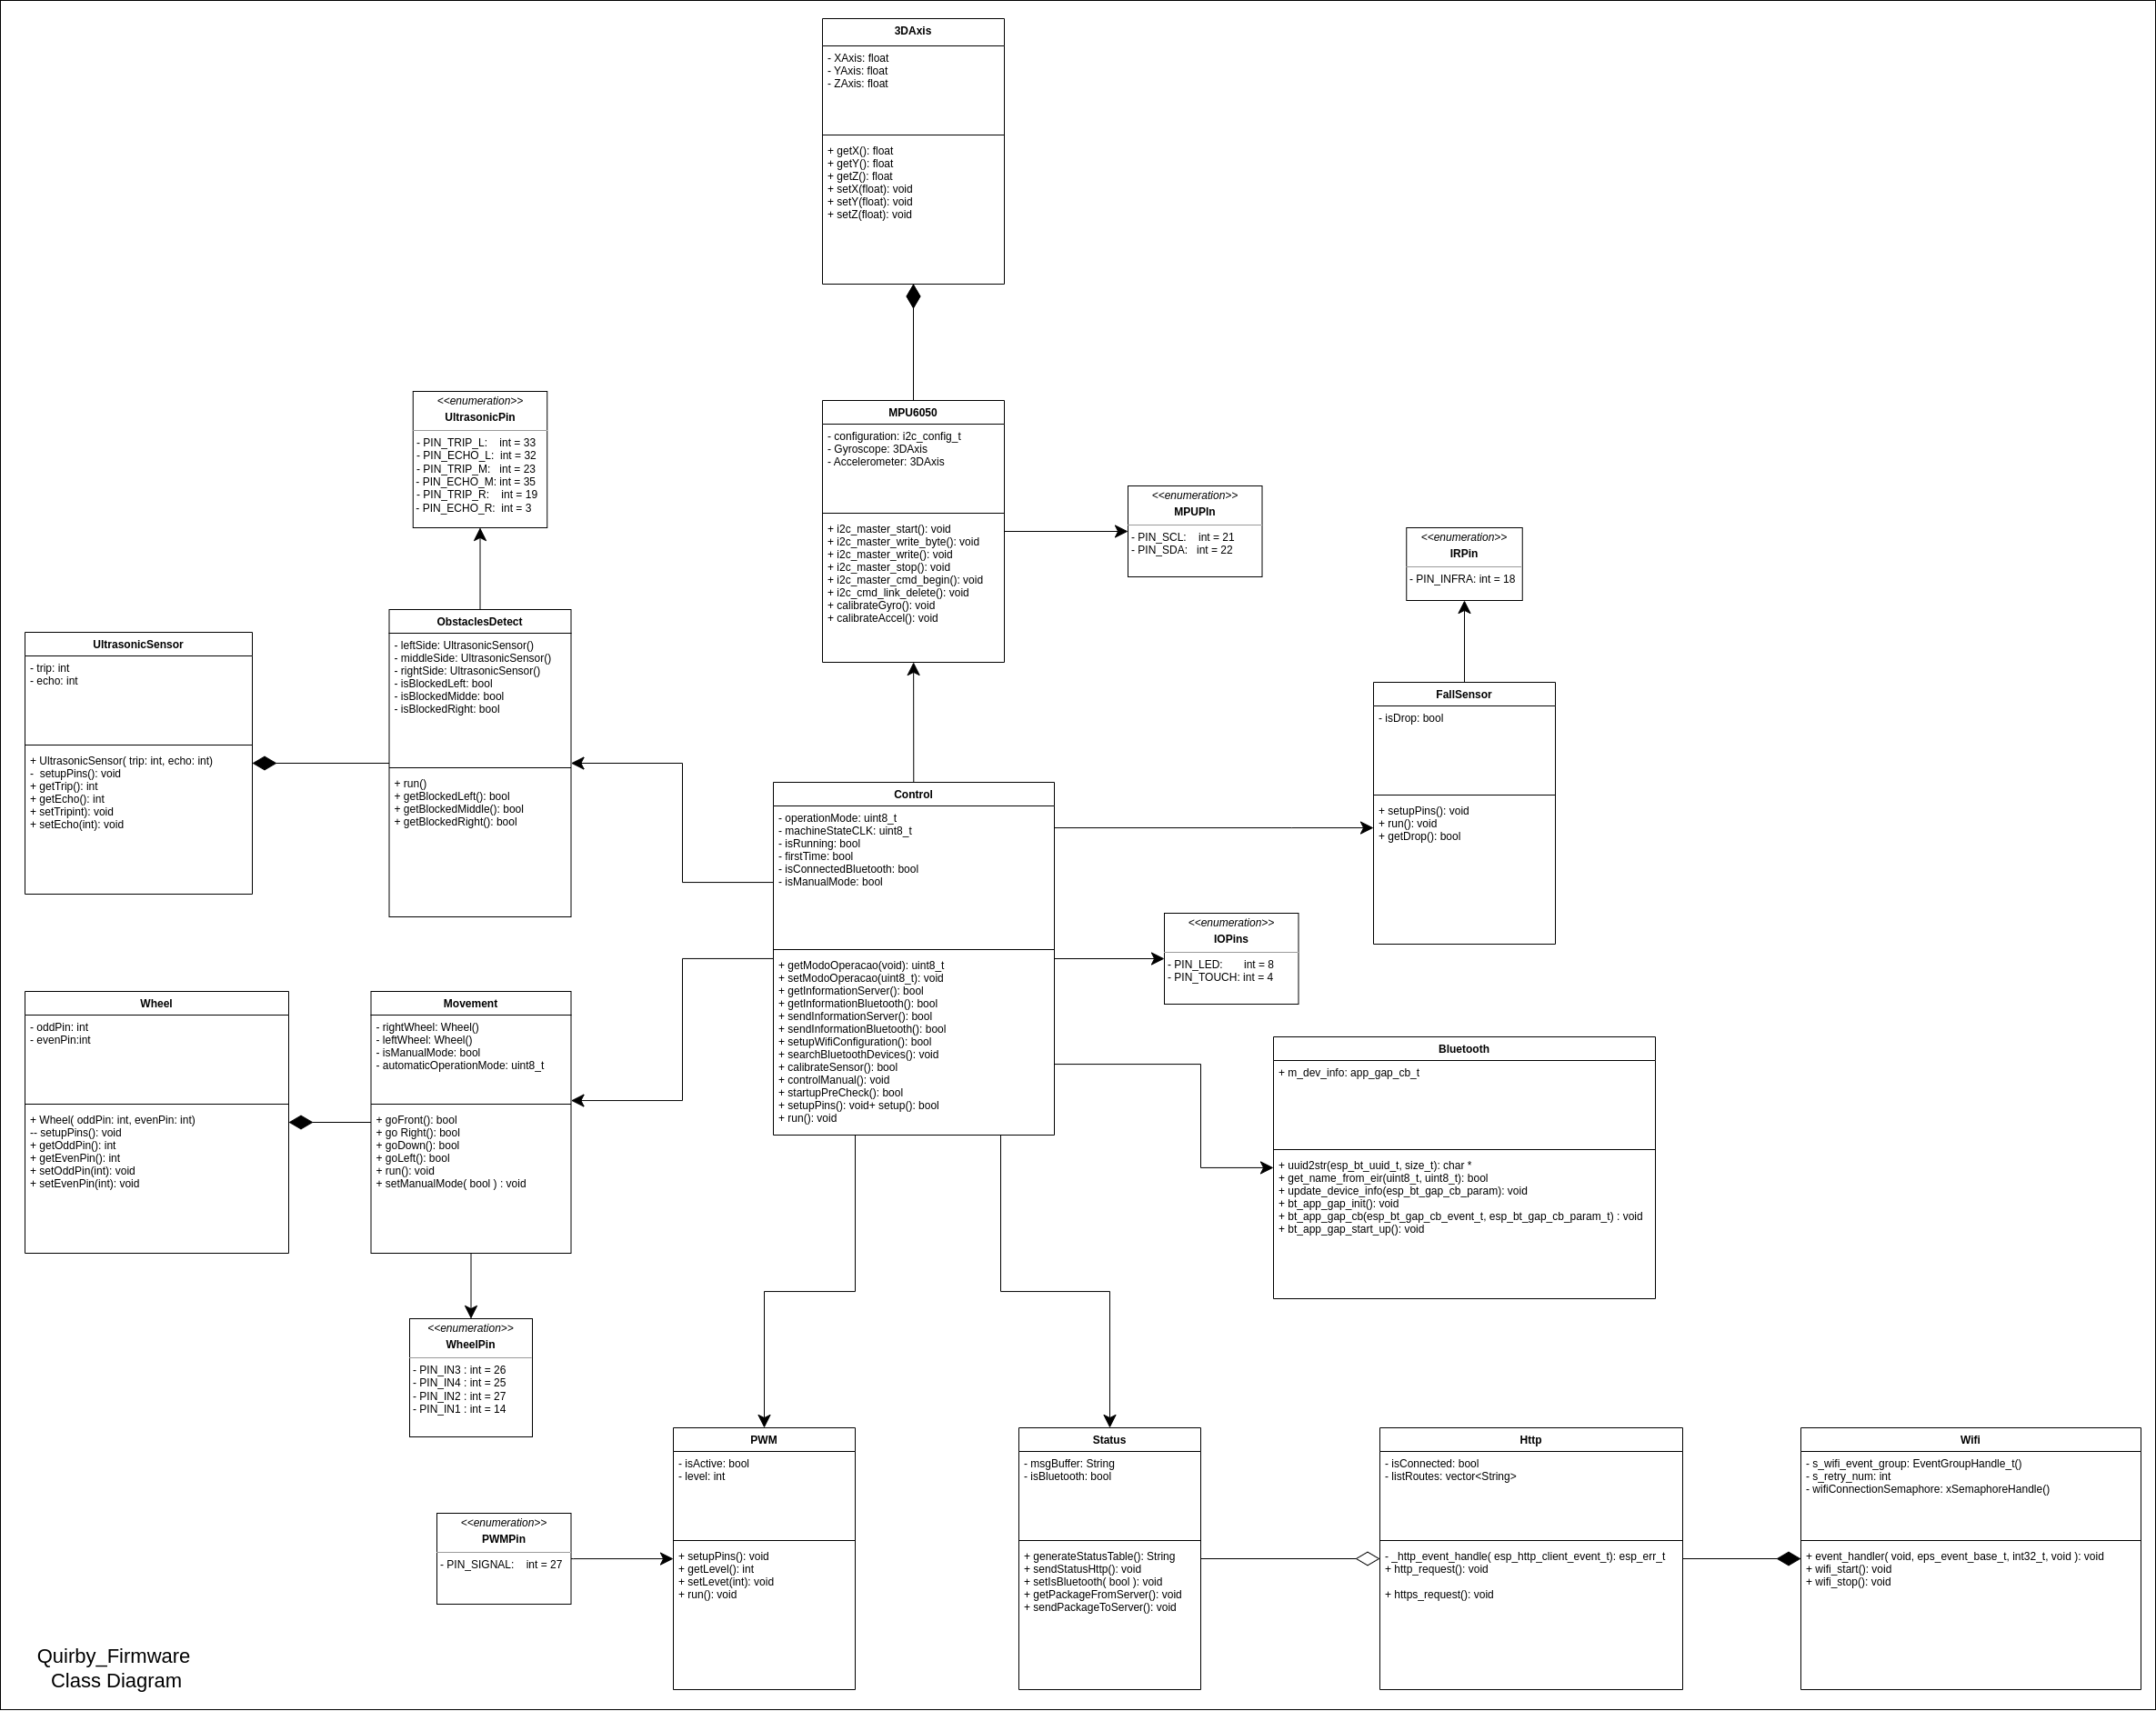
\includegraphics[height=12.0cm]{figuras/software/Diagramas/Embarcados/Quirby_FirmwareDiagramas-Diagrama de Classes.drawio.png}}

\textit{Para melhor visualização, acesse a imagem externamente clicando \href{https://drive.google.com/file/d/1FaDMcYj23tRlHez7_HY8dnomueZytGaC/view?usp=sharing}{aqui}.}

\subsubsection{Diagrama de Sequencia}
\label{sec:DiagramaSequencia}
\frame{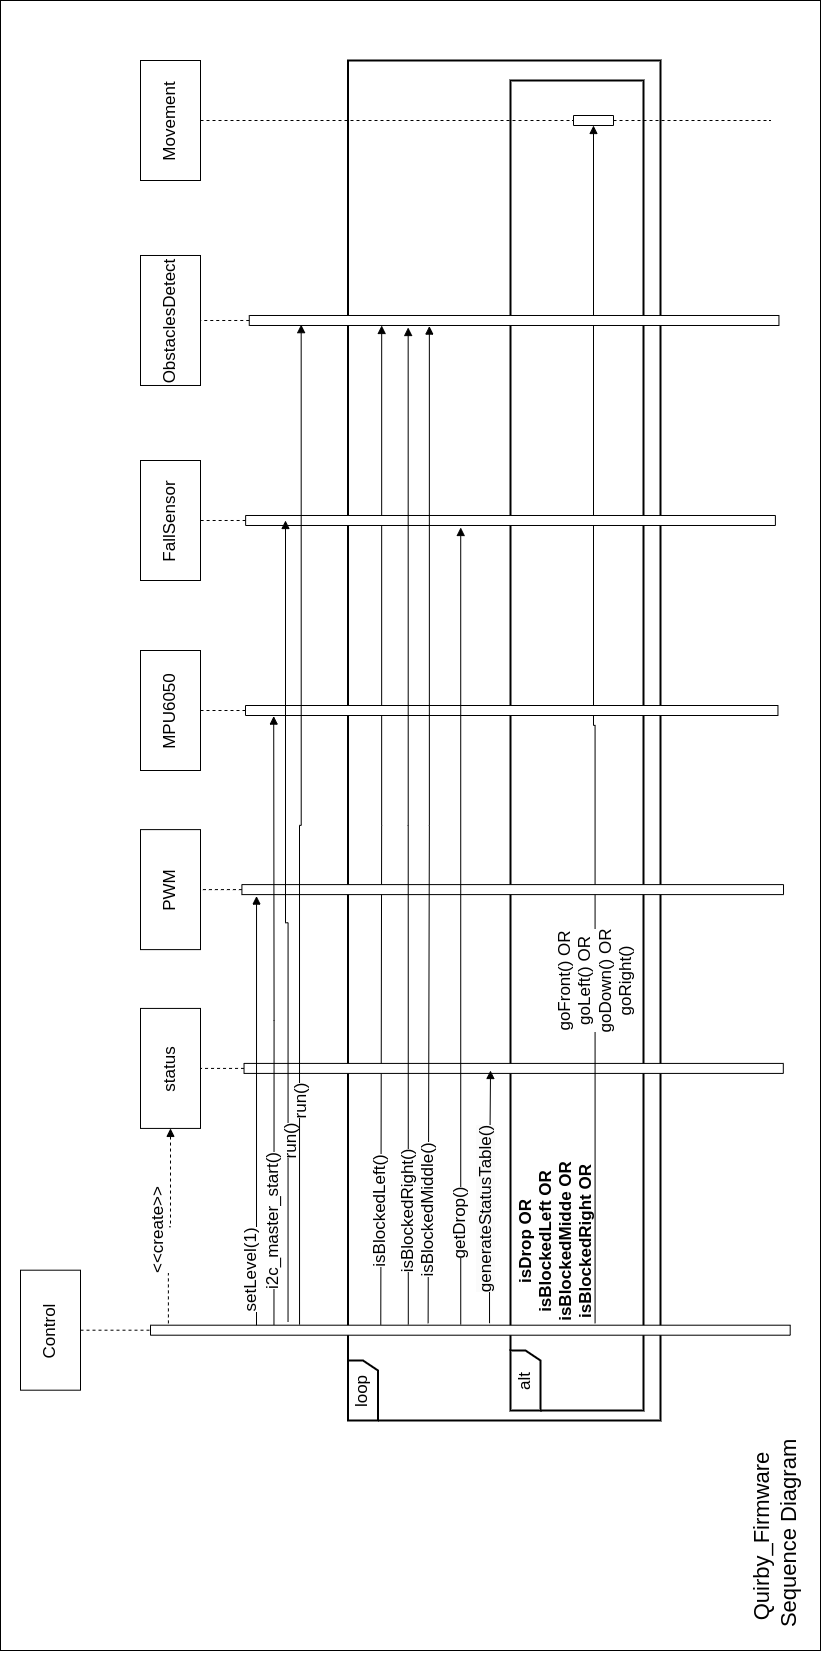
\includegraphics[height=22.0cm]{figuras/software/Diagramas/Embarcados/Quirby_FirmwareDiagramas-Diagrama de Sequência.drawio.png}}

\subsubsection{Diagrama de Pacotes}
\label{sec:DiagramaPacotes}
\frame{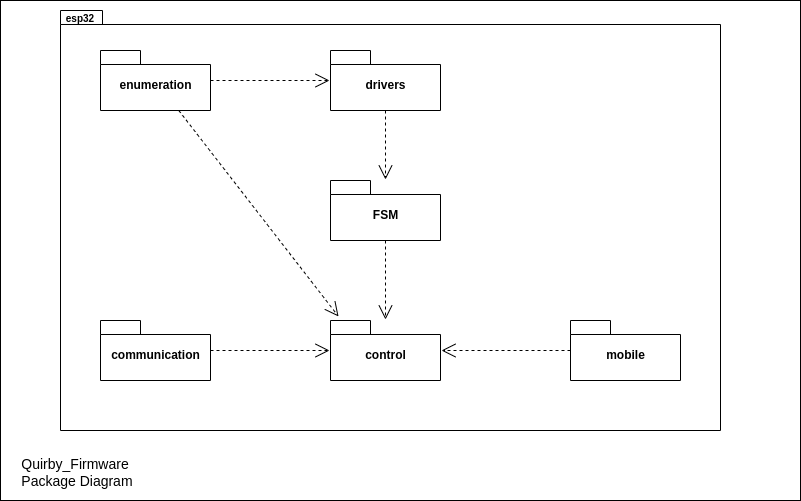
\includegraphics[height=9.0cm]{figuras/software/Diagramas/Embarcados/Quirby_FirmwareDiagramas-Diagrama de Pacotes.drawio.png}}


\chapter{Memorial de cálculo de elementos do projeto}
\section{Autonomia do robô}
O Quirby irá trabalhar em corrente contínua, portanto a energia disponível para sua autonomia será baseada pela quantidade de corrente disponibilizada pela fonte. Desta forma, a equação abaixo demonstra a autonomia teórica do robô.

\begin{equation}
E = Ah = 5000 mAh = 5 Ah
\end{equation}

Sendo E a energia disponível ao sistema. 
A corrente necessária para manter o pleno funcionamento do sistema equivale a cerca de 3,26 A. Portanto, é possível calcular a autonomia teórica em horas do robô.

\begin{equation}
    Autonomia = \frac{5 Ah}{3,26 A}
\end{equation}

\begin{equation}
    Autonomia = 1,53 h = 92 min
\end{equation}

Portanto, desconsiderando as perdas por efeito Joule e por outros fenômenos adversos, a autonomia teórica do robô seria de aproximadamente 92min.

\section{Motor de sucção}
Ao considerar o motor de sucção do projeto como uma máquina de fluxo, é possível utilizar o conceito do balanço de energia para determinar o fluxo mássico do ar.

\begin{equation}
Q-W = m\left(\Delta e+\frac{\Delta P}{\rho}\right)
\end{equation}

Onde:
\begin{itemize}
	\item{Q:} é a quantidade de calor por unidade de tempo que entra na máquina;
	\item{W:} é a quantidade de trabalho por unidade de tempo que a máquina recebe ou fornece ao fluido, neste caso o ar;
	\item{m:} é a quantidade total de massa por unidade de tempo que adentra e sai da máquina. Como não há acumulo de fluido, logo “m” será constante;
	\item{$\Delta$e:} é a variação de todas variações de energia interna do fluido.
	\item {$\Delta$P e \(\rho\):} representam, respectivamente, a variação de pressão causada pelo rotor e a densidade do fluido. Ambos associados representam a energia de pressão do fluido.
\end{itemize}

Dessa forma, podemos simplificar a equação adotando algumas condições, que são:

\begin{itemize}
	\item Não há entrada ou saída de calor da máquina; 
	\item O trabalho será fornecido pela bateria, logo terá valor negativo;
	\item Não há variação significativa da energia interna do fluido.
\end{itemize}

Desse modo, a equação simplifica-se da seguinte forma:

\begin{equation}
W = m\frac{\Delta P}{\rho}
\end{equation}

Ao manipular a equação e isolar o m, temos:

\begin{equation}
m=W\ast\frac{\rho}{\Delta P}
\end{equation}

Adotando os valores obtidos por experimentação, temos:

\begin{itemize}
    \centering
	\item W $=$ 24W;
	\item \(\rho\) $=$ 1,2041 kg/m\textsuperscript{3}
	\item {$\Delta$P} $=$ 1600 Pa.
\end{itemize} \\

\begin{equation}
m=24\ast\frac{1,2041}{1600}
\end{equation}

\begin{equation}
m = 0,018\frac{kg}{s} = 18\frac{g}{s}    
\end{equation}

\vspace{1\baselineskip}
Portanto, o Quirby possui um fluxo teórico de aspiração de partículas por volta de 18 g/s.

\begin{comment}
Este apêndice pode ser utilizado para detalhar as decisões e resultados de testes relacionados ao desenvolvimento de software da solução. 

Deverá ser feito uma subseção para cada elemento de software (Provavelmente não é de software)
\end{comment}

\chapter{Memorial de decisões de desenvolvimento de software}

14/12/2022 -> Decidiu-se usar, para o Backend, a linguagem Javascript com o motor Node.js, com o banco de dados Postgre em conjunto com o Sequelize. Também foi decidido o uso do Docker para o empacotamento. Para o sistema embarcado foi decidido o uso da linguagem de C++ com o framework ESP-IDF. Já para o aplicativo Mobile, optou-se pelo o uso da linguagem Dart com o framework Flutter. Neste mesmo dia foi definida a forma com que cada serviço seria nomeado na \href{https://github.com/orgs/PI2-Grupo5/repositories}{organização} da disciplina. 

22/12/2022 -> Decidiu-se usar a API do Google com o OAuth 2.0 para realizar a autenticação de usuário.

04/01/2022 -> Traçou-se um rascunho para a arquitetura inicial do Firmware, apresentado na Figura \ref{fig:memorial:rascunho_arquitetura}. Este diagrama foi baseado no \href{https://drive.google.com/file/d/1-Vf_cmyCznhIBBIicrbw6bcqnTKv2jFa/view?usp=sharing}{esquemático de eletrônica} elaborado pela equipe do projeto. 

\begin{figure}
    \centering
    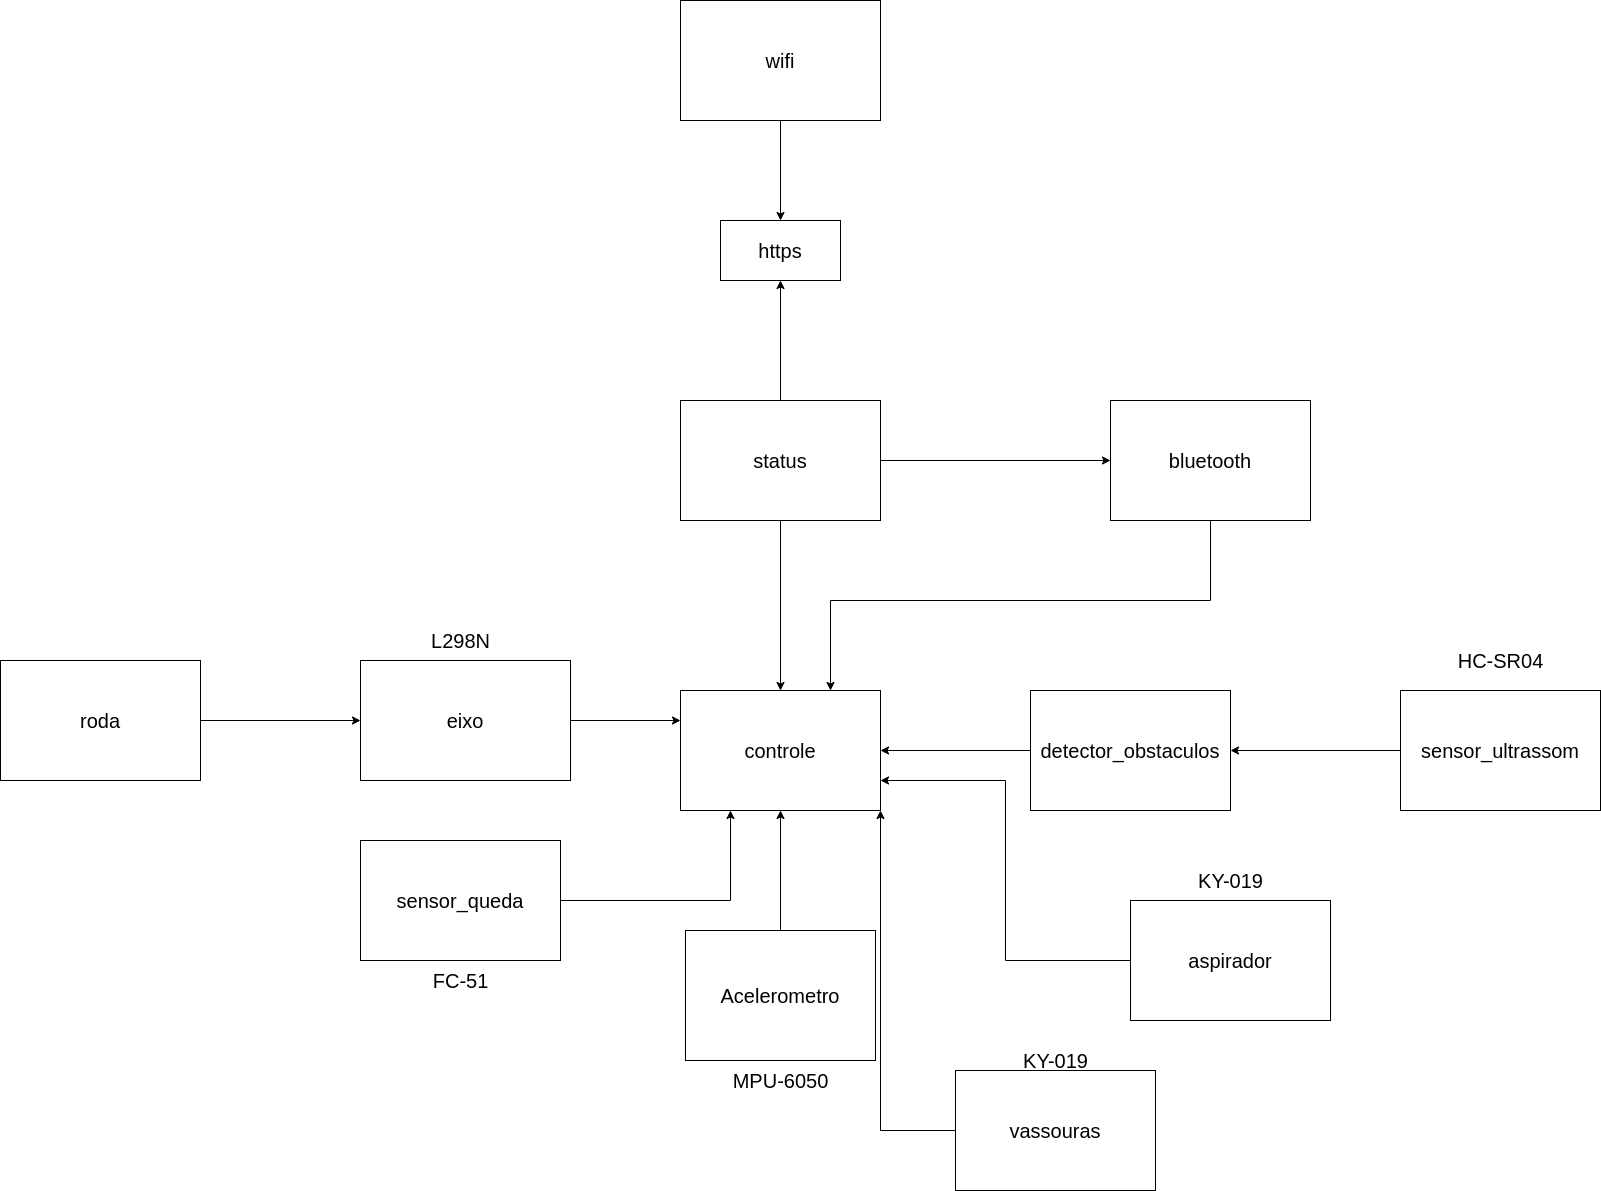
\includegraphics[height=10.5cm]{figuras/software/Memorial/1.png}
    \caption{Rascunho da arquitetura do Quirby Firmware}
    \label{fig:memorial:rascunho_arquitetura}
\end{figure}

06/01/2023 -> Notou-se a necessidade da criação de uma máquina de estados finita no Firmware para o controle da posição e, consequentemente, da movimentação do robô. 

11/01/2023 -> Decidiu-se realizar integração com a assistente virtual Alexa, da Amazon. No tocante ao firmware, optou-se pela criação de uma classe \textit{Movement}, responsável pelo controle do eixo do robô, além dos \textit{enumerations} \textbf{UltrasonicPin} para a classe \textit{ObstaclesDetect}, \textbf{WheelPin} para a classe \textit{Movement}, e \textbf{IRPin} para a classe \textit{FallSensor}. Na modelagem destas classes, definiram-se os relacionamentos de composição entre a \textit{Movement} e a \textit{Wheel}, a \textit{Http} e a \textit{Wifi} e entre a \textit{ObstaclesDetect} e a \textit{UltrasonicSensor} (neste caso, a primeira classe é composta pela segunda).

15/01/2023 -> Optou-se, no contexto do Firmware, utilizar somente uma classe (PWM) para o controle tanto das vassouras, quanto do motor de aspiração, e da utilização de somente uma classe (MPU6050) para o controle do Giroscópio e do Acelerômetro, sendo esta composta pela classe \textit{3DAxis}, responsável pelo controle da posição do robô no espaço. Foram acrescidos também os \textit{enumerations} \textbf{IOPins} à classe \textit{Control}, \textbf{MPUPin} à classe \textit{MPU6050} e \textbf{PWMPin} à classe \textit{PWM}. Estas mudanças resultaram no \hyperref[sec:DiagramaClasses]{Diagrama de Classes} final do Firmware do Quirby. Tendo então esta arquitetura definida, foram desenvolvidos o \hyperref[sec:DiagramaSequencia]{Diagrama de Sequência} e \hyperref[sec:DiagramaPacotes]{de Pacotes} para o Firmware.

\chapter{Autoavaliação dos Integrantes}
\centering
\begin{table}[H]
\caption{\label{tab 15} Autoavaliação dos Integrantes}

\begin{tabular}{ |>{\centering\arraybackslash} m{5cm}|>{\centering\arraybackslash} m{11.5cm} |}


\hline
\rowcolor[HTML]{D9D9D9} 
\multicolumn{1}{|c|}{\cellcolor[HTML]{D9D9D9}\textbf{INTEGRANTE}} & \multicolumn{1}{c|}{\cellcolor[HTML]{D9D9D9}\textbf{CONTRIBUIÇÃO}}                                                                                                                                                                                                                                                                                  \\ \hline
\rowcolor[HTML]{DBEEF3} 
Alander Praxedes de Souza Oliveira                                & \begin{tabular}[l]{@{}l@{}}Participação da Lean Inception; Participação das reuniões de \\ eletrônica e detalhamento dos principais componentes; Gerência\\ das atividades iniciais no escopo da eletrônica.\end{tabular}                                                                                                                     \\ \hline
\rowcolor[HTML]{DBEEF3} 
Bruno Carmo Nunes                                                 & \begin{tabular}[l]{@{}l@{}}Participação da Lean Inception, e das discussões do escopo do \\ projeto; Criação da documentação de riscos e custos do projeto; \\ Auxiliou na criação do EAP, nos requisitos funcionais, e \\ também na arquitetura de software. Também teve participação \\ na formatação do relatório.\end{tabular} \\ \hline
\rowcolor[HTML]{DBEEF3} 
Estéfane Mendes do Nascimento                                     & \begin{tabular}[c]{@{}l@{}}Participação da Lean Inception; Termo de Abertura do Projeto,\\ participação em todas as discussões do grupo. Conversão do \\ documento para LaTex. Teste do motor. Vídeo de \\ propaganda. Revisão do relatório. \end{tabular}                                                                                                      \\ \hline
\rowcolor[HTML]{DBEEF3} 
Estevão de Jesus Reis                                             & \begin{tabular}[c]{@{}l@{}}Participação da Lean Inception e de todas as discussões do \\ escopo do projeto, descreveu o cronograma de atividades,  \\ auxiliou na organização das reuniões.\end{tabular}                                                                                                                                          \\ \hline
\rowcolor[HTML]{DBEEF3} 
Fernando Souza Braga                                              & \begin{tabular}[c]{@{}l@{}}Participação da Lean Inception. Participou das \\ reuniões de eletrônica e detalhamento dos \\ principais componentes e auxiliou o \\ desenvolvimento de textos.\end{tabular}                                                                                                                                            \\ \hline
\rowcolor[HTML]{DBEEF3} 
Gabriel Azevedo Batalha                                           & \begin{tabular}[c]{@{}l@{}}Participação da Lean Inception e de discussões \\ de escopo do projeto. Elaboração da EAP e do \\ plano de comunicação. Auxílio em outros tópicos \\ no apêndice A e E, organização de reuniões e revisão \\ do relatório em geral. Participação na concepção dos \\ diagramas do Backend\end{tabular}                                                                                      \\ \hline
\rowcolor[HTML]{DBEEF3} 
Giovana Vitor Dionisio Santana                                    & \begin{tabular}[c]{@{}l@{}}Participação da Lean Inception; Participação nas discussões do \\ escopo do projeto e auxílio na apresentação dos requisitos; \\ Definição/desenvolvimento da arquitetura de software; Revisão\\ e formatação do relatório.\end{tabular}                                                                                                          \\ \hline
\rowcolor[HTML]{DBEEF3} 
Gustavo Raspante Faria                                            & \begin{tabular}[c]{@{}l@{}}Participação da Lean Inception. Participação nas reuniões\\ de eletrônica e detalhamento dos principais componentes \\ e auxiliou o desenvolvimento de textos.\end{tabular}                                                                                                                                              \\ \hline
\rowcolor[HTML]{DBEEF3} 
Hérya Rodrigues Alcantara                                         & \begin{tabular}[c]{@{}l@{}}Participação da Lean Inception e de discussões do escopo \\ do projeto; Elaboração da EAP; Explanação da Metodologia \\ dos Objetivos específicos do projeto; auxiliou em tópicos dos \\ Apêndices A e D; organização de reuniões e divisão de tarefas; \\ correção, revisão e formatação do relatório; elaboração do \\ protótipo; participação no projeto do frontend de software. \end{tabular}                                                                                                                    \\ \hline
\end{tabular}
\end{table}
\begin{table}[H]
\begin{tabular}{ |>{\centering\arraybackslash} m{5cm}|>{\centering\arraybackslash} m{11.5cm} |}
\hline
\rowcolor[HTML]{D9D9D9}
\rowcolor[HTML]{DBEEF3} 
\rowcolor[HTML]{DBEEF3} 
João Paulo Coelho de Souza                                        & \begin{tabular}[c]{@{}l@{}}Participação da Lean Inception, participação em todas as \\ reuniões de discussão do escopo do projeto, auxílio na \\ criação dos documentos de requisitos e arquitetura de \\ software, correção e revisão relatório. elaboração do protótipo; \\ participação no projeto do frontend de software com criação de \\ telas e integração com o back-end da aplicação.
\end{tabular}
           \\ \hline
           \rowcolor[HTML]{DBEEF3} 
Marcos Vinícius Rodrigues da Conceição                            & \begin{tabular}[c]{@{}l@{}}Participação da Lean Inception, e das discussões do \\ escopo do projeto, realizou a criação da documentação \\ de riscos e custos do projeto, formatação e revisão do \\ relatório, descrição dos gastos energéticos do sistema, \\ revisão do relatório e organização das reuniões, criação da\\ documentação de arquitetura, criação de diagramas conceituais,\\ lógico e código SQL da aplicação.\end{tabular}                       \\ \hline
\rowcolor[HTML]{DBEEF3} 
Matheus Rodrigues de C. Silva                                     & \begin{tabular}[c]{@{}l@{}}Participação das reuniões de estruturas, confecção dos CADs \\e desenhos técnicos, detalhamento dos componentes, material e \\desenvolvimento do texto.\end{tabular}                                                                                                                                                                                              \\ \hline
\rowcolor[HTML]{DBEEF3} 
Murilo de Souza Barcelos                                          & \begin{tabular}[c]{@{}l@{}}Participação da Lean Inception, formatação e revisão \\do relatório, desenvolvimento dos \\resultados nos cálculos de fluxo e gasto energético.\end{tabular}                                                                                                                                                                                                        \\ \hline
\rowcolor[HTML]{DBEEF3} 
Igo de frança lino                                                & \begin{tabular}[c]{@{}l@{}}Participação das reuniões de estruturas, detalhamento \\ dos componentes, material e desenvolvimento do texto.\end{tabular}                                                                                                                                                                                              \\ \hline

\end{tabular}
\end{table}